\documentclass[10pt]{article}
\usepackage[margin=2.2cm]{geometry}
\usepackage{booktabs,longtable,graphicx,array}
\usepackage[hidelinks]{hyperref}
\setlength{\tabcolsep}{4pt}
\newcommand{\stackcell}[1]{\begin{tabular}[t]{@{}l@{}}#1\end{tabular}}
\title{tropical: ConvexHull}
\date{2026-10-26T03:17:59}
\begin{document}
\maketitle

\section{Key results}
This report covers 240 runs (5 seeds; 0 diverged) under frozen hash \texttt{aff15420a136}.
\paragraph{Where to look.} The headline metric is \texttt{ood\_len\_f1} (higher is better).
\autoref{fig:ood_len_f1} plots it against \texttt{fishr\_lambda}.
\autoref{tab:summary-ood_len_f1} gives every cell's mean with its 95\% bootstrap CI.
\autoref{tab:control-ood_len_f1} compares each level with the control.
\autoref{tab:trend-ood_len_f1} gives the trend.
\autoref{tab:paired-ood_len_f1} gives the paired contrasts.
Its tests take the parametric path: values away from the metric bounds.
Cells are compared within a seed: a seed index fixes the data and the initialization.
Comparisons are marked significant at $p < 0.05$ after the stated correction.

\subsection{\texttt{ood\_len\_f1}}
\begin{figure}[tbp]
\centering
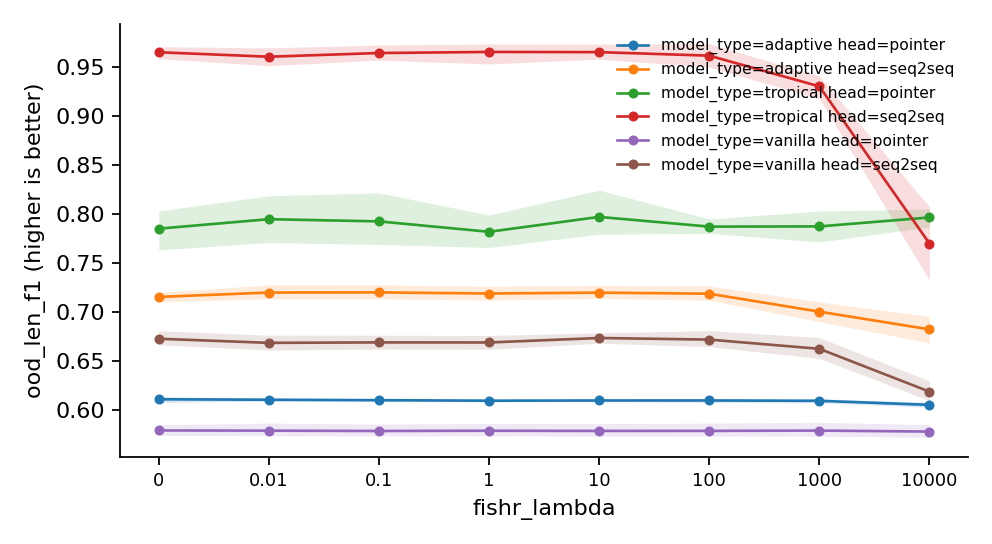
\includegraphics[width=\textwidth]{metric_ood_len_f1.png}
\caption{\texttt{ood\_len\_f1} against \texttt{fishr\_lambda}: the mean over seeds with a 95\% bootstrap CI, one line per combination of the other factors.}
\label{fig:ood_len_f1}
\end{figure}

{\small
\begin{longtable}{lllrlrrr}
\caption{\texttt{ood\_len\_f1} per cell: mean, 95\% bootstrap CI, SD, seeds, diverged runs.}\label{tab:summary-ood_len_f1}\\
\toprule
\texttt{model\_type} & \texttt{head} & \texttt{fishr\_lambda} & mean & 95\% CI & SD & $n$ & div.\\
\midrule
\endhead
adaptive & pointer & 0 & 0.6112 & [0.608, 0.614] & 0.0044 & 5 & 0\\
adaptive & pointer & 0.01 & 0.6107 & [0.609, 0.612] & 0.00211 & 5 & 0\\
adaptive & pointer & 0.1 & 0.6102 & [0.609, 0.612] & 0.00201 & 5 & 0\\
adaptive & pointer & 1 & 0.6097 & [0.608, 0.611] & 0.00159 & 5 & 0\\
adaptive & pointer & 10 & 0.6099 & [0.609, 0.611] & 0.0016 & 5 & 0\\
adaptive & pointer & 100 & 0.61 & [0.608, 0.612] & 0.00263 & 5 & 0\\
adaptive & pointer & 1000 & 0.6096 & [0.608, 0.612] & 0.00264 & 5 & 0\\
adaptive & pointer & 1e+04 & 0.6055 & [0.603, 0.608] & 0.00355 & 5 & 0\\
adaptive & seq2seq & 0 & 0.7155 & [0.711, 0.72] & 0.00602 & 5 & 0\\
adaptive & seq2seq & 0.01 & 0.7199 & [0.713, 0.728] & 0.00931 & 5 & 0\\
adaptive & seq2seq & 0.1 & 0.7201 & [0.714, 0.728] & 0.00926 & 5 & 0\\
adaptive & seq2seq & 1 & 0.7189 & [0.712, 0.726] & 0.00869 & 5 & 0\\
adaptive & seq2seq & 10 & 0.7198 & [0.714, 0.727] & 0.00822 & 5 & 0\\
adaptive & seq2seq & 100 & 0.7188 & [0.712, 0.727] & 0.00893 & 5 & 0\\
adaptive & seq2seq & 1000 & 0.7004 & [0.69, 0.71] & 0.0131 & 5 & 0\\
adaptive & seq2seq & 1e+04 & 0.6824 & [0.669, 0.696] & 0.0174 & 5 & 0\\
tropical & pointer & 0 & 0.785 & [0.763, 0.803] & 0.0271 & 5 & 0\\
tropical & pointer & 0.01 & 0.7947 & [0.771, 0.819] & 0.0302 & 5 & 0\\
tropical & pointer & 0.1 & 0.7924 & [0.769, 0.821] & 0.0335 & 5 & 0\\
tropical & pointer & 1 & 0.7818 & [0.766, 0.799] & 0.0231 & 5 & 0\\
tropical & pointer & 10 & 0.797 & [0.779, 0.824] & 0.0305 & 5 & 0\\
tropical & pointer & 100 & 0.7871 & [0.78, 0.795] & 0.0101 & 5 & 0\\
tropical & pointer & 1000 & 0.7873 & [0.771, 0.803] & 0.022 & 5 & 0\\
tropical & pointer & 1e+04 & 0.7964 & [0.787, 0.805] & 0.0112 & 5 & 0\\
tropical & seq2seq & 0 & 0.9648 & [0.958, 0.97] & 0.0078 & 5 & 0\\
tropical & seq2seq & 0.01 & 0.9602 & [0.951, 0.969] & 0.012 & 5 & 0\\
tropical & seq2seq & 0.1 & 0.964 & [0.957, 0.972] & 0.0102 & 5 & 0\\
tropical & seq2seq & 1 & 0.9651 & [0.953, 0.973] & 0.0136 & 5 & 0\\
tropical & seq2seq & 10 & 0.9649 & [0.958, 0.973] & 0.0101 & 5 & 0\\
tropical & seq2seq & 100 & 0.9613 & [0.95, 0.973] & 0.015 & 5 & 0\\
tropical & seq2seq & 1000 & 0.93 & [0.917, 0.94] & 0.0141 & 5 & 0\\
tropical & seq2seq & 1e+04 & 0.7699 & [0.732, 0.807] & 0.0501 & 5 & 0\\
vanilla & pointer & 0 & 0.5794 & [0.574, 0.585] & 0.00748 & 5 & 0\\
vanilla & pointer & 0.01 & 0.5792 & [0.574, 0.587] & 0.0086 & 5 & 0\\
vanilla & pointer & 0.1 & 0.5789 & [0.574, 0.586] & 0.00795 & 5 & 0\\
vanilla & pointer & 1 & 0.5791 & [0.574, 0.587] & 0.00842 & 5 & 0\\
vanilla & pointer & 10 & 0.5789 & [0.574, 0.586] & 0.00827 & 5 & 0\\
vanilla & pointer & 100 & 0.579 & [0.574, 0.587] & 0.00879 & 5 & 0\\
vanilla & pointer & 1000 & 0.5793 & [0.574, 0.588] & 0.00945 & 5 & 0\\
vanilla & pointer & 1e+04 & 0.5783 & [0.572, 0.585] & 0.00838 & 5 & 0\\
vanilla & seq2seq & 0 & 0.6728 & [0.667, 0.681] & 0.00953 & 5 & 0\\
vanilla & seq2seq & 0.01 & 0.6687 & [0.661, 0.676] & 0.01 & 5 & 0\\
vanilla & seq2seq & 0.1 & 0.6691 & [0.662, 0.676] & 0.00946 & 5 & 0\\
vanilla & seq2seq & 1 & 0.6691 & [0.662, 0.676] & 0.00966 & 5 & 0\\
vanilla & seq2seq & 10 & 0.6736 & [0.668, 0.679] & 0.007 & 5 & 0\\
vanilla & seq2seq & 100 & 0.672 & [0.665, 0.681] & 0.0101 & 5 & 0\\
vanilla & seq2seq & 1000 & 0.6626 & [0.653, 0.674] & 0.0133 & 5 & 0\\
vanilla & seq2seq & 1e+04 & 0.619 & [0.61, 0.63] & 0.013 & 5 & 0\\
\bottomrule
\end{longtable}
}

{\small
\begin{longtable}{lllrrrl}
\caption{\texttt{ood\_len\_f1}: each level of \texttt{fishr\_lambda} against its control (0), within each combination of the other factors. parametric: Dunnett vs control.}\label{tab:control-ood_len_f1}\\
\toprule
\texttt{model\_type} & \texttt{head} & \texttt{fishr\_lambda} & difference & 95\% CI & $p$ & \\
\midrule
\endhead
adaptive & pointer & 0.01 & $-4.625\times10^{-4}$ & [-0.00522, 0.0043] & 0.9999 & \\
adaptive & pointer & 0.1 & $-9.339\times10^{-4}$ & [-0.0057, 0.00383] & 0.9926 & \\
adaptive & pointer & 1 & -0.001433 & [-0.0062, 0.00333] & 0.9325 & \\
adaptive & pointer & 10 & -0.00124 & [-0.006, 0.00352] & 0.9660 & \\
adaptive & pointer & 100 & -0.001202 & [-0.00596, 0.00356] & 0.9709 & \\
adaptive & pointer & 1000 & -0.00157 & [-0.00633, 0.00319] & 0.8996 & \\
adaptive & pointer & 1e+04 & -0.005681 & [-0.0104, $-9.19\times10^{-4}$] & 0.0140 & *\\
adaptive & seq2seq & 0.01 & 0.004473 & [-0.0141, 0.0231] & 0.9774 & \\
adaptive & seq2seq & 0.1 & 0.004621 & [-0.014, 0.0232] & 0.9732 & \\
adaptive & seq2seq & 1 & 0.003468 & [-0.0151, 0.0221] & 0.9945 & \\
adaptive & seq2seq & 10 & 0.004375 & [-0.0142, 0.023] & 0.9798 & \\
adaptive & seq2seq & 100 & 0.003281 & [-0.0153, 0.0219] & 0.9960 & \\
adaptive & seq2seq & 1000 & -0.01503 & [-0.0336, 0.00357] & 0.1540 & \\
adaptive & seq2seq & 1e+04 & -0.03302 & [-0.0516, -0.0144] & 0.0002 & *\\
tropical & pointer & 0.01 & 0.00963 & [-0.0338, 0.0531] & 0.9854 & \\
tropical & pointer & 0.1 & 0.007389 & [-0.0361, 0.0508] & 0.9968 & \\
tropical & pointer & 1 & -0.003213 & [-0.0467, 0.0402] & 1.0000 & \\
tropical & pointer & 10 & 0.01198 & [-0.0315, 0.0554] & 0.9551 & \\
tropical & pointer & 100 & 0.002062 & [-0.0414, 0.0455] & 1.0000 & \\
tropical & pointer & 1000 & 0.00227 & [-0.0412, 0.0457] & 1.0000 & \\
tropical & pointer & 1e+04 & 0.01139 & [-0.0321, 0.0548] & 0.9648 & \\
tropical & seq2seq & 0.01 & -0.004555 & [-0.0412, 0.0321] & 0.9996 & \\
tropical & seq2seq & 0.1 & $-7.782\times10^{-4}$ & [-0.0374, 0.0359] & 1.0000 & \\
tropical & seq2seq & 1 & $3.253\times10^{-4}$ & [-0.0363, 0.037] & 1.0000 & \\
tropical & seq2seq & 10 & $1.233\times10^{-4}$ & [-0.0365, 0.0368] & 1.0000 & \\
tropical & seq2seq & 100 & -0.003478 & [-0.0401, 0.0332] & 0.9999 & \\
tropical & seq2seq & 1000 & -0.03478 & [-0.0715, 0.00189] & 0.0687 & \\
tropical & seq2seq & 1e+04 & -0.1949 & [-0.232, -0.158] & $<10^{-4}$ & *\\
vanilla & pointer & 0.01 & $-2.280\times10^{-4}$ & [-0.015, 0.0145] & 1.0000 & \\
vanilla & pointer & 0.1 & $-5.537\times10^{-4}$ & [-0.0153, 0.0142] & 1.0000 & \\
vanilla & pointer & 1 & $-2.986\times10^{-4}$ & [-0.015, 0.0144] & 1.0000 & \\
vanilla & pointer & 10 & $-5.047\times10^{-4}$ & [-0.0152, 0.0142] & 1.0000 & \\
vanilla & pointer & 100 & $-4.481\times10^{-4}$ & [-0.0152, 0.0143] & 1.0000 & \\
vanilla & pointer & 1000 & $-1.444\times10^{-4}$ & [-0.0149, 0.0146] & 1.0000 & \\
vanilla & pointer & 1e+04 & -0.001157 & [-0.0159, 0.0136] & 1.0000 & \\
vanilla & seq2seq & 0.01 & -0.004168 & [-0.0224, 0.0141] & 0.9827 & \\
vanilla & seq2seq & 0.1 & -0.003708 & [-0.0219, 0.0145] & 0.9909 & \\
vanilla & seq2seq & 1 & -0.003778 & [-0.022, 0.0145] & 0.9899 & \\
vanilla & seq2seq & 10 & $7.772\times10^{-4}$ & [-0.0175, 0.019] & 1.0000 & \\
vanilla & seq2seq & 100 & $-8.447\times10^{-4}$ & [-0.0191, 0.0174] & 1.0000 & \\
vanilla & seq2seq & 1000 & -0.01026 & [-0.0285, 0.00798] & 0.4821 & \\
vanilla & seq2seq & 1e+04 & -0.05389 & [-0.0721, -0.0357] & $<10^{-4}$ & *\\
\bottomrule
\end{longtable}
}

{\small
\begin{longtable}{llrrrrr}
\caption{\texttt{ood\_len\_f1} against log10 \texttt{fishr\_lambda}: parametric: OLS slope t-test, seed-bootstrap CI, with the Jonckheere--Terpstra ordered-trend $\tau$ and $p$.}\label{tab:trend-ood_len_f1}\\
\toprule
\texttt{model\_type} & \texttt{head} & estimate & 95\% CI & $p$ & JT $\tau$ & JT $p$\\
\midrule
\endhead
adaptive & pointer & $-5.964\times10^{-4}$ & [$-8.24\times10^{-4}$, $-4.04\times10^{-4}$] & 0.0076 & -0.326 & 0.0144\\
adaptive & seq2seq & -0.005428 & [-0.00711, -0.00375] & $<10^{-4}$ & -0.501 & 0.0002\\
tropical & pointer & $1.169\times10^{-5}$ & [-0.00302, 0.00303] & 0.9953 & 0.131 & 0.3229\\
tropical & seq2seq & -0.02296 & [-0.0269, -0.019] & $<10^{-4}$ & -0.512 & 0.0002\\
vanilla & pointer & $-7.560\times10^{-5}$ & [$-2.54\times10^{-4}$, $1.20\times10^{-4}$] & 0.9105 & -0.0552 & 0.6897\\
vanilla & seq2seq & -0.00569 & [-0.00744, -0.00393] & 0.0004 & -0.291 & 0.0266\\
\bottomrule
\end{longtable}
}

{\small
\begin{longtable}{lrrrl}
\caption{\texttt{ood\_len\_f1}: paired contrasts by seed, Holm-corrected across the cells. parametric: paired t-test by seed, Holm.}\label{tab:paired-ood_len_f1}\\
\toprule
contrast (within) & difference & 95\% CI & $p$ & \\
\midrule
\endhead
\stackcell{model\_type: tropical - vanilla\\\footnotesize head=pointer fishr\_lambda=0 } & 0.2056 & [0.167, 0.244] & 0.0005 & *\\
\stackcell{model\_type: tropical - vanilla\\\footnotesize head=pointer fishr\_lambda=0.01 } & 0.2155 & [0.181, 0.25] & 0.0003 & *\\
\stackcell{model\_type: tropical - vanilla\\\footnotesize head=pointer fishr\_lambda=0.1 } & 0.2135 & [0.171, 0.256] & 0.0005 & *\\
\stackcell{model\_type: tropical - vanilla\\\footnotesize head=pointer fishr\_lambda=1 } & 0.2027 & [0.172, 0.233] & 0.0003 & *\\
\stackcell{model\_type: tropical - vanilla\\\footnotesize head=pointer fishr\_lambda=10 } & 0.2181 & [0.175, 0.261] & 0.0005 & *\\
\stackcell{model\_type: tropical - vanilla\\\footnotesize head=pointer fishr\_lambda=100 } & 0.2081 & [0.187, 0.229] & $<10^{-4}$ & *\\
\stackcell{model\_type: tropical - vanilla\\\footnotesize head=pointer fishr\_lambda=1000 } & 0.208 & [0.179, 0.237] & 0.0003 & *\\
\stackcell{model\_type: tropical - vanilla\\\footnotesize head=pointer fishr\_lambda=1e+04 } & 0.2182 & [0.204, 0.233] & $<10^{-4}$ & *\\
\stackcell{model\_type: tropical - vanilla\\\footnotesize head=seq2seq fishr\_lambda=0 } & 0.2919 & [0.283, 0.301] & $<10^{-4}$ & *\\
\stackcell{model\_type: tropical - vanilla\\\footnotesize head=seq2seq fishr\_lambda=0.01 } & 0.2915 & [0.265, 0.318] & $<10^{-4}$ & *\\
\stackcell{model\_type: tropical - vanilla\\\footnotesize head=seq2seq fishr\_lambda=0.1 } & 0.2948 & [0.274, 0.316] & $<10^{-4}$ & *\\
\stackcell{model\_type: tropical - vanilla\\\footnotesize head=seq2seq fishr\_lambda=1 } & 0.296 & [0.269, 0.323] & $<10^{-4}$ & *\\
\stackcell{model\_type: tropical - vanilla\\\footnotesize head=seq2seq fishr\_lambda=10 } & 0.2913 & [0.277, 0.306] & $<10^{-4}$ & *\\
\stackcell{model\_type: tropical - vanilla\\\footnotesize head=seq2seq fishr\_lambda=100 } & 0.2893 & [0.266, 0.312] & $<10^{-4}$ & *\\
\stackcell{model\_type: tropical - vanilla\\\footnotesize head=seq2seq fishr\_lambda=1000 } & 0.2674 & [0.245, 0.29] & $<10^{-4}$ & *\\
\stackcell{model\_type: tropical - vanilla\\\footnotesize head=seq2seq fishr\_lambda=1e+04 } & 0.1509 & [0.102, 0.2] & 0.0010 & *\\
\stackcell{model\_type: adaptive - vanilla\\\footnotesize head=pointer fishr\_lambda=0 } & 0.03175 & [0.0185, 0.045] & 0.0108 & *\\
\stackcell{model\_type: adaptive - vanilla\\\footnotesize head=pointer fishr\_lambda=0.01 } & 0.03151 & [0.0203, 0.0427] & 0.0108 & *\\
\stackcell{model\_type: adaptive - vanilla\\\footnotesize head=pointer fishr\_lambda=0.1 } & 0.03137 & [0.0214, 0.0413] & 0.0094 & *\\
\stackcell{model\_type: adaptive - vanilla\\\footnotesize head=pointer fishr\_lambda=1 } & 0.03061 & [0.0203, 0.041] & 0.0108 & *\\
\stackcell{model\_type: adaptive - vanilla\\\footnotesize head=pointer fishr\_lambda=10 } & 0.03101 & [0.0205, 0.0415] & 0.0108 & *\\
\stackcell{model\_type: adaptive - vanilla\\\footnotesize head=pointer fishr\_lambda=100 } & 0.03099 & [0.0195, 0.0425] & 0.0108 & *\\
\stackcell{model\_type: adaptive - vanilla\\\footnotesize head=pointer fishr\_lambda=1000 } & 0.03032 & [0.018, 0.0427] & 0.0108 & *\\
\stackcell{model\_type: adaptive - vanilla\\\footnotesize head=pointer fishr\_lambda=1e+04 } & 0.02722 & [0.0152, 0.0392] & 0.0108 & *\\
\stackcell{model\_type: adaptive - vanilla\\\footnotesize head=seq2seq fishr\_lambda=0 } & 0.04262 & [0.0323, 0.053] & 0.0040 & *\\
\stackcell{model\_type: adaptive - vanilla\\\footnotesize head=seq2seq fishr\_lambda=0.01 } & 0.05127 & [0.0393, 0.0632] & 0.0040 & *\\
\stackcell{model\_type: adaptive - vanilla\\\footnotesize head=seq2seq fishr\_lambda=0.1 } & 0.05095 & [0.0388, 0.0632] & 0.0040 & *\\
\stackcell{model\_type: adaptive - vanilla\\\footnotesize head=seq2seq fishr\_lambda=1 } & 0.04987 & [0.038, 0.0617] & 0.0040 & *\\
\stackcell{model\_type: adaptive - vanilla\\\footnotesize head=seq2seq fishr\_lambda=10 } & 0.04622 & [0.0377, 0.0548] & 0.0018 & *\\
\stackcell{model\_type: adaptive - vanilla\\\footnotesize head=seq2seq fishr\_lambda=100 } & 0.04675 & [0.0363, 0.0572] & 0.0036 & *\\
\stackcell{model\_type: adaptive - vanilla\\\footnotesize head=seq2seq fishr\_lambda=1000 } & 0.03785 & [0.025, 0.0507] & 0.0108 & *\\
\stackcell{model\_type: adaptive - vanilla\\\footnotesize head=seq2seq fishr\_lambda=1e+04 } & 0.06349 & [0.0398, 0.0872] & 0.0108 & *\\
\stackcell{head: pointer - seq2seq\\\footnotesize model\_type=adaptive fishr\_lambda=0 } & -0.1043 & [-0.11, -0.0987] & $<10^{-4}$ & *\\
\stackcell{head: pointer - seq2seq\\\footnotesize model\_type=adaptive fishr\_lambda=0.01 } & -0.1092 & [-0.118, -0.1] & $<10^{-4}$ & *\\
\stackcell{head: pointer - seq2seq\\\footnotesize model\_type=adaptive fishr\_lambda=0.1 } & -0.1098 & [-0.119, -0.101] & 0.0001 & *\\
\stackcell{head: pointer - seq2seq\\\footnotesize model\_type=adaptive fishr\_lambda=1 } & -0.1092 & [-0.119, -0.0993] & 0.0001 & *\\
\stackcell{head: pointer - seq2seq\\\footnotesize model\_type=adaptive fishr\_lambda=10 } & -0.1099 & [-0.119, -0.101] & $<10^{-4}$ & *\\
\stackcell{head: pointer - seq2seq\\\footnotesize model\_type=adaptive fishr\_lambda=100 } & -0.1088 & [-0.117, -0.1] & $<10^{-4}$ & *\\
\stackcell{head: pointer - seq2seq\\\footnotesize model\_type=adaptive fishr\_lambda=1000 } & -0.09083 & [-0.104, -0.0775] & 0.0008 & *\\
\stackcell{head: pointer - seq2seq\\\footnotesize model\_type=adaptive fishr\_lambda=1e+04 } & -0.07695 & [-0.0949, -0.0589] & 0.0021 & *\\
\stackcell{head: pointer - seq2seq\\\footnotesize model\_type=tropical fishr\_lambda=0 } & -0.1797 & [-0.213, -0.147] & 0.0014 & *\\
\stackcell{head: pointer - seq2seq\\\footnotesize model\_type=tropical fishr\_lambda=0.01 } & -0.1655 & [-0.202, -0.129] & 0.0021 & *\\
\stackcell{head: pointer - seq2seq\\\footnotesize model\_type=tropical fishr\_lambda=0.1 } & -0.1716 & [-0.212, -0.131] & 0.0021 & *\\
\stackcell{head: pointer - seq2seq\\\footnotesize model\_type=tropical fishr\_lambda=1 } & -0.1833 & [-0.208, -0.159] & 0.0006 & *\\
\stackcell{head: pointer - seq2seq\\\footnotesize model\_type=tropical fishr\_lambda=10 } & -0.1679 & [-0.214, -0.122] & 0.0027 & *\\
\stackcell{head: pointer - seq2seq\\\footnotesize model\_type=tropical fishr\_lambda=100 } & -0.1742 & [-0.202, -0.146] & 0.0010 & *\\
\stackcell{head: pointer - seq2seq\\\footnotesize model\_type=tropical fishr\_lambda=1000 } & -0.1427 & [-0.182, -0.104] & 0.0027 & *\\
\stackcell{head: pointer - seq2seq\\\footnotesize model\_type=tropical fishr\_lambda=1e+04 } & 0.02655 & [-0.0383, 0.0914] & 0.3193 & \\
\stackcell{head: pointer - seq2seq\\\footnotesize model\_type=vanilla fishr\_lambda=0 } & -0.09341 & [-0.108, -0.0786] & 0.0010 & *\\
\stackcell{head: pointer - seq2seq\\\footnotesize model\_type=vanilla fishr\_lambda=0.01 } & -0.08947 & [-0.11, -0.0693] & 0.0021 & *\\
\stackcell{head: pointer - seq2seq\\\footnotesize model\_type=vanilla fishr\_lambda=0.1 } & -0.09026 & [-0.109, -0.0718] & 0.0020 & *\\
\stackcell{head: pointer - seq2seq\\\footnotesize model\_type=vanilla fishr\_lambda=1 } & -0.08993 & [-0.109, -0.0706] & 0.0021 & *\\
\stackcell{head: pointer - seq2seq\\\footnotesize model\_type=vanilla fishr\_lambda=10 } & -0.09469 & [-0.111, -0.0788] & 0.0011 & *\\
\stackcell{head: pointer - seq2seq\\\footnotesize model\_type=vanilla fishr\_lambda=100 } & -0.09301 & [-0.113, -0.0735] & 0.0021 & *\\
\stackcell{head: pointer - seq2seq\\\footnotesize model\_type=vanilla fishr\_lambda=1000 } & -0.0833 & [-0.107, -0.0595] & 0.0027 & *\\
\stackcell{head: pointer - seq2seq\\\footnotesize model\_type=vanilla fishr\_lambda=1e+04 } & -0.04068 & [-0.059, -0.0224] & 0.0070 & *\\
\bottomrule
\end{longtable}
}

\clearpage
\appendix
\section{Other metrics}
\subsection{\texttt{ood\_len\_exact}}
\begin{figure}[tbp]
\centering
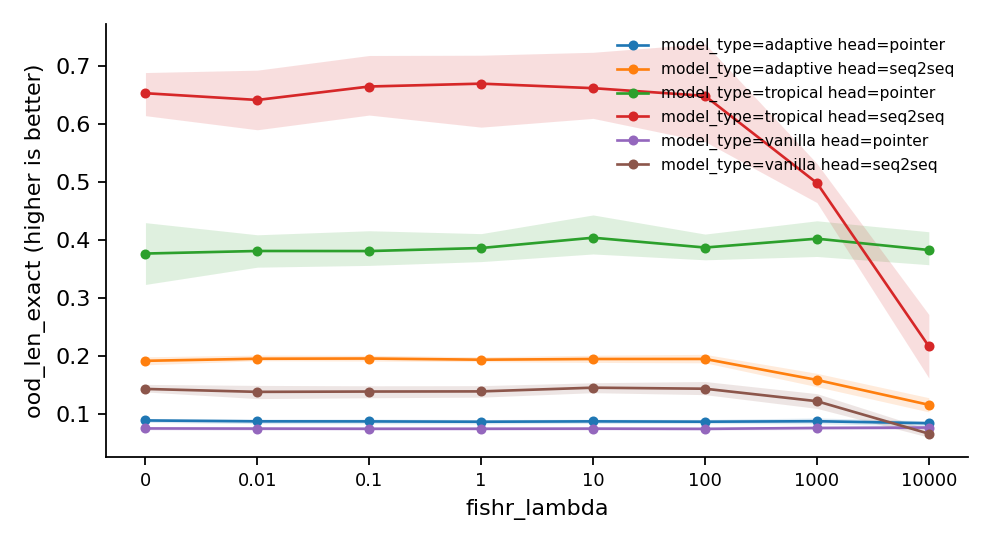
\includegraphics[width=\textwidth]{metric_ood_len_exact.png}
\caption{\texttt{ood\_len\_exact} against \texttt{fishr\_lambda}: the mean over seeds with a 95\% bootstrap CI, one line per combination of the other factors.}
\label{fig:ood_len_exact}
\end{figure}

{\small
\begin{longtable}{lllrlrrr}
\caption{\texttt{ood\_len\_exact} per cell: mean, 95\% bootstrap CI, SD, seeds, diverged runs.}\label{tab:summary-ood_len_exact}\\
\toprule
\texttt{model\_type} & \texttt{head} & \texttt{fishr\_lambda} & mean & 95\% CI & SD & $n$ & div.\\
\midrule
\endhead
adaptive & pointer & 0 & 0.08807 & [0.0847, 0.0914] & 0.00475 & 5 & 0\\
adaptive & pointer & 0.01 & 0.08653 & [0.0825, 0.0905] & 0.00527 & 5 & 0\\
adaptive & pointer & 0.1 & 0.08643 & [0.0823, 0.0905] & 0.00537 & 5 & 0\\
adaptive & pointer & 1 & 0.08587 & [0.082, 0.0897] & 0.00498 & 5 & 0\\
adaptive & pointer & 10 & 0.0865 & [0.0828, 0.0902] & 0.00474 & 5 & 0\\
adaptive & pointer & 100 & 0.08593 & [0.0824, 0.0898] & 0.00474 & 5 & 0\\
adaptive & pointer & 1000 & 0.08673 & [0.0823, 0.0924] & 0.00634 & 5 & 0\\
adaptive & pointer & 1e+04 & 0.0833 & [0.0789, 0.0875] & 0.00563 & 5 & 0\\
adaptive & seq2seq & 0 & 0.1912 & [0.184, 0.198] & 0.00884 & 5 & 0\\
adaptive & seq2seq & 0.01 & 0.1948 & [0.191, 0.201] & 0.00687 & 5 & 0\\
adaptive & seq2seq & 0.1 & 0.1951 & [0.191, 0.201] & 0.00659 & 5 & 0\\
adaptive & seq2seq & 1 & 0.1931 & [0.19, 0.198] & 0.00567 & 5 & 0\\
adaptive & seq2seq & 10 & 0.1943 & [0.188, 0.201] & 0.0077 & 5 & 0\\
adaptive & seq2seq & 100 & 0.1944 & [0.188, 0.202] & 0.00953 & 5 & 0\\
adaptive & seq2seq & 1000 & 0.1581 & [0.146, 0.17] & 0.0152 & 5 & 0\\
adaptive & seq2seq & 1e+04 & 0.1151 & [0.103, 0.127] & 0.0159 & 5 & 0\\
tropical & pointer & 0 & 0.3766 & [0.323, 0.43] & 0.0697 & 5 & 0\\
tropical & pointer & 0.01 & 0.381 & [0.353, 0.409] & 0.0364 & 5 & 0\\
tropical & pointer & 0.1 & 0.3809 & [0.356, 0.416] & 0.039 & 5 & 0\\
tropical & pointer & 1 & 0.3862 & [0.363, 0.411] & 0.0355 & 5 & 0\\
tropical & pointer & 10 & 0.404 & [0.376, 0.443] & 0.0444 & 5 & 0\\
tropical & pointer & 100 & 0.387 & [0.366, 0.41] & 0.0291 & 5 & 0\\
tropical & pointer & 1000 & 0.4023 & [0.372, 0.433] & 0.0409 & 5 & 0\\
tropical & pointer & 1e+04 & 0.3827 & [0.357, 0.414] & 0.0384 & 5 & 0\\
tropical & seq2seq & 0 & 0.6538 & [0.615, 0.69] & 0.0489 & 5 & 0\\
tropical & seq2seq & 0.01 & 0.6421 & [0.591, 0.694] & 0.0703 & 5 & 0\\
tropical & seq2seq & 0.1 & 0.6654 & [0.616, 0.719] & 0.0679 & 5 & 0\\
tropical & seq2seq & 1 & 0.6703 & [0.595, 0.719] & 0.0827 & 5 & 0\\
tropical & seq2seq & 10 & 0.6625 & [0.61, 0.725] & 0.0738 & 5 & 0\\
tropical & seq2seq & 100 & 0.6492 & [0.57, 0.739] & 0.106 & 5 & 0\\
tropical & seq2seq & 1000 & 0.4986 & [0.465, 0.532] & 0.0436 & 5 & 0\\
tropical & seq2seq & 1e+04 & 0.2163 & [0.162, 0.271] & 0.0735 & 5 & 0\\
vanilla & pointer & 0 & 0.07427 & [0.0718, 0.0763] & 0.00284 & 5 & 0\\
vanilla & pointer & 0.01 & 0.074 & [0.0711, 0.0763] & 0.00335 & 5 & 0\\
vanilla & pointer & 0.1 & 0.07373 & [0.0712, 0.0759] & 0.00309 & 5 & 0\\
vanilla & pointer & 1 & 0.07373 & [0.0712, 0.0763] & 0.00314 & 5 & 0\\
vanilla & pointer & 10 & 0.07397 & [0.0713, 0.0761] & 0.00321 & 5 & 0\\
vanilla & pointer & 100 & 0.07357 & [0.0712, 0.0761] & 0.00296 & 5 & 0\\
vanilla & pointer & 1000 & 0.0751 & [0.0723, 0.0779] & 0.00338 & 5 & 0\\
vanilla & pointer & 1e+04 & 0.0758 & [0.0726, 0.0793] & 0.00462 & 5 & 0\\
vanilla & seq2seq & 0 & 0.1425 & [0.137, 0.15] & 0.00886 & 5 & 0\\
vanilla & seq2seq & 0.01 & 0.1375 & [0.126, 0.149] & 0.0149 & 5 & 0\\
vanilla & seq2seq & 0.1 & 0.1381 & [0.127, 0.148] & 0.0136 & 5 & 0\\
vanilla & seq2seq & 1 & 0.1383 & [0.128, 0.148] & 0.0136 & 5 & 0\\
vanilla & seq2seq & 10 & 0.1447 & [0.136, 0.153] & 0.0113 & 5 & 0\\
vanilla & seq2seq & 100 & 0.1429 & [0.133, 0.155] & 0.014 & 5 & 0\\
vanilla & seq2seq & 1000 & 0.1214 & [0.109, 0.134] & 0.0164 & 5 & 0\\
vanilla & seq2seq & 1e+04 & 0.06523 & [0.059, 0.0727] & 0.00864 & 5 & 0\\
\bottomrule
\end{longtable}
}

{\small
\begin{longtable}{lllrrrl}
\caption{\texttt{ood\_len\_exact}: each level of \texttt{fishr\_lambda} against its control (0), within each combination of the other factors. parametric: Dunnett vs control.}\label{tab:control-ood_len_exact}\\
\toprule
\texttt{model\_type} & \texttt{head} & \texttt{fishr\_lambda} & difference & 95\% CI & $p$ & \\
\midrule
\endhead
adaptive & pointer & 0.01 & -0.001533 & [-0.0107, 0.00764] & 0.9971 & \\
adaptive & pointer & 0.1 & -0.001633 & [-0.0108, 0.00754] & 0.9958 & \\
adaptive & pointer & 1 & -0.0022 & [-0.0114, 0.00698] & 0.9777 & \\
adaptive & pointer & 10 & -0.001567 & [-0.0107, 0.00761] & 0.9967 & \\
adaptive & pointer & 100 & -0.002133 & [-0.0113, 0.00704] & 0.9810 & \\
adaptive & pointer & 1000 & -0.001333 & [-0.0105, 0.00784] & 0.9988 & \\
adaptive & pointer & 1e+04 & -0.004767 & [-0.0139, 0.00441] & 0.5635 & \\
adaptive & seq2seq & 0.01 & 0.0036 & [-0.0142, 0.0214] & 0.9913 & \\
adaptive & seq2seq & 0.1 & 0.003967 & [-0.0139, 0.0218] & 0.9851 & \\
adaptive & seq2seq & 1 & 0.001933 & [-0.0159, 0.0198] & 0.9998 & \\
adaptive & seq2seq & 10 & 0.003133 & [-0.0147, 0.021] & 0.9961 & \\
adaptive & seq2seq & 100 & 0.003233 & [-0.0146, 0.0211] & 0.9953 & \\
adaptive & seq2seq & 1000 & -0.03307 & [-0.0509, -0.0152] & $<10^{-4}$ & *\\
adaptive & seq2seq & 1e+04 & -0.07603 & [-0.0939, -0.0582] & $<10^{-4}$ & *\\
tropical & pointer & 0.01 & 0.004433 & [-0.071, 0.0799] & 1.0000 & \\
tropical & pointer & 0.1 & 0.0043 & [-0.0712, 0.0798] & 1.0000 & \\
tropical & pointer & 1 & 0.009567 & [-0.0659, 0.085] & 0.9995 & \\
tropical & pointer & 10 & 0.02737 & [-0.0481, 0.103] & 0.8536 & \\
tropical & pointer & 100 & 0.0104 & [-0.0651, 0.0859] & 0.9991 & \\
tropical & pointer & 1000 & 0.0257 & [-0.0498, 0.101] & 0.8855 & \\
tropical & pointer & 1e+04 & 0.006133 & [-0.0693, 0.0816] & 1.0000 & \\
tropical & seq2seq & 0.01 & -0.01167 & [-0.139, 0.116] & 0.9999 & \\
tropical & seq2seq & 0.1 & 0.0116 & [-0.116, 0.139] & 0.9999 & \\
tropical & seq2seq & 1 & 0.01653 & [-0.111, 0.144] & 0.9994 & \\
tropical & seq2seq & 10 & 0.008733 & [-0.119, 0.136] & 1.0000 & \\
tropical & seq2seq & 100 & -0.004567 & [-0.132, 0.123] & 1.0000 & \\
tropical & seq2seq & 1000 & -0.1552 & [-0.283, -0.0276] & 0.0118 & *\\
tropical & seq2seq & 1e+04 & -0.4375 & [-0.565, -0.31] & $<10^{-4}$ & *\\
vanilla & pointer & 0.01 & $-2.667\times10^{-4}$ & [-0.00614, 0.00561] & 1.0000 & \\
vanilla & pointer & 0.1 & $-5.333\times10^{-4}$ & [-0.00641, 0.00534] & 0.9999 & \\
vanilla & pointer & 1 & $-5.333\times10^{-4}$ & [-0.00641, 0.00534] & 0.9999 & \\
vanilla & pointer & 10 & $-3.000\times10^{-4}$ & [-0.00618, 0.00558] & 1.0000 & \\
vanilla & pointer & 100 & $-7.000\times10^{-4}$ & [-0.00658, 0.00518] & 0.9997 & \\
vanilla & pointer & 1000 & $8.333\times10^{-4}$ & [-0.00504, 0.00671] & 0.9990 & \\
vanilla & pointer & 1e+04 & 0.001533 & [-0.00434, 0.00741] & 0.9657 & \\
vanilla & seq2seq & 0.01 & -0.005033 & [-0.0276, 0.0176] & 0.9849 & \\
vanilla & seq2seq & 0.1 & -0.004467 & [-0.0271, 0.0181] & 0.9923 & \\
vanilla & seq2seq & 1 & -0.004233 & [-0.0268, 0.0184] & 0.9943 & \\
vanilla & seq2seq & 10 & 0.0022 & [-0.0204, 0.0248] & 0.9999 & \\
vanilla & seq2seq & 100 & $4.000\times10^{-4}$ & [-0.0222, 0.023] & 1.0000 & \\
vanilla & seq2seq & 1000 & -0.02117 & [-0.0438, 0.00143] & 0.0737 & \\
vanilla & seq2seq & 1e+04 & -0.0773 & [-0.0999, -0.0547] & $<10^{-4}$ & *\\
\bottomrule
\end{longtable}
}

{\small
\begin{longtable}{llrrrrr}
\caption{\texttt{ood\_len\_exact} against log10 \texttt{fishr\_lambda}: parametric: OLS slope t-test, seed-bootstrap CI, with the Jonckheere--Terpstra ordered-trend $\tau$ and $p$.}\label{tab:trend-ood_len_exact}\\
\toprule
\texttt{model\_type} & \texttt{head} & estimate & 95\% CI & $p$ & JT $\tau$ & JT $p$\\
\midrule
\endhead
adaptive & pointer & $-3.226\times10^{-4}$ & [$-6.50\times10^{-4}$, $8.94\times10^{-5}$] & 0.4495 & -0.061 & 0.6573\\
adaptive & seq2seq & -0.01113 & [-0.013, -0.00928] & $<10^{-4}$ & -0.573 & 0.0002\\
tropical & pointer & 0.00174 & [$-1.75\times10^{-4}$, 0.00407] & 0.5713 & 0.145 & 0.2737\\
tropical & seq2seq & -0.05829 & [-0.0658, -0.05] & $<10^{-4}$ & -0.528 & 0.0002\\
vanilla & pointer & $2.845\times10^{-4}$ & [$8.33\times10^{-5}$, $5.04\times10^{-4}$] & 0.3019 & 0.0971 & 0.4767\\
vanilla & seq2seq & -0.00877 & [-0.0107, -0.00697] & $<10^{-4}$ & -0.356 & 0.0070\\
\bottomrule
\end{longtable}
}

{\small
\begin{longtable}{lrrrl}
\caption{\texttt{ood\_len\_exact}: paired contrasts by seed, Holm-corrected across the cells. parametric: paired t-test by seed, Holm.}\label{tab:paired-ood_len_exact}\\
\toprule
contrast (within) & difference & 95\% CI & $p$ & \\
\midrule
\endhead
\stackcell{model\_type: tropical - vanilla\\\footnotesize head=pointer fishr\_lambda=0 } & 0.3023 & [0.213, 0.392] & 0.0014 & *\\
\stackcell{model\_type: tropical - vanilla\\\footnotesize head=pointer fishr\_lambda=0.01 } & 0.307 & [0.26, 0.354] & 0.0007 & *\\
\stackcell{model\_type: tropical - vanilla\\\footnotesize head=pointer fishr\_lambda=0.1 } & 0.3072 & [0.256, 0.358] & 0.0007 & *\\
\stackcell{model\_type: tropical - vanilla\\\footnotesize head=pointer fishr\_lambda=1 } & 0.3124 & [0.266, 0.359] & 0.0007 & *\\
\stackcell{model\_type: tropical - vanilla\\\footnotesize head=pointer fishr\_lambda=10 } & 0.33 & [0.272, 0.388] & 0.0008 & *\\
\stackcell{model\_type: tropical - vanilla\\\footnotesize head=pointer fishr\_lambda=100 } & 0.3134 & [0.277, 0.35] & 0.0003 & *\\
\stackcell{model\_type: tropical - vanilla\\\footnotesize head=pointer fishr\_lambda=1000 } & 0.3272 & [0.275, 0.379] & 0.0007 & *\\
\stackcell{model\_type: tropical - vanilla\\\footnotesize head=pointer fishr\_lambda=1e+04 } & 0.3069 & [0.258, 0.356] & 0.0007 & *\\
\stackcell{model\_type: tropical - vanilla\\\footnotesize head=seq2seq fishr\_lambda=0 } & 0.5112 & [0.455, 0.567] & 0.0002 & *\\
\stackcell{model\_type: tropical - vanilla\\\footnotesize head=seq2seq fishr\_lambda=0.01 } & 0.5046 & [0.4, 0.609] & 0.0009 & *\\
\stackcell{model\_type: tropical - vanilla\\\footnotesize head=seq2seq fishr\_lambda=0.1 } & 0.5273 & [0.434, 0.621] & 0.0008 & *\\
\stackcell{model\_type: tropical - vanilla\\\footnotesize head=seq2seq fishr\_lambda=1 } & 0.532 & [0.419, 0.645] & 0.0009 & *\\
\stackcell{model\_type: tropical - vanilla\\\footnotesize head=seq2seq fishr\_lambda=10 } & 0.5178 & [0.425, 0.61] & 0.0008 & *\\
\stackcell{model\_type: tropical - vanilla\\\footnotesize head=seq2seq fishr\_lambda=100 } & 0.5063 & [0.374, 0.639] & 0.0013 & *\\
\stackcell{model\_type: tropical - vanilla\\\footnotesize head=seq2seq fishr\_lambda=1000 } & 0.3772 & [0.321, 0.433] & 0.0007 & *\\
\stackcell{model\_type: tropical - vanilla\\\footnotesize head=seq2seq fishr\_lambda=1e+04 } & 0.151 & [0.0652, 0.237] & 0.0081 & *\\
\stackcell{model\_type: adaptive - vanilla\\\footnotesize head=pointer fishr\_lambda=0 } & 0.0138 & [0.00713, 0.0205] & 0.0349 & *\\
\stackcell{model\_type: adaptive - vanilla\\\footnotesize head=pointer fishr\_lambda=0.01 } & 0.01253 & [0.0058, 0.0193] & 0.0349 & *\\
\stackcell{model\_type: adaptive - vanilla\\\footnotesize head=pointer fishr\_lambda=0.1 } & 0.0127 & [0.00656, 0.0188] & 0.0349 & *\\
\stackcell{model\_type: adaptive - vanilla\\\footnotesize head=pointer fishr\_lambda=1 } & 0.01213 & [0.00529, 0.019] & 0.0349 & *\\
\stackcell{model\_type: adaptive - vanilla\\\footnotesize head=pointer fishr\_lambda=10 } & 0.01253 & [0.00654, 0.0185] & 0.0349 & *\\
\stackcell{model\_type: adaptive - vanilla\\\footnotesize head=pointer fishr\_lambda=100 } & 0.01237 & [0.00511, 0.0196] & 0.0349 & *\\
\stackcell{model\_type: adaptive - vanilla\\\footnotesize head=pointer fishr\_lambda=1000 } & 0.01163 & [0.00174, 0.0215] & 0.0620 & \\
\stackcell{model\_type: adaptive - vanilla\\\footnotesize head=pointer fishr\_lambda=1e+04 } & 0.0075 & [$6.22\times10^{-4}$, 0.0144] & 0.0620 & \\
\stackcell{model\_type: adaptive - vanilla\\\footnotesize head=seq2seq fishr\_lambda=0 } & 0.04863 & [0.0391, 0.0581] & 0.0018 & *\\
\stackcell{model\_type: adaptive - vanilla\\\footnotesize head=seq2seq fishr\_lambda=0.01 } & 0.05727 & [0.0425, 0.0721] & 0.0047 & *\\
\stackcell{model\_type: adaptive - vanilla\\\footnotesize head=seq2seq fishr\_lambda=0.1 } & 0.05707 & [0.0417, 0.0724] & 0.0050 & *\\
\stackcell{model\_type: adaptive - vanilla\\\footnotesize head=seq2seq fishr\_lambda=1 } & 0.0548 & [0.042, 0.0676] & 0.0034 & *\\
\stackcell{model\_type: adaptive - vanilla\\\footnotesize head=seq2seq fishr\_lambda=10 } & 0.04957 & [0.0407, 0.0584] & 0.0015 & *\\
\stackcell{model\_type: adaptive - vanilla\\\footnotesize head=seq2seq fishr\_lambda=100 } & 0.05147 & [0.0449, 0.058] & 0.0004 & *\\
\stackcell{model\_type: adaptive - vanilla\\\footnotesize head=seq2seq fishr\_lambda=1000 } & 0.03673 & [0.03, 0.0435] & 0.0016 & *\\
\stackcell{model\_type: adaptive - vanilla\\\footnotesize head=seq2seq fishr\_lambda=1e+04 } & 0.0499 & [0.0312, 0.0686] & 0.0160 & *\\
\stackcell{head: pointer - seq2seq\\\footnotesize model\_type=adaptive fishr\_lambda=0 } & -0.1031 & [-0.113, -0.0934] & 0.0001 & *\\
\stackcell{head: pointer - seq2seq\\\footnotesize model\_type=adaptive fishr\_lambda=0.01 } & -0.1082 & [-0.113, -0.103] & $<10^{-4}$ & *\\
\stackcell{head: pointer - seq2seq\\\footnotesize model\_type=adaptive fishr\_lambda=0.1 } & -0.1087 & [-0.115, -0.102] & $<10^{-4}$ & *\\
\stackcell{head: pointer - seq2seq\\\footnotesize model\_type=adaptive fishr\_lambda=1 } & -0.1072 & [-0.111, -0.103] & $<10^{-4}$ & *\\
\stackcell{head: pointer - seq2seq\\\footnotesize model\_type=adaptive fishr\_lambda=10 } & -0.1078 & [-0.115, -0.101] & $<10^{-4}$ & *\\
\stackcell{head: pointer - seq2seq\\\footnotesize model\_type=adaptive fishr\_lambda=100 } & -0.1085 & [-0.115, -0.102] & $<10^{-4}$ & *\\
\stackcell{head: pointer - seq2seq\\\footnotesize model\_type=adaptive fishr\_lambda=1000 } & -0.07137 & [-0.084, -0.0587] & 0.0018 & *\\
\stackcell{head: pointer - seq2seq\\\footnotesize model\_type=adaptive fishr\_lambda=1e+04 } & -0.03183 & [-0.0472, -0.0164] & 0.0278 & *\\
\stackcell{head: pointer - seq2seq\\\footnotesize model\_type=tropical fishr\_lambda=0 } & -0.2772 & [-0.399, -0.155] & 0.0259 & *\\
\stackcell{head: pointer - seq2seq\\\footnotesize model\_type=tropical fishr\_lambda=0.01 } & -0.2611 & [-0.349, -0.174] & 0.0115 & *\\
\stackcell{head: pointer - seq2seq\\\footnotesize model\_type=tropical fishr\_lambda=0.1 } & -0.2845 & [-0.377, -0.192] & 0.0115 & *\\
\stackcell{head: pointer - seq2seq\\\footnotesize model\_type=tropical fishr\_lambda=1 } & -0.2841 & [-0.375, -0.193] & 0.0115 & *\\
\stackcell{head: pointer - seq2seq\\\footnotesize model\_type=tropical fishr\_lambda=10 } & -0.2585 & [-0.385, -0.132] & 0.0278 & *\\
\stackcell{head: pointer - seq2seq\\\footnotesize model\_type=tropical fishr\_lambda=100 } & -0.2622 & [-0.41, -0.114] & 0.0319 & *\\
\stackcell{head: pointer - seq2seq\\\footnotesize model\_type=tropical fishr\_lambda=1000 } & -0.09627 & [-0.178, -0.0141] & 0.0626 & \\
\stackcell{head: pointer - seq2seq\\\footnotesize model\_type=tropical fishr\_lambda=1e+04 } & 0.1665 & [0.0489, 0.284] & 0.0513 & \\
\stackcell{head: pointer - seq2seq\\\footnotesize model\_type=vanilla fishr\_lambda=0 } & -0.06827 & [-0.081, -0.0556] & 0.0020 & *\\
\stackcell{head: pointer - seq2seq\\\footnotesize model\_type=vanilla fishr\_lambda=0.01 } & -0.0635 & [-0.0843, -0.0427] & 0.0115 & *\\
\stackcell{head: pointer - seq2seq\\\footnotesize model\_type=vanilla fishr\_lambda=0.1 } & -0.06433 & [-0.0825, -0.0462] & 0.0083 & *\\
\stackcell{head: pointer - seq2seq\\\footnotesize model\_type=vanilla fishr\_lambda=1 } & -0.06457 & [-0.0834, -0.0458] & 0.0088 & *\\
\stackcell{head: pointer - seq2seq\\\footnotesize model\_type=vanilla fishr\_lambda=10 } & -0.07077 & [-0.0863, -0.0553] & 0.0036 & *\\
\stackcell{head: pointer - seq2seq\\\footnotesize model\_type=vanilla fishr\_lambda=100 } & -0.06937 & [-0.0883, -0.0505] & 0.0079 & *\\
\stackcell{head: pointer - seq2seq\\\footnotesize model\_type=vanilla fishr\_lambda=1000 } & -0.04627 & [-0.0678, -0.0247] & 0.0278 & *\\
\stackcell{head: pointer - seq2seq\\\footnotesize model\_type=vanilla fishr\_lambda=1e+04 } & 0.01057 & [-0.00355, 0.0247] & 0.1063 & \\
\bottomrule
\end{longtable}
}

\subsection{\texttt{ood\_val\_f1}}
\begin{figure}[tbp]
\centering
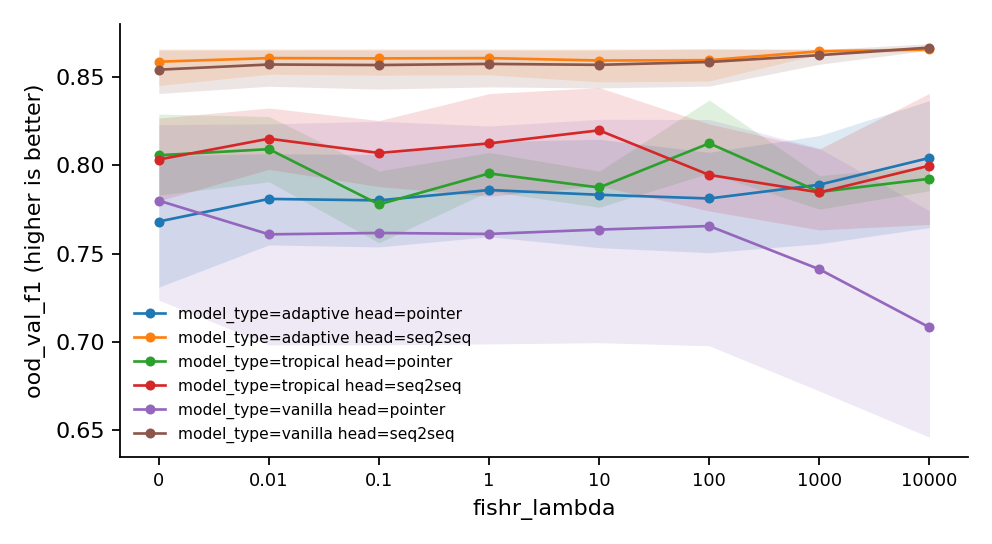
\includegraphics[width=\textwidth]{metric_ood_val_f1.png}
\caption{\texttt{ood\_val\_f1} against \texttt{fishr\_lambda}: the mean over seeds with a 95\% bootstrap CI, one line per combination of the other factors.}
\label{fig:ood_val_f1}
\end{figure}

{\small
\begin{longtable}{lllrlrrr}
\caption{\texttt{ood\_val\_f1} per cell: mean, 95\% bootstrap CI, SD, seeds, diverged runs.}\label{tab:summary-ood_val_f1}\\
\toprule
\texttt{model\_type} & \texttt{head} & \texttt{fishr\_lambda} & mean & 95\% CI & SD & $n$ & div.\\
\midrule
\endhead
adaptive & pointer & 0 & 0.7683 & [0.731, 0.805] & 0.0473 & 5 & 0\\
adaptive & pointer & 0.01 & 0.781 & [0.755, 0.807] & 0.0353 & 5 & 0\\
adaptive & pointer & 0.1 & 0.7802 & [0.754, 0.806] & 0.0362 & 5 & 0\\
adaptive & pointer & 1 & 0.7861 & [0.76, 0.814] & 0.0364 & 5 & 0\\
adaptive & pointer & 10 & 0.7834 & [0.753, 0.815] & 0.041 & 5 & 0\\
adaptive & pointer & 100 & 0.7813 & [0.751, 0.807] & 0.0359 & 5 & 0\\
adaptive & pointer & 1000 & 0.7891 & [0.756, 0.817] & 0.0394 & 5 & 0\\
adaptive & pointer & 1e+04 & 0.8043 & [0.765, 0.837] & 0.0459 & 5 & 0\\
adaptive & seq2seq & 0 & 0.8587 & [0.845, 0.866] & 0.015 & 5 & 0\\
adaptive & seq2seq & 0.01 & 0.8608 & [0.852, 0.866] & 0.0104 & 5 & 0\\
adaptive & seq2seq & 0.1 & 0.8606 & [0.851, 0.866] & 0.0108 & 5 & 0\\
adaptive & seq2seq & 1 & 0.8608 & [0.851, 0.866] & 0.0104 & 5 & 0\\
adaptive & seq2seq & 10 & 0.8594 & [0.847, 0.866] & 0.0135 & 5 & 0\\
adaptive & seq2seq & 100 & 0.8596 & [0.848, 0.866] & 0.0131 & 5 & 0\\
adaptive & seq2seq & 1000 & 0.8646 & [0.863, 0.866] & 0.00201 & 5 & 0\\
adaptive & seq2seq & 1e+04 & 0.8657 & [0.865, 0.866] & 0.00108 & 5 & 0\\
tropical & pointer & 0 & 0.8058 & [0.783, 0.829] & 0.0293 & 5 & 0\\
tropical & pointer & 0.01 & 0.8092 & [0.791, 0.828] & 0.0237 & 5 & 0\\
tropical & pointer & 0.1 & 0.778 & [0.756, 0.797] & 0.0259 & 5 & 0\\
tropical & pointer & 1 & 0.7955 & [0.785, 0.807] & 0.014 & 5 & 0\\
tropical & pointer & 10 & 0.7875 & [0.776, 0.797] & 0.0132 & 5 & 0\\
tropical & pointer & 100 & 0.8125 & [0.796, 0.837] & 0.0281 & 5 & 0\\
tropical & pointer & 1000 & 0.785 & [0.775, 0.794] & 0.0126 & 5 & 0\\
tropical & pointer & 1e+04 & 0.7925 & [0.786, 0.799] & 0.00889 & 5 & 0\\
tropical & seq2seq & 0 & 0.8033 & [0.78, 0.827] & 0.03 & 5 & 0\\
tropical & seq2seq & 0.01 & 0.8152 & [0.798, 0.833] & 0.0225 & 5 & 0\\
tropical & seq2seq & 0.1 & 0.8071 & [0.788, 0.825] & 0.0233 & 5 & 0\\
tropical & seq2seq & 1 & 0.8125 & [0.783, 0.841] & 0.0364 & 5 & 0\\
tropical & seq2seq & 10 & 0.8199 & [0.788, 0.844] & 0.0378 & 5 & 0\\
tropical & seq2seq & 100 & 0.7946 & [0.774, 0.823] & 0.0326 & 5 & 0\\
tropical & seq2seq & 1000 & 0.7847 & [0.763, 0.809] & 0.0303 & 5 & 0\\
tropical & seq2seq & 1e+04 & 0.7999 & [0.767, 0.841] & 0.0484 & 5 & 0\\
vanilla & pointer & 0 & 0.7801 & [0.724, 0.823] & 0.0661 & 5 & 0\\
vanilla & pointer & 0.01 & 0.761 & [0.698, 0.824] & 0.0841 & 5 & 0\\
vanilla & pointer & 0.1 & 0.7618 & [0.698, 0.825] & 0.0847 & 5 & 0\\
vanilla & pointer & 1 & 0.7612 & [0.699, 0.822] & 0.0836 & 5 & 0\\
vanilla & pointer & 10 & 0.7637 & [0.7, 0.826] & 0.0841 & 5 & 0\\
vanilla & pointer & 100 & 0.7657 & [0.698, 0.826] & 0.0826 & 5 & 0\\
vanilla & pointer & 1000 & 0.7412 & [0.672, 0.81] & 0.0856 & 5 & 0\\
vanilla & pointer & 1e+04 & 0.7083 & [0.646, 0.774] & 0.0829 & 5 & 0\\
vanilla & seq2seq & 0 & 0.8542 & [0.841, 0.865] & 0.0157 & 5 & 0\\
vanilla & seq2seq & 0.01 & 0.8572 & [0.845, 0.865] & 0.0143 & 5 & 0\\
vanilla & seq2seq & 0.1 & 0.8569 & [0.843, 0.865] & 0.015 & 5 & 0\\
vanilla & seq2seq & 1 & 0.8575 & [0.844, 0.865] & 0.0144 & 5 & 0\\
vanilla & seq2seq & 10 & 0.857 & [0.844, 0.865] & 0.0144 & 5 & 0\\
vanilla & seq2seq & 100 & 0.8586 & [0.845, 0.866] & 0.0151 & 5 & 0\\
vanilla & seq2seq & 1000 & 0.8624 & [0.857, 0.866] & 0.0058 & 5 & 0\\
vanilla & seq2seq & 1e+04 & 0.8667 & [0.865, 0.869] & 0.00245 & 5 & 0\\
\bottomrule
\end{longtable}
}

{\small
\begin{longtable}{lllrrrl}
\caption{\texttt{ood\_val\_f1}: each level of \texttt{fishr\_lambda} against its control (0), within each combination of the other factors. parametric: Dunnett vs control.}\label{tab:control-ood_val_f1}\\
\toprule
\texttt{model\_type} & \texttt{head} & \texttt{fishr\_lambda} & difference & 95\% CI & $p$ & \\
\midrule
\endhead
adaptive & pointer & 0.01 & 0.01279 & [-0.0569, 0.0825] & 0.9950 & \\
adaptive & pointer & 0.1 & 0.01197 & [-0.0578, 0.0817] & 0.9966 & \\
adaptive & pointer & 1 & 0.01782 & [-0.0519, 0.0875] & 0.9691 & \\
adaptive & pointer & 10 & 0.01514 & [-0.0546, 0.0849] & 0.9869 & \\
adaptive & pointer & 100 & 0.01303 & [-0.0567, 0.0828] & 0.9944 & \\
adaptive & pointer & 1000 & 0.02084 & [-0.0489, 0.0906] & 0.9344 & \\
adaptive & pointer & 1e+04 & 0.03602 & [-0.0337, 0.106] & 0.5690 & \\
adaptive & seq2seq & 0.01 & 0.002033 & [-0.0166, 0.0207] & 0.9998 & \\
adaptive & seq2seq & 0.1 & 0.001867 & [-0.0168, 0.0205] & 0.9999 & \\
adaptive & seq2seq & 1 & 0.002033 & [-0.0166, 0.0207] & 0.9998 & \\
adaptive & seq2seq & 10 & $6.730\times10^{-4}$ & [-0.018, 0.0193] & 1.0000 & \\
adaptive & seq2seq & 100 & $8.625\times10^{-4}$ & [-0.0178, 0.0195] & 1.0000 & \\
adaptive & seq2seq & 1000 & 0.005888 & [-0.0128, 0.0246] & 0.9169 & \\
adaptive & seq2seq & 1e+04 & 0.006912 & [-0.0118, 0.0256] & 0.8418 & \\
tropical & pointer & 0.01 & 0.003463 & [-0.033, 0.0399] & 0.9999 & \\
tropical & pointer & 0.1 & -0.02782 & [-0.0643, 0.00867] & 0.1956 & \\
tropical & pointer & 1 & -0.0103 & [-0.0468, 0.0262] & 0.9497 & \\
tropical & pointer & 10 & -0.01825 & [-0.0547, 0.0182] & 0.6007 & \\
tropical & pointer & 100 & 0.006763 & [-0.0297, 0.0432] & 0.9947 & \\
tropical & pointer & 1000 & -0.02078 & [-0.0573, 0.0157] & 0.4691 & \\
tropical & pointer & 1e+04 & -0.01329 & [-0.0498, 0.0232] & 0.8513 & \\
tropical & seq2seq & 0.01 & 0.01181 & [-0.0469, 0.0705] & 0.9914 & \\
tropical & seq2seq & 0.1 & 0.00371 & [-0.055, 0.0624] & 1.0000 & \\
tropical & seq2seq & 1 & 0.00915 & [-0.0495, 0.0678] & 0.9981 & \\
tropical & seq2seq & 10 & 0.01654 & [-0.0421, 0.0752] & 0.9500 & \\
tropical & seq2seq & 100 & -0.008729 & [-0.0674, 0.0499] & 0.9986 & \\
tropical & seq2seq & 1000 & -0.0186 & [-0.0773, 0.0401] & 0.9149 & \\
tropical & seq2seq & 1e+04 & -0.003446 & [-0.0621, 0.0552] & 1.0000 & \\
vanilla & pointer & 0.01 & -0.0191 & [-0.162, 0.124] & 0.9993 & \\
vanilla & pointer & 0.1 & -0.01832 & [-0.161, 0.125] & 0.9995 & \\
vanilla & pointer & 1 & -0.01887 & [-0.162, 0.124] & 0.9993 & \\
vanilla & pointer & 10 & -0.0164 & [-0.16, 0.127] & 0.9997 & \\
vanilla & pointer & 100 & -0.01439 & [-0.157, 0.129] & 0.9999 & \\
vanilla & pointer & 1000 & -0.03887 & [-0.182, 0.104] & 0.9582 & \\
vanilla & pointer & 1e+04 & -0.07179 & [-0.215, 0.0713] & 0.5981 & \\
vanilla & seq2seq & 0.01 & 0.00293 & [-0.0198, 0.0257] & 0.9994 & \\
vanilla & seq2seq & 0.1 & 0.002629 & [-0.0201, 0.0254] & 0.9997 & \\
vanilla & seq2seq & 1 & 0.003264 & [-0.0195, 0.026] & 0.9989 & \\
vanilla & seq2seq & 10 & 0.002737 & [-0.02, 0.0255] & 0.9996 & \\
vanilla & seq2seq & 100 & 0.004337 & [-0.0184, 0.0271] & 0.9937 & \\
vanilla & seq2seq & 1000 & 0.008207 & [-0.0146, 0.031] & 0.8568 & \\
vanilla & seq2seq & 1e+04 & 0.01251 & [-0.0103, 0.0353] & 0.5064 & \\
\bottomrule
\end{longtable}
}

{\small
\begin{longtable}{llrrrrr}
\caption{\texttt{ood\_val\_f1} against log10 \texttt{fishr\_lambda}: parametric: OLS slope t-test, seed-bootstrap CI, with the Jonckheere--Terpstra ordered-trend $\tau$ and $p$.}\label{tab:trend-ood_val_f1}\\
\toprule
\texttt{model\_type} & \texttt{head} & estimate & 95\% CI & $p$ & JT $\tau$ & JT $p$\\
\midrule
\endhead
adaptive & pointer & 0.002951 & [$8.05\times10^{-4}$, 0.00537] & 0.3401 & 0.139 & 0.3073\\
adaptive & seq2seq & $7.681\times10^{-4}$ & [$4.12\times10^{-7}$, 0.0023] & 0.3362 & 0.12 & 0.3833\\
tropical & pointer & $-6.826\times10^{-4}$ & [-0.00225, $5.55\times10^{-4}$] & 0.7097 & -0.0438 & 0.7485\\
tropical & seq2seq & -0.003867 & [-0.00978, 0.00199] & 0.1696 & -0.211 & 0.1082\\
vanilla & pointer & -0.006953 & [-0.00873, -0.00517] & 0.3025 & -0.109 & 0.4299\\
vanilla & seq2seq & 0.001463 & [$1.49\times10^{-4}$, 0.00332] & 0.1512 & 0.225 & 0.0892\\
\bottomrule
\end{longtable}
}

{\small
\begin{longtable}{lrrrl}
\caption{\texttt{ood\_val\_f1}: paired contrasts by seed, Holm-corrected across the cells. parametric: paired t-test by seed, Holm.}\label{tab:paired-ood_val_f1}\\
\toprule
contrast (within) & difference & 95\% CI & $p$ & \\
\midrule
\endhead
\stackcell{model\_type: tropical - vanilla\\\footnotesize head=pointer fishr\_lambda=0 } & 0.02568 & [-0.0432, 0.0945] & 1.0000 & \\
\stackcell{model\_type: tropical - vanilla\\\footnotesize head=pointer fishr\_lambda=0.01 } & 0.04824 & [-0.0515, 0.148] & 1.0000 & \\
\stackcell{model\_type: tropical - vanilla\\\footnotesize head=pointer fishr\_lambda=0.1 } & 0.01618 & [-0.0991, 0.131] & 1.0000 & \\
\stackcell{model\_type: tropical - vanilla\\\footnotesize head=pointer fishr\_lambda=1 } & 0.03425 & [-0.0612, 0.13] & 1.0000 & \\
\stackcell{model\_type: tropical - vanilla\\\footnotesize head=pointer fishr\_lambda=10 } & 0.02384 & [-0.084, 0.132] & 1.0000 & \\
\stackcell{model\_type: tropical - vanilla\\\footnotesize head=pointer fishr\_lambda=100 } & 0.04683 & [-0.0436, 0.137] & 1.0000 & \\
\stackcell{model\_type: tropical - vanilla\\\footnotesize head=pointer fishr\_lambda=1000 } & 0.04377 & [-0.0627, 0.15] & 1.0000 & \\
\stackcell{model\_type: tropical - vanilla\\\footnotesize head=pointer fishr\_lambda=1e+04 } & 0.08418 & [-0.0129, 0.181] & 0.6640 & \\
\stackcell{model\_type: tropical - vanilla\\\footnotesize head=seq2seq fishr\_lambda=0 } & -0.05089 & [-0.092, -0.00972] & 0.3177 & \\
\stackcell{model\_type: tropical - vanilla\\\footnotesize head=seq2seq fishr\_lambda=0.01 } & -0.042 & [-0.0705, -0.0135] & 0.1948 & \\
\stackcell{model\_type: tropical - vanilla\\\footnotesize head=seq2seq fishr\_lambda=0.1 } & -0.04981 & [-0.0814, -0.0182] & 0.1757 & \\
\stackcell{model\_type: tropical - vanilla\\\footnotesize head=seq2seq fishr\_lambda=1 } & -0.045 & [-0.0924, 0.00237] & 0.5772 & \\
\stackcell{model\_type: tropical - vanilla\\\footnotesize head=seq2seq fishr\_lambda=10 } & -0.03709 & [-0.0927, 0.0185] & 1.0000 & \\
\stackcell{model\_type: tropical - vanilla\\\footnotesize head=seq2seq fishr\_lambda=100 } & -0.06395 & [-0.104, -0.0236] & 0.1757 & \\
\stackcell{model\_type: tropical - vanilla\\\footnotesize head=seq2seq fishr\_lambda=1000 } & -0.0777 & [-0.118, -0.0377] & 0.0917 & \\
\stackcell{model\_type: tropical - vanilla\\\footnotesize head=seq2seq fishr\_lambda=1e+04 } & -0.06684 & [-0.127, -0.00622] & 0.4137 & \\
\stackcell{model\_type: adaptive - vanilla\\\footnotesize head=pointer fishr\_lambda=0 } & -0.01183 & [-0.0989, 0.0752] & 1.0000 & \\
\stackcell{model\_type: adaptive - vanilla\\\footnotesize head=pointer fishr\_lambda=0.01 } & 0.02006 & [-0.0887, 0.129] & 1.0000 & \\
\stackcell{model\_type: adaptive - vanilla\\\footnotesize head=pointer fishr\_lambda=0.1 } & 0.01846 & [-0.0931, 0.13] & 1.0000 & \\
\stackcell{model\_type: adaptive - vanilla\\\footnotesize head=pointer fishr\_lambda=1 } & 0.02486 & [-0.0866, 0.136] & 1.0000 & \\
\stackcell{model\_type: adaptive - vanilla\\\footnotesize head=pointer fishr\_lambda=10 } & 0.01971 & [-0.0935, 0.133] & 1.0000 & \\
\stackcell{model\_type: adaptive - vanilla\\\footnotesize head=pointer fishr\_lambda=100 } & 0.01559 & [-0.0959, 0.127] & 1.0000 & \\
\stackcell{model\_type: adaptive - vanilla\\\footnotesize head=pointer fishr\_lambda=1000 } & 0.04788 & [-0.0838, 0.18] & 1.0000 & \\
\stackcell{model\_type: adaptive - vanilla\\\footnotesize head=pointer fishr\_lambda=1e+04 } & 0.09597 & [-0.0281, 0.22] & 1.0000 & \\
\stackcell{model\_type: adaptive - vanilla\\\footnotesize head=seq2seq fishr\_lambda=0 } & 0.004512 & [-0.00746, 0.0165] & 1.0000 & \\
\stackcell{model\_type: adaptive - vanilla\\\footnotesize head=seq2seq fishr\_lambda=0.01 } & 0.003615 & [-0.00262, 0.00985] & 1.0000 & \\
\stackcell{model\_type: adaptive - vanilla\\\footnotesize head=seq2seq fishr\_lambda=0.1 } & 0.00375 & [-0.00279, 0.0103] & 1.0000 & \\
\stackcell{model\_type: adaptive - vanilla\\\footnotesize head=seq2seq fishr\_lambda=1 } & 0.003281 & [-0.00255, 0.00911] & 1.0000 & \\
\stackcell{model\_type: adaptive - vanilla\\\footnotesize head=seq2seq fishr\_lambda=10 } & 0.002448 & [-0.00229, 0.00718] & 1.0000 & \\
\stackcell{model\_type: adaptive - vanilla\\\footnotesize head=seq2seq fishr\_lambda=100 } & 0.001037 & [-0.00152, 0.0036] & 1.0000 & \\
\stackcell{model\_type: adaptive - vanilla\\\footnotesize head=seq2seq fishr\_lambda=1000 } & 0.002193 & [-0.00283, 0.00721] & 1.0000 & \\
\stackcell{model\_type: adaptive - vanilla\\\footnotesize head=seq2seq fishr\_lambda=1e+04 } & -0.001083 & [-0.00539, 0.00323] & 1.0000 & \\
\stackcell{head: pointer - seq2seq\\\footnotesize model\_type=adaptive fishr\_lambda=0 } & -0.09049 & [-0.142, -0.0387] & 0.1837 & \\
\stackcell{head: pointer - seq2seq\\\footnotesize model\_type=adaptive fishr\_lambda=0.01 } & -0.07973 & [-0.122, -0.037] & 0.1585 & \\
\stackcell{head: pointer - seq2seq\\\footnotesize model\_type=adaptive fishr\_lambda=0.1 } & -0.08038 & [-0.125, -0.036] & 0.1683 & \\
\stackcell{head: pointer - seq2seq\\\footnotesize model\_type=adaptive fishr\_lambda=1 } & -0.0747 & [-0.119, -0.0301] & 0.1991 & \\
\stackcell{head: pointer - seq2seq\\\footnotesize model\_type=adaptive fishr\_lambda=10 } & -0.07602 & [-0.125, -0.0274] & 0.2320 & \\
\stackcell{head: pointer - seq2seq\\\footnotesize model\_type=adaptive fishr\_lambda=100 } & -0.07832 & [-0.125, -0.0318] & 0.1991 & \\
\stackcell{head: pointer - seq2seq\\\footnotesize model\_type=adaptive fishr\_lambda=1000 } & -0.07553 & [-0.126, -0.0253] & 0.2382 & \\
\stackcell{head: pointer - seq2seq\\\footnotesize model\_type=adaptive fishr\_lambda=1e+04 } & -0.06138 & [-0.119, -0.00354] & 0.5458 & \\
\stackcell{head: pointer - seq2seq\\\footnotesize model\_type=tropical fishr\_lambda=0 } & 0.002424 & [-0.0359, 0.0407] & 1.0000 & \\
\stackcell{head: pointer - seq2seq\\\footnotesize model\_type=tropical fishr\_lambda=0.01 } & -0.005927 & [-0.0318, 0.02] & 1.0000 & \\
\stackcell{head: pointer - seq2seq\\\footnotesize model\_type=tropical fishr\_lambda=0.1 } & -0.0291 & [-0.0694, 0.0112] & 0.8085 & \\
\stackcell{head: pointer - seq2seq\\\footnotesize model\_type=tropical fishr\_lambda=1 } & -0.01703 & [-0.0608, 0.0267] & 1.0000 & \\
\stackcell{head: pointer - seq2seq\\\footnotesize model\_type=tropical fishr\_lambda=10 } & -0.03236 & [-0.083, 0.0182] & 0.9026 & \\
\stackcell{head: pointer - seq2seq\\\footnotesize model\_type=tropical fishr\_lambda=100 } & 0.01792 & [0.00206, 0.0338] & 0.5243 & \\
\stackcell{head: pointer - seq2seq\\\footnotesize model\_type=tropical fishr\_lambda=1000 } & $2.474\times10^{-4}$ & [-0.0505, 0.051] & 1.0000 & \\
\stackcell{head: pointer - seq2seq\\\footnotesize model\_type=tropical fishr\_lambda=1e+04 } & -0.007416 & [-0.0676, 0.0527] & 1.0000 & \\
\stackcell{head: pointer - seq2seq\\\footnotesize model\_type=vanilla fishr\_lambda=0 } & -0.07415 & [-0.142, -0.00608] & 0.5458 & \\
\stackcell{head: pointer - seq2seq\\\footnotesize model\_type=vanilla fishr\_lambda=0.01 } & -0.09617 & [-0.188, -0.00449] & 0.5458 & \\
\stackcell{head: pointer - seq2seq\\\footnotesize model\_type=vanilla fishr\_lambda=0.1 } & -0.09509 & [-0.187, -0.00333] & 0.5458 & \\
\stackcell{head: pointer - seq2seq\\\footnotesize model\_type=vanilla fishr\_lambda=1 } & -0.09628 & [-0.186, -0.00618] & 0.5458 & \\
\stackcell{head: pointer - seq2seq\\\footnotesize model\_type=vanilla fishr\_lambda=10 } & -0.09329 & [-0.185, -0.00174] & 0.5458 & \\
\stackcell{head: pointer - seq2seq\\\footnotesize model\_type=vanilla fishr\_lambda=100 } & -0.09287 & [-0.18, -0.00552] & 0.5458 & \\
\stackcell{head: pointer - seq2seq\\\footnotesize model\_type=vanilla fishr\_lambda=1000 } & -0.1212 & [-0.222, -0.0206] & 0.4598 & \\
\stackcell{head: pointer - seq2seq\\\footnotesize model\_type=vanilla fishr\_lambda=1e+04 } & -0.1584 & [-0.262, -0.0548] & 0.2382 & \\
\bottomrule
\end{longtable}
}

\subsection{\texttt{ood\_val\_exact}}
\begin{figure}[tbp]
\centering
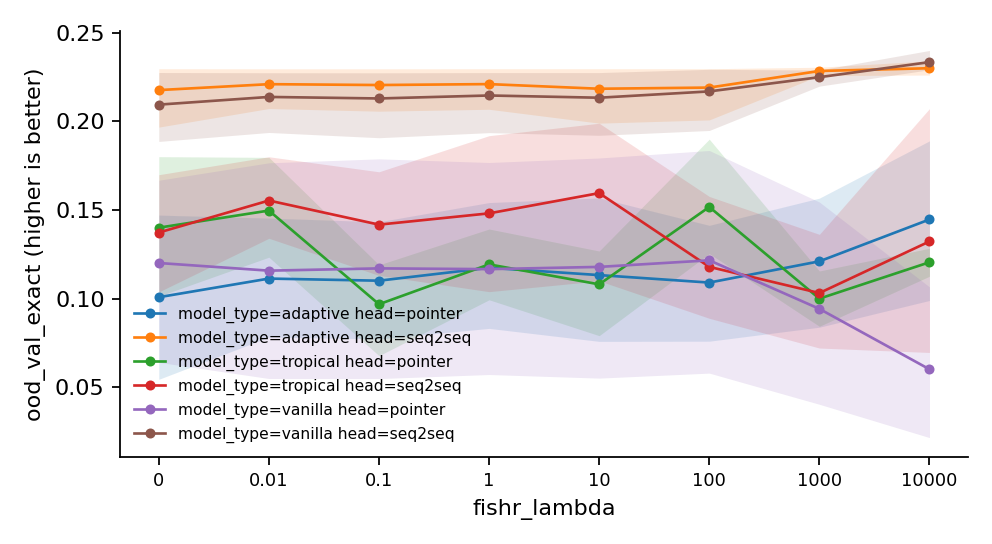
\includegraphics[width=\textwidth]{metric_ood_val_exact.png}
\caption{\texttt{ood\_val\_exact} against \texttt{fishr\_lambda}: the mean over seeds with a 95\% bootstrap CI, one line per combination of the other factors.}
\label{fig:ood_val_exact}
\end{figure}

{\small
\begin{longtable}{lllrlrrr}
\caption{\texttt{ood\_val\_exact} per cell: mean, 95\% bootstrap CI, SD, seeds, diverged runs.}\label{tab:summary-ood_val_exact}\\
\toprule
\texttt{model\_type} & \texttt{head} & \texttt{fishr\_lambda} & mean & 95\% CI & SD & $n$ & div.\\
\midrule
\endhead
adaptive & pointer & 0 & 0.1009 & [0.0546, 0.147] & 0.0609 & 5 & 0\\
adaptive & pointer & 0.01 & 0.1114 & [0.0784, 0.146] & 0.0441 & 5 & 0\\
adaptive & pointer & 0.1 & 0.1102 & [0.0774, 0.143] & 0.0433 & 5 & 0\\
adaptive & pointer & 1 & 0.1175 & [0.0833, 0.154] & 0.0456 & 5 & 0\\
adaptive & pointer & 10 & 0.1134 & [0.076, 0.157] & 0.0538 & 5 & 0\\
adaptive & pointer & 100 & 0.1091 & [0.0761, 0.141] & 0.041 & 5 & 0\\
adaptive & pointer & 1000 & 0.1211 & [0.084, 0.157] & 0.0477 & 5 & 0\\
adaptive & pointer & 1e+04 & 0.1447 & [0.099, 0.189] & 0.0601 & 5 & 0\\
adaptive & seq2seq & 0 & 0.2177 & [0.197, 0.23] & 0.0233 & 5 & 0\\
adaptive & seq2seq & 0.01 & 0.221 & [0.207, 0.23] & 0.0159 & 5 & 0\\
adaptive & seq2seq & 0.1 & 0.2206 & [0.206, 0.23] & 0.017 & 5 & 0\\
adaptive & seq2seq & 1 & 0.2211 & [0.207, 0.23] & 0.0159 & 5 & 0\\
adaptive & seq2seq & 10 & 0.2185 & [0.199, 0.23] & 0.0216 & 5 & 0\\
adaptive & seq2seq & 100 & 0.2191 & [0.201, 0.23] & 0.0204 & 5 & 0\\
adaptive & seq2seq & 1000 & 0.2285 & [0.226, 0.231] & 0.00303 & 5 & 0\\
adaptive & seq2seq & 1e+04 & 0.23 & [0.226, 0.234] & 0.0052 & 5 & 0\\
tropical & pointer & 0 & 0.1401 & [0.101, 0.18] & 0.049 & 5 & 0\\
tropical & pointer & 0.01 & 0.1498 & [0.123, 0.18] & 0.0355 & 5 & 0\\
tropical & pointer & 0.1 & 0.09692 & [0.0679, 0.119] & 0.0343 & 5 & 0\\
tropical & pointer & 1 & 0.1194 & [0.0994, 0.139] & 0.0256 & 5 & 0\\
tropical & pointer & 10 & 0.1081 & [0.0792, 0.127] & 0.0322 & 5 & 0\\
tropical & pointer & 100 & 0.1518 & [0.125, 0.19] & 0.0434 & 5 & 0\\
tropical & pointer & 1000 & 0.1001 & [0.0845, 0.116] & 0.0214 & 5 & 0\\
tropical & pointer & 1e+04 & 0.1206 & [0.113, 0.129] & 0.0106 & 5 & 0\\
tropical & seq2seq & 0 & 0.1374 & [0.104, 0.17] & 0.0426 & 5 & 0\\
tropical & seq2seq & 0.01 & 0.1554 & [0.134, 0.18] & 0.0298 & 5 & 0\\
tropical & seq2seq & 0.1 & 0.1418 & [0.113, 0.172] & 0.0346 & 5 & 0\\
tropical & seq2seq & 1 & 0.1482 & [0.104, 0.192] & 0.0573 & 5 & 0\\
tropical & seq2seq & 10 & 0.1596 & [0.11, 0.199] & 0.0579 & 5 & 0\\
tropical & seq2seq & 100 & 0.118 & [0.089, 0.158] & 0.0457 & 5 & 0\\
tropical & seq2seq & 1000 & 0.1032 & [0.0722, 0.136] & 0.0421 & 5 & 0\\
tropical & seq2seq & 1e+04 & 0.1323 & [0.0697, 0.207] & 0.0883 & 5 & 0\\
vanilla & pointer & 0 & 0.1202 & [0.0642, 0.167] & 0.0658 & 5 & 0\\
vanilla & pointer & 0.01 & 0.1159 & [0.055, 0.177] & 0.0798 & 5 & 0\\
vanilla & pointer & 0.1 & 0.1171 & [0.055, 0.179] & 0.0807 & 5 & 0\\
vanilla & pointer & 1 & 0.1167 & [0.0573, 0.177] & 0.0795 & 5 & 0\\
vanilla & pointer & 10 & 0.118 & [0.0553, 0.179] & 0.0807 & 5 & 0\\
vanilla & pointer & 100 & 0.1217 & [0.0581, 0.184] & 0.0822 & 5 & 0\\
vanilla & pointer & 1000 & 0.09432 & [0.0405, 0.155] & 0.0701 & 5 & 0\\
vanilla & pointer & 1e+04 & 0.06024 & [0.0217, 0.107] & 0.0534 & 5 & 0\\
vanilla & seq2seq & 0 & 0.2095 & [0.189, 0.228] & 0.0248 & 5 & 0\\
vanilla & seq2seq & 0.01 & 0.2138 & [0.194, 0.227] & 0.023 & 5 & 0\\
vanilla & seq2seq & 0.1 & 0.213 & [0.191, 0.227] & 0.0244 & 5 & 0\\
vanilla & seq2seq & 1 & 0.2147 & [0.194, 0.228] & 0.0233 & 5 & 0\\
vanilla & seq2seq & 10 & 0.2134 & [0.192, 0.228] & 0.0234 & 5 & 0\\
vanilla & seq2seq & 100 & 0.217 & [0.195, 0.229] & 0.0244 & 5 & 0\\
vanilla & seq2seq & 1000 & 0.225 & [0.22, 0.229] & 0.00628 & 5 & 0\\
vanilla & seq2seq & 1e+04 & 0.2335 & [0.229, 0.24] & 0.00746 & 5 & 0\\
\bottomrule
\end{longtable}
}

{\small
\begin{longtable}{lllrrrl}
\caption{\texttt{ood\_val\_exact}: each level of \texttt{fishr\_lambda} against its control (0), within each combination of the other factors. parametric: Dunnett vs control.}\label{tab:control-ood_val_exact}\\
\toprule
\texttt{model\_type} & \texttt{head} & \texttt{fishr\_lambda} & difference & 95\% CI & $p$ & \\
\midrule
\endhead
adaptive & pointer & 0.01 & 0.01052 & [-0.0769, 0.098] & 0.9996 & \\
adaptive & pointer & 0.1 & 0.00932 & [-0.0781, 0.0968] & 0.9998 & \\
adaptive & pointer & 1 & 0.01662 & [-0.0708, 0.104] & 0.9938 & \\
adaptive & pointer & 10 & 0.01248 & [-0.075, 0.0999] & 0.9989 & \\
adaptive & pointer & 100 & 0.00826 & [-0.0792, 0.0957] & 0.9999 & \\
adaptive & pointer & 1000 & 0.02024 & [-0.0672, 0.108] & 0.9815 & \\
adaptive & pointer & 1e+04 & 0.04386 & [-0.0436, 0.131] & 0.5982 & \\
adaptive & seq2seq & 0.01 & 0.00334 & [-0.026, 0.0327] & 0.9997 & \\
adaptive & seq2seq & 0.1 & 0.00286 & [-0.0265, 0.0322] & 0.9999 & \\
adaptive & seq2seq & 1 & 0.00338 & [-0.0259, 0.0327] & 0.9997 & \\
adaptive & seq2seq & 10 & $7.600\times10^{-4}$ & [-0.0286, 0.0301] & 1.0000 & \\
adaptive & seq2seq & 100 & 0.00142 & [-0.0279, 0.0307] & 1.0000 & \\
adaptive & seq2seq & 1000 & 0.01078 & [-0.0185, 0.0401] & 0.8456 & \\
adaptive & seq2seq & 1e+04 & 0.01234 & [-0.017, 0.0417] & 0.7541 & \\
tropical & pointer & 0.01 & 0.00966 & [-0.0489, 0.0682] & 0.9973 & \\
tropical & pointer & 0.1 & -0.04318 & [-0.102, 0.0153] & 0.2217 & \\
tropical & pointer & 1 & -0.0207 & [-0.0792, 0.0378] & 0.8669 & \\
tropical & pointer & 10 & -0.03196 & [-0.0905, 0.0266] & 0.5125 & \\
tropical & pointer & 100 & 0.0117 & [-0.0468, 0.0702] & 0.9917 & \\
tropical & pointer & 1000 & -0.04002 & [-0.0985, 0.0185] & 0.2879 & \\
tropical & pointer & 1e+04 & -0.0195 & [-0.078, 0.039] & 0.8953 & \\
tropical & seq2seq & 0.01 & 0.01806 & [-0.0739, 0.11] & 0.9926 & \\
tropical & seq2seq & 0.1 & 0.00446 & [-0.0875, 0.0965] & 1.0000 & \\
tropical & seq2seq & 1 & 0.01082 & [-0.0812, 0.103] & 0.9997 & \\
tropical & seq2seq & 10 & 0.02224 & [-0.0698, 0.114] & 0.9767 & \\
tropical & seq2seq & 100 & -0.01936 & [-0.111, 0.0726] & 0.9890 & \\
tropical & seq2seq & 1000 & -0.03412 & [-0.126, 0.0579] & 0.8408 & \\
tropical & seq2seq & 1e+04 & -0.00502 & [-0.097, 0.087] & 1.0000 & \\
vanilla & pointer & 0.01 & -0.00432 & [-0.135, 0.126] & 1.0000 & \\
vanilla & pointer & 0.1 & -0.00304 & [-0.133, 0.127] & 1.0000 & \\
vanilla & pointer & 1 & -0.00346 & [-0.134, 0.127] & 1.0000 & \\
vanilla & pointer & 10 & -0.0022 & [-0.133, 0.128] & 1.0000 & \\
vanilla & pointer & 100 & 0.00152 & [-0.129, 0.132] & 1.0000 & \\
vanilla & pointer & 1000 & -0.02586 & [-0.156, 0.105] & 0.9921 & \\
vanilla & pointer & 1e+04 & -0.05994 & [-0.19, 0.0705] & 0.6803 & \\
vanilla & seq2seq & 0.01 & 0.00434 & [-0.0323, 0.041] & 0.9997 & \\
vanilla & seq2seq & 0.1 & 0.00348 & [-0.0332, 0.0401] & 0.9999 & \\
vanilla & seq2seq & 1 & 0.00516 & [-0.0315, 0.0418] & 0.9990 & \\
vanilla & seq2seq & 10 & 0.0039 & [-0.0327, 0.0405] & 0.9998 & \\
vanilla & seq2seq & 100 & 0.00746 & [-0.0292, 0.0441] & 0.9908 & \\
vanilla & seq2seq & 1000 & 0.01548 & [-0.0212, 0.0521] & 0.7513 & \\
vanilla & seq2seq & 1e+04 & 0.02398 & [-0.0127, 0.0606] & 0.3293 & \\
\bottomrule
\end{longtable}
}

{\small
\begin{longtable}{llrrrrr}
\caption{\texttt{ood\_val\_exact} against log10 \texttt{fishr\_lambda}: parametric: OLS slope t-test, seed-bootstrap CI, with the Jonckheere--Terpstra ordered-trend $\tau$ and $p$.}\label{tab:trend-ood_val_exact}\\
\toprule
\texttt{model\_type} & \texttt{head} & estimate & 95\% CI & $p$ & JT $\tau$ & JT $p$\\
\midrule
\endhead
adaptive & pointer & 0.004054 & [$9.45\times10^{-4}$, 0.0071] & 0.2974 & 0.101 & 0.4543\\
adaptive & seq2seq & 0.00146 & [$7.14\times10^{-7}$, 0.00437] & 0.2502 & 0.158 & 0.2452\\
tropical & pointer & -0.001741 & [-0.00433, $5.10\times10^{-4}$] & 0.5614 & -0.0876 & 0.5251\\
tropical & seq2seq & -0.006306 & [-0.0167, 0.00478] & 0.1592 & -0.217 & 0.0980\\
vanilla & pointer & -0.007411 & [-0.0103, -0.00361] & 0.2278 & -0.145 & 0.2857\\
vanilla & seq2seq & 0.003044 & [$5.10\times10^{-4}$, 0.00627] & 0.0693 & 0.383 & 0.0032\\
\bottomrule
\end{longtable}
}

{\small
\begin{longtable}{lrrrl}
\caption{\texttt{ood\_val\_exact}: paired contrasts by seed, Holm-corrected across the cells. parametric: paired t-test by seed, Holm.}\label{tab:paired-ood_val_exact}\\
\toprule
contrast (within) & difference & 95\% CI & $p$ & \\
\midrule
\endhead
\stackcell{model\_type: tropical - vanilla\\\footnotesize head=pointer fishr\_lambda=0 } & 0.01992 & [-0.0532, 0.0931] & 1.0000 & \\
\stackcell{model\_type: tropical - vanilla\\\footnotesize head=pointer fishr\_lambda=0.01 } & 0.0339 & [-0.063, 0.131] & 1.0000 & \\
\stackcell{model\_type: tropical - vanilla\\\footnotesize head=pointer fishr\_lambda=0.1 } & -0.02022 & [-0.135, 0.095] & 1.0000 & \\
\stackcell{model\_type: tropical - vanilla\\\footnotesize head=pointer fishr\_lambda=1 } & 0.00268 & [-0.0942, 0.0995] & 1.0000 & \\
\stackcell{model\_type: tropical - vanilla\\\footnotesize head=pointer fishr\_lambda=10 } & -0.00984 & [-0.127, 0.107] & 1.0000 & \\
\stackcell{model\_type: tropical - vanilla\\\footnotesize head=pointer fishr\_lambda=100 } & 0.0301 & [-0.0611, 0.121] & 1.0000 & \\
\stackcell{model\_type: tropical - vanilla\\\footnotesize head=pointer fishr\_lambda=1000 } & 0.00576 & [-0.0796, 0.0911] & 1.0000 & \\
\stackcell{model\_type: tropical - vanilla\\\footnotesize head=pointer fishr\_lambda=1e+04 } & 0.06036 & [0.00246, 0.118] & 0.4881 & \\
\stackcell{model\_type: tropical - vanilla\\\footnotesize head=seq2seq fishr\_lambda=0 } & -0.07214 & [-0.132, -0.0122] & 0.3451 & \\
\stackcell{model\_type: tropical - vanilla\\\footnotesize head=seq2seq fishr\_lambda=0.01 } & -0.05842 & [-0.0984, -0.0184] & 0.2158 & \\
\stackcell{model\_type: tropical - vanilla\\\footnotesize head=seq2seq fishr\_lambda=0.1 } & -0.07116 & [-0.122, -0.0201] & 0.2338 & \\
\stackcell{model\_type: tropical - vanilla\\\footnotesize head=seq2seq fishr\_lambda=1 } & -0.06648 & [-0.144, 0.0112] & 0.6871 & \\
\stackcell{model\_type: tropical - vanilla\\\footnotesize head=seq2seq fishr\_lambda=10 } & -0.0538 & [-0.142, 0.0344] & 1.0000 & \\
\stackcell{model\_type: tropical - vanilla\\\footnotesize head=seq2seq fishr\_lambda=100 } & -0.09896 & [-0.157, -0.0406] & 0.1390 & \\
\stackcell{model\_type: tropical - vanilla\\\footnotesize head=seq2seq fishr\_lambda=1000 } & -0.1217 & [-0.176, -0.0678] & 0.0529 & \\
\stackcell{model\_type: tropical - vanilla\\\footnotesize head=seq2seq fishr\_lambda=1e+04 } & -0.1011 & [-0.213, 0.0108] & 0.6609 & \\
\stackcell{model\_type: adaptive - vanilla\\\footnotesize head=pointer fishr\_lambda=0 } & -0.0193 & [-0.11, 0.071] & 1.0000 & \\
\stackcell{model\_type: adaptive - vanilla\\\footnotesize head=pointer fishr\_lambda=0.01 } & -0.00446 & [-0.112, 0.103] & 1.0000 & \\
\stackcell{model\_type: adaptive - vanilla\\\footnotesize head=pointer fishr\_lambda=0.1 } & -0.00694 & [-0.116, 0.102] & 1.0000 & \\
\stackcell{model\_type: adaptive - vanilla\\\footnotesize head=pointer fishr\_lambda=1 } & $7.800\times10^{-4}$ & [-0.112, 0.114] & 1.0000 & \\
\stackcell{model\_type: adaptive - vanilla\\\footnotesize head=pointer fishr\_lambda=10 } & -0.00462 & [-0.123, 0.114] & 1.0000 & \\
\stackcell{model\_type: adaptive - vanilla\\\footnotesize head=pointer fishr\_lambda=100 } & -0.01256 & [-0.124, 0.099] & 1.0000 & \\
\stackcell{model\_type: adaptive - vanilla\\\footnotesize head=pointer fishr\_lambda=1000 } & 0.0268 & [-0.0953, 0.149] & 1.0000 & \\
\stackcell{model\_type: adaptive - vanilla\\\footnotesize head=pointer fishr\_lambda=1e+04 } & 0.0845 & [-0.0144, 0.183] & 1.0000 & \\
\stackcell{model\_type: adaptive - vanilla\\\footnotesize head=seq2seq fishr\_lambda=0 } & 0.0082 & [-0.0131, 0.0295] & 1.0000 & \\
\stackcell{model\_type: adaptive - vanilla\\\footnotesize head=seq2seq fishr\_lambda=0.01 } & 0.0072 & [-0.00497, 0.0194] & 1.0000 & \\
\stackcell{model\_type: adaptive - vanilla\\\footnotesize head=seq2seq fishr\_lambda=0.1 } & 0.00758 & [-0.00513, 0.0203] & 1.0000 & \\
\stackcell{model\_type: adaptive - vanilla\\\footnotesize head=seq2seq fishr\_lambda=1 } & 0.00642 & [-0.0048, 0.0176] & 1.0000 & \\
\stackcell{model\_type: adaptive - vanilla\\\footnotesize head=seq2seq fishr\_lambda=10 } & 0.00506 & [-0.00476, 0.0149] & 1.0000 & \\
\stackcell{model\_type: adaptive - vanilla\\\footnotesize head=seq2seq fishr\_lambda=100 } & 0.00216 & [-0.00295, 0.00727] & 1.0000 & \\
\stackcell{model\_type: adaptive - vanilla\\\footnotesize head=seq2seq fishr\_lambda=1000 } & 0.0035 & [-0.00502, 0.012] & 1.0000 & \\
\stackcell{model\_type: adaptive - vanilla\\\footnotesize head=seq2seq fishr\_lambda=1e+04 } & -0.00344 & [-0.0174, 0.0106] & 1.0000 & \\
\stackcell{head: pointer - seq2seq\\\footnotesize model\_type=adaptive fishr\_lambda=0 } & -0.1168 & [-0.178, -0.056] & 0.1190 & \\
\stackcell{head: pointer - seq2seq\\\footnotesize model\_type=adaptive fishr\_lambda=0.01 } & -0.1096 & [-0.161, -0.0586] & 0.0888 & \\
\stackcell{head: pointer - seq2seq\\\footnotesize model\_type=adaptive fishr\_lambda=0.1 } & -0.1104 & [-0.161, -0.0594] & 0.0888 & \\
\stackcell{head: pointer - seq2seq\\\footnotesize model\_type=adaptive fishr\_lambda=1 } & -0.1036 & [-0.158, -0.0489] & 0.1190 & \\
\stackcell{head: pointer - seq2seq\\\footnotesize model\_type=adaptive fishr\_lambda=10 } & -0.1051 & [-0.167, -0.0433] & 0.1557 & \\
\stackcell{head: pointer - seq2seq\\\footnotesize model\_type=adaptive fishr\_lambda=100 } & -0.11 & [-0.162, -0.0576] & 0.0903 & \\
\stackcell{head: pointer - seq2seq\\\footnotesize model\_type=adaptive fishr\_lambda=1000 } & -0.1074 & [-0.168, -0.0464] & 0.1455 & \\
\stackcell{head: pointer - seq2seq\\\footnotesize model\_type=adaptive fishr\_lambda=1e+04 } & -0.0853 & [-0.163, -0.00803] & 0.3510 & \\
\stackcell{head: pointer - seq2seq\\\footnotesize model\_type=tropical fishr\_lambda=0 } & 0.00274 & [-0.0659, 0.0713] & 1.0000 & \\
\stackcell{head: pointer - seq2seq\\\footnotesize model\_type=tropical fishr\_lambda=0.01 } & -0.00566 & [-0.0528, 0.0414] & 1.0000 & \\
\stackcell{head: pointer - seq2seq\\\footnotesize model\_type=tropical fishr\_lambda=0.1 } & -0.0449 & [-0.1, 0.0105] & 0.6126 & \\
\stackcell{head: pointer - seq2seq\\\footnotesize model\_type=tropical fishr\_lambda=1 } & -0.02878 & [-0.104, 0.0469] & 1.0000 & \\
\stackcell{head: pointer - seq2seq\\\footnotesize model\_type=tropical fishr\_lambda=10 } & -0.05146 & [-0.136, 0.0327] & 0.9894 & \\
\stackcell{head: pointer - seq2seq\\\footnotesize model\_type=tropical fishr\_lambda=100 } & 0.0338 & [0.00928, 0.0583] & 0.2614 & \\
\stackcell{head: pointer - seq2seq\\\footnotesize model\_type=tropical fishr\_lambda=1000 } & -0.00316 & [-0.0727, 0.0664] & 1.0000 & \\
\stackcell{head: pointer - seq2seq\\\footnotesize model\_type=tropical fishr\_lambda=1e+04 } & -0.01174 & [-0.116, 0.0923] & 1.0000 & \\
\stackcell{head: pointer - seq2seq\\\footnotesize model\_type=vanilla fishr\_lambda=0 } & -0.08932 & [-0.152, -0.0271] & 0.2448 & \\
\stackcell{head: pointer - seq2seq\\\footnotesize model\_type=vanilla fishr\_lambda=0.01 } & -0.09798 & [-0.18, -0.0162] & 0.3510 & \\
\stackcell{head: pointer - seq2seq\\\footnotesize model\_type=vanilla fishr\_lambda=0.1 } & -0.09584 & [-0.178, -0.0138] & 0.3510 & \\
\stackcell{head: pointer - seq2seq\\\footnotesize model\_type=vanilla fishr\_lambda=1 } & -0.09794 & [-0.178, -0.0184] & 0.3492 & \\
\stackcell{head: pointer - seq2seq\\\footnotesize model\_type=vanilla fishr\_lambda=10 } & -0.09542 & [-0.178, -0.0131] & 0.3510 & \\
\stackcell{head: pointer - seq2seq\\\footnotesize model\_type=vanilla fishr\_lambda=100 } & -0.09526 & [-0.176, -0.015] & 0.3510 & \\
\stackcell{head: pointer - seq2seq\\\footnotesize model\_type=vanilla fishr\_lambda=1000 } & -0.1307 & [-0.211, -0.0502] & 0.1718 & \\
\stackcell{head: pointer - seq2seq\\\footnotesize model\_type=vanilla fishr\_lambda=1e+04 } & -0.1732 & [-0.244, -0.103] & 0.0582 & \\
\bottomrule
\end{longtable}
}

\subsection{\texttt{ood\_noise\_f1}}
\begin{figure}[tbp]
\centering
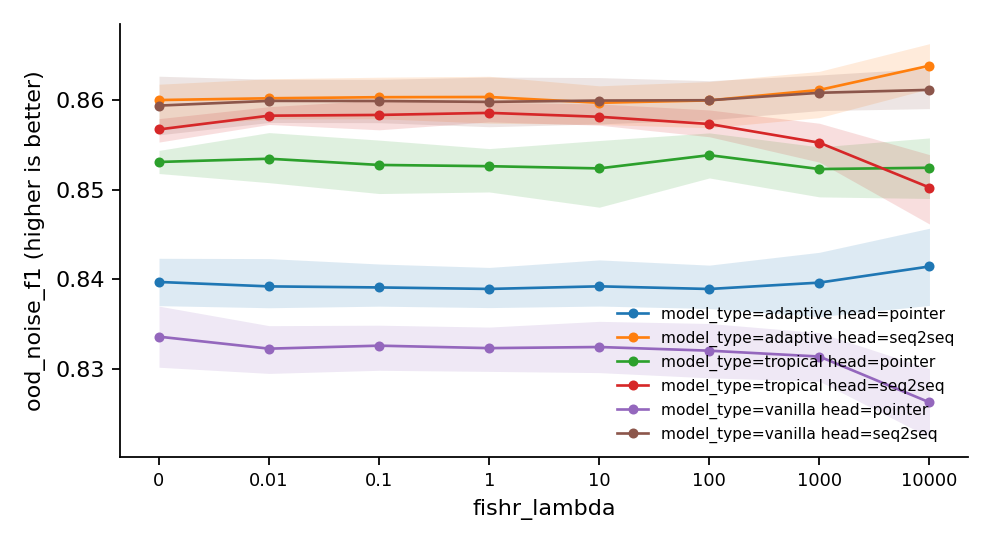
\includegraphics[width=\textwidth]{metric_ood_noise_f1.png}
\caption{\texttt{ood\_noise\_f1} against \texttt{fishr\_lambda}: the mean over seeds with a 95\% bootstrap CI, one line per combination of the other factors.}
\label{fig:ood_noise_f1}
\end{figure}

{\small
\begin{longtable}{lllrlrrr}
\caption{\texttt{ood\_noise\_f1} per cell: mean, 95\% bootstrap CI, SD, seeds, diverged runs.}\label{tab:summary-ood_noise_f1}\\
\toprule
\texttt{model\_type} & \texttt{head} & \texttt{fishr\_lambda} & mean & 95\% CI & SD & $n$ & div.\\
\midrule
\endhead
adaptive & pointer & 0 & 0.8397 & [0.837, 0.842] & 0.00351 & 5 & 0\\
adaptive & pointer & 0.01 & 0.8392 & [0.837, 0.842] & 0.00374 & 5 & 0\\
adaptive & pointer & 0.1 & 0.8391 & [0.837, 0.842] & 0.00301 & 5 & 0\\
adaptive & pointer & 1 & 0.8389 & [0.837, 0.841] & 0.00299 & 5 & 0\\
adaptive & pointer & 10 & 0.8392 & [0.837, 0.842] & 0.00332 & 5 & 0\\
adaptive & pointer & 100 & 0.8389 & [0.837, 0.842] & 0.00304 & 5 & 0\\
adaptive & pointer & 1000 & 0.8396 & [0.836, 0.843] & 0.00459 & 5 & 0\\
adaptive & pointer & 1e+04 & 0.8414 & [0.837, 0.846] & 0.00541 & 5 & 0\\
adaptive & seq2seq & 0 & 0.86 & [0.857, 0.862] & 0.00332 & 5 & 0\\
adaptive & seq2seq & 0.01 & 0.8602 & [0.858, 0.862] & 0.00304 & 5 & 0\\
adaptive & seq2seq & 0.1 & 0.8603 & [0.858, 0.863] & 0.00308 & 5 & 0\\
adaptive & seq2seq & 1 & 0.8603 & [0.857, 0.863] & 0.00322 & 5 & 0\\
adaptive & seq2seq & 10 & 0.8597 & [0.857, 0.862] & 0.00288 & 5 & 0\\
adaptive & seq2seq & 100 & 0.86 & [0.857, 0.862] & 0.00345 & 5 & 0\\
adaptive & seq2seq & 1000 & 0.8611 & [0.858, 0.863] & 0.0035 & 5 & 0\\
adaptive & seq2seq & 1e+04 & 0.8638 & [0.861, 0.866] & 0.00327 & 5 & 0\\
tropical & pointer & 0 & 0.8531 & [0.852, 0.854] & 0.00168 & 5 & 0\\
tropical & pointer & 0.01 & 0.8535 & [0.851, 0.856] & 0.00354 & 5 & 0\\
tropical & pointer & 0.1 & 0.8528 & [0.85, 0.856] & 0.00376 & 5 & 0\\
tropical & pointer & 1 & 0.8526 & [0.85, 0.855] & 0.00322 & 5 & 0\\
tropical & pointer & 10 & 0.8524 & [0.848, 0.855] & 0.00488 & 5 & 0\\
tropical & pointer & 100 & 0.8539 & [0.851, 0.856] & 0.00324 & 5 & 0\\
tropical & pointer & 1000 & 0.8523 & [0.849, 0.855] & 0.00394 & 5 & 0\\
tropical & pointer & 1e+04 & 0.8524 & [0.849, 0.856] & 0.00433 & 5 & 0\\
tropical & seq2seq & 0 & 0.8567 & [0.855, 0.858] & 0.0017 & 5 & 0\\
tropical & seq2seq & 0.01 & 0.8583 & [0.857, 0.859] & 0.00133 & 5 & 0\\
tropical & seq2seq & 0.1 & 0.8583 & [0.857, 0.86] & 0.00209 & 5 & 0\\
tropical & seq2seq & 1 & 0.8586 & [0.858, 0.86] & 0.00144 & 5 & 0\\
tropical & seq2seq & 10 & 0.8581 & [0.857, 0.86] & 0.00159 & 5 & 0\\
tropical & seq2seq & 100 & 0.8573 & [0.856, 0.859] & 0.00204 & 5 & 0\\
tropical & seq2seq & 1000 & 0.8552 & [0.853, 0.857] & 0.00293 & 5 & 0\\
tropical & seq2seq & 1e+04 & 0.8502 & [0.846, 0.854] & 0.00501 & 5 & 0\\
vanilla & pointer & 0 & 0.8336 & [0.83, 0.837] & 0.00436 & 5 & 0\\
vanilla & pointer & 0.01 & 0.8322 & [0.829, 0.835] & 0.0035 & 5 & 0\\
vanilla & pointer & 0.1 & 0.8326 & [0.83, 0.835] & 0.0032 & 5 & 0\\
vanilla & pointer & 1 & 0.8323 & [0.83, 0.835] & 0.00316 & 5 & 0\\
vanilla & pointer & 10 & 0.8324 & [0.83, 0.835] & 0.00369 & 5 & 0\\
vanilla & pointer & 100 & 0.832 & [0.829, 0.835] & 0.00386 & 5 & 0\\
vanilla & pointer & 1000 & 0.8314 & [0.829, 0.834] & 0.00361 & 5 & 0\\
vanilla & pointer & 1e+04 & 0.8263 & [0.822, 0.83] & 0.00523 & 5 & 0\\
vanilla & seq2seq & 0 & 0.8594 & [0.856, 0.863] & 0.00425 & 5 & 0\\
vanilla & seq2seq & 0.01 & 0.8599 & [0.858, 0.862] & 0.00314 & 5 & 0\\
vanilla & seq2seq & 0.1 & 0.8599 & [0.857, 0.862] & 0.00318 & 5 & 0\\
vanilla & seq2seq & 1 & 0.8598 & [0.857, 0.863] & 0.00365 & 5 & 0\\
vanilla & seq2seq & 10 & 0.8599 & [0.857, 0.863] & 0.00339 & 5 & 0\\
vanilla & seq2seq & 100 & 0.86 & [0.858, 0.862] & 0.00285 & 5 & 0\\
vanilla & seq2seq & 1000 & 0.8608 & [0.859, 0.863] & 0.00265 & 5 & 0\\
vanilla & seq2seq & 1e+04 & 0.8611 & [0.859, 0.864] & 0.00292 & 5 & 0\\
\bottomrule
\end{longtable}
}

{\small
\begin{longtable}{lllrrrl}
\caption{\texttt{ood\_noise\_f1}: each level of \texttt{fishr\_lambda} against its control (0), within each combination of the other factors. parametric: Dunnett vs control.}\label{tab:control-ood_noise_f1}\\
\toprule
\texttt{model\_type} & \texttt{head} & \texttt{fishr\_lambda} & difference & 95\% CI & $p$ & \\
\midrule
\endhead
adaptive & pointer & 0.01 & $-4.947\times10^{-4}$ & [-0.00712, 0.00613] & 1.0000 & \\
adaptive & pointer & 0.1 & $-6.112\times10^{-4}$ & [-0.00723, 0.00601] & 0.9999 & \\
adaptive & pointer & 1 & $-7.778\times10^{-4}$ & [-0.0074, 0.00584] & 0.9997 & \\
adaptive & pointer & 10 & $-4.867\times10^{-4}$ & [-0.00711, 0.00613] & 1.0000 & \\
adaptive & pointer & 100 & $-7.837\times10^{-4}$ & [-0.00741, 0.00584] & 0.9997 & \\
adaptive & pointer & 1000 & $-7.232\times10^{-5}$ & [-0.00669, 0.00655] & 1.0000 & \\
adaptive & pointer & 1e+04 & 0.001732 & [-0.00489, 0.00835] & 0.9652 & \\
adaptive & seq2seq & 0.01 & $1.970\times10^{-4}$ & [-0.00544, 0.00583] & 1.0000 & \\
adaptive & seq2seq & 0.1 & $3.185\times10^{-4}$ & [-0.00532, 0.00595] & 1.0000 & \\
adaptive & seq2seq & 1 & $3.422\times10^{-4}$ & [-0.00529, 0.00598] & 1.0000 & \\
adaptive & seq2seq & 10 & $-3.037\times10^{-4}$ & [-0.00594, 0.00533] & 1.0000 & \\
adaptive & seq2seq & 100 & $-3.890\times10^{-5}$ & [-0.00567, 0.0056] & 1.0000 & \\
adaptive & seq2seq & 1000 & 0.00113 & [-0.00451, 0.00677] & 0.9916 & \\
adaptive & seq2seq & 1e+04 & 0.003835 & [-0.0018, 0.00947] & 0.2924 & \\
tropical & pointer & 0.01 & $3.599\times10^{-4}$ & [-0.00607, 0.00679] & 1.0000 & \\
tropical & pointer & 0.1 & $-3.332\times10^{-4}$ & [-0.00676, 0.0061] & 1.0000 & \\
tropical & pointer & 1 & $-4.734\times10^{-4}$ & [-0.0069, 0.00596] & 1.0000 & \\
tropical & pointer & 10 & $-7.188\times10^{-4}$ & [-0.00715, 0.00571] & 0.9998 & \\
tropical & pointer & 100 & $7.601\times10^{-4}$ & [-0.00567, 0.00719] & 0.9997 & \\
tropical & pointer & 1000 & $-7.920\times10^{-4}$ & [-0.00722, 0.00564] & 0.9996 & \\
tropical & pointer & 1e+04 & $-6.456\times10^{-4}$ & [-0.00708, 0.00578] & 0.9999 & \\
tropical & seq2seq & 0.01 & 0.001534 & [-0.0029, 0.00597] & 0.8777 & \\
tropical & seq2seq & 0.1 & 0.001617 & [-0.00282, 0.00605] & 0.8506 & \\
tropical & seq2seq & 1 & 0.001847 & [-0.00259, 0.00628] & 0.7619 & \\
tropical & seq2seq & 10 & 0.001411 & [-0.00302, 0.00584] & 0.9135 & \\
tropical & seq2seq & 100 & $6.040\times10^{-4}$ & [-0.00383, 0.00504] & 0.9992 & \\
tropical & seq2seq & 1000 & -0.001485 & [-0.00592, 0.00295] & 0.8930 & \\
tropical & seq2seq & 1e+04 & -0.006489 & [-0.0109, -0.00206] & 0.0019 & *\\
vanilla & pointer & 0.01 & -0.001337 & [-0.00811, 0.00544] & 0.9923 & \\
vanilla & pointer & 0.1 & -0.001003 & [-0.00778, 0.00577] & 0.9986 & \\
vanilla & pointer & 1 & -0.001278 & [-0.00805, 0.0055] & 0.9941 & \\
vanilla & pointer & 10 & -0.001154 & [-0.00793, 0.00562] & 0.9968 & \\
vanilla & pointer & 100 & -0.001562 & [-0.00834, 0.00521] & 0.9819 & \\
vanilla & pointer & 1000 & -0.002217 & [-0.00899, 0.00456] & 0.9028 & \\
vanilla & pointer & 1e+04 & -0.007333 & [-0.0141, $-5.58\times10^{-4}$] & 0.0295 & *\\
vanilla & seq2seq & 0.01 & $5.279\times10^{-4}$ & [-0.00522, 0.00627] & 0.9999 & \\
vanilla & seq2seq & 0.1 & $5.147\times10^{-4}$ & [-0.00523, 0.00626] & 0.9999 & \\
vanilla & seq2seq & 1 & $4.149\times10^{-4}$ & [-0.00533, 0.00616] & 1.0000 & \\
vanilla & seq2seq & 10 & $5.644\times10^{-4}$ & [-0.00518, 0.00631] & 0.9999 & \\
vanilla & seq2seq & 100 & $5.986\times10^{-4}$ & [-0.00515, 0.00634] & 0.9999 & \\
vanilla & seq2seq & 1000 & 0.001431 & [-0.00431, 0.00718] & 0.9728 & \\
vanilla & seq2seq & 1e+04 & 0.001757 & [-0.00399, 0.0075] & 0.9274 & \\
\bottomrule
\end{longtable}
}

{\small
\begin{longtable}{llrrrrr}
\caption{\texttt{ood\_noise\_f1} against log10 \texttt{fishr\_lambda}: parametric: OLS slope t-test, seed-bootstrap CI, with the Jonckheere--Terpstra ordered-trend $\tau$ and $p$.}\label{tab:trend-ood_noise_f1}\\
\toprule
\texttt{model\_type} & \texttt{head} & estimate & 95\% CI & $p$ & JT $\tau$ & JT $p$\\
\midrule
\endhead
adaptive & pointer & $2.769\times10^{-4}$ & [$-2.79\times10^{-5}$, $4.91\times10^{-4}$] & 0.3672 & 0.0971 & 0.4699\\
adaptive & seq2seq & $4.342\times10^{-4}$ & [$2.62\times10^{-5}$, $7.88\times10^{-4}$] & 0.1101 & 0.2 & 0.1420\\
tropical & pointer & $-9.645\times10^{-5}$ & [$-5.91\times10^{-4}$, $3.84\times10^{-4}$] & 0.7543 & 0.00952 & 0.9464\\
tropical & seq2seq & -0.001126 & [-0.00156, $-7.70\times10^{-4}$] & $<10^{-4}$ & -0.478 & 0.0004\\
vanilla & pointer & $-7.393\times10^{-4}$ & [-0.00111, $-4.16\times10^{-4}$] & 0.0288 & -0.253 & 0.0564\\
vanilla & seq2seq & $2.037\times10^{-4}$ & [$-6.49\times10^{-5}$, $4.64\times10^{-4}$] & 0.4111 & 0.135 & 0.3069\\
\bottomrule
\end{longtable}
}

{\small
\begin{longtable}{lrrrl}
\caption{\texttt{ood\_noise\_f1}: paired contrasts by seed, Holm-corrected across the cells. parametric: paired t-test by seed, Holm.}\label{tab:paired-ood_noise_f1}\\
\toprule
contrast (within) & difference & 95\% CI & $p$ & \\
\midrule
\endhead
\stackcell{model\_type: tropical - vanilla\\\footnotesize head=pointer fishr\_lambda=0 } & 0.01951 & [0.0143, 0.0248] & 0.0079 & *\\
\stackcell{model\_type: tropical - vanilla\\\footnotesize head=pointer fishr\_lambda=0.01 } & 0.02121 & [0.0136, 0.0288] & 0.0194 & *\\
\stackcell{model\_type: tropical - vanilla\\\footnotesize head=pointer fishr\_lambda=0.1 } & 0.02018 & [0.0127, 0.0277] & 0.0209 & *\\
\stackcell{model\_type: tropical - vanilla\\\footnotesize head=pointer fishr\_lambda=1 } & 0.02031 & [0.0134, 0.0272] & 0.0183 & *\\
\stackcell{model\_type: tropical - vanilla\\\footnotesize head=pointer fishr\_lambda=10 } & 0.01994 & [0.0116, 0.0283] & 0.0272 & *\\
\stackcell{model\_type: tropical - vanilla\\\footnotesize head=pointer fishr\_lambda=100 } & 0.02183 & [0.0144, 0.0293] & 0.0183 & *\\
\stackcell{model\_type: tropical - vanilla\\\footnotesize head=pointer fishr\_lambda=1000 } & 0.02093 & [0.0124, 0.0295] & 0.0272 & *\\
\stackcell{model\_type: tropical - vanilla\\\footnotesize head=pointer fishr\_lambda=1e+04 } & 0.0262 & [0.0146, 0.0378] & 0.0301 & *\\
\stackcell{model\_type: tropical - vanilla\\\footnotesize head=seq2seq fishr\_lambda=0 } & -0.002659 & [-0.00778, 0.00246] & 1.0000 & \\
\stackcell{model\_type: tropical - vanilla\\\footnotesize head=seq2seq fishr\_lambda=0.01 } & -0.001652 & [-0.00575, 0.00245] & 1.0000 & \\
\stackcell{model\_type: tropical - vanilla\\\footnotesize head=seq2seq fishr\_lambda=0.1 } & -0.001557 & [-0.00619, 0.00308] & 1.0000 & \\
\stackcell{model\_type: tropical - vanilla\\\footnotesize head=seq2seq fishr\_lambda=1 } & -0.001227 & [-0.0058, 0.00335] & 1.0000 & \\
\stackcell{model\_type: tropical - vanilla\\\footnotesize head=seq2seq fishr\_lambda=10 } & -0.001812 & [-0.0054, 0.00178] & 1.0000 & \\
\stackcell{model\_type: tropical - vanilla\\\footnotesize head=seq2seq fishr\_lambda=100 } & -0.002654 & [-0.00666, 0.00135] & 0.8395 & \\
\stackcell{model\_type: tropical - vanilla\\\footnotesize head=seq2seq fishr\_lambda=1000 } & -0.005575 & [-0.0105, $-6.79\times10^{-4}$] & 0.2389 & \\
\stackcell{model\_type: tropical - vanilla\\\footnotesize head=seq2seq fishr\_lambda=1e+04 } & -0.0109 & [-0.0181, -0.00368] & 0.1105 & \\
\stackcell{model\_type: adaptive - vanilla\\\footnotesize head=pointer fishr\_lambda=0 } & 0.006109 & [-0.00339, 0.0156] & 1.0000 & \\
\stackcell{model\_type: adaptive - vanilla\\\footnotesize head=pointer fishr\_lambda=0.01 } & 0.006952 & [-0.00142, 0.0153] & 0.8836 & \\
\stackcell{model\_type: adaptive - vanilla\\\footnotesize head=pointer fishr\_lambda=0.1 } & 0.006501 & [$-3.61\times10^{-4}$, 0.0134] & 0.8463 & \\
\stackcell{model\_type: adaptive - vanilla\\\footnotesize head=pointer fishr\_lambda=1 } & 0.006609 & [$-2.91\times10^{-4}$, 0.0135] & 0.8463 & \\
\stackcell{model\_type: adaptive - vanilla\\\footnotesize head=pointer fishr\_lambda=10 } & 0.006776 & [-0.0013, 0.0149] & 0.8836 & \\
\stackcell{model\_type: adaptive - vanilla\\\footnotesize head=pointer fishr\_lambda=100 } & 0.006888 & [-0.00105, 0.0148] & 0.8836 & \\
\stackcell{model\_type: adaptive - vanilla\\\footnotesize head=pointer fishr\_lambda=1000 } & 0.008254 & [$-7.70\times10^{-4}$, 0.0173] & 0.8463 & \\
\stackcell{model\_type: adaptive - vanilla\\\footnotesize head=pointer fishr\_lambda=1e+04 } & 0.01517 & [0.0034, 0.0269] & 0.3710 & \\
\stackcell{model\_type: adaptive - vanilla\\\footnotesize head=seq2seq fishr\_lambda=0 } & $6.208\times10^{-4}$ & [-0.0037, 0.00495] & 1.0000 & \\
\stackcell{model\_type: adaptive - vanilla\\\footnotesize head=seq2seq fishr\_lambda=0.01 } & $2.899\times10^{-4}$ & [-0.00247, 0.00305] & 1.0000 & \\
\stackcell{model\_type: adaptive - vanilla\\\footnotesize head=seq2seq fishr\_lambda=0.1 } & $4.246\times10^{-4}$ & [-0.00261, 0.00346] & 1.0000 & \\
\stackcell{model\_type: adaptive - vanilla\\\footnotesize head=seq2seq fishr\_lambda=1 } & $5.482\times10^{-4}$ & [-0.00284, 0.00394] & 1.0000 & \\
\stackcell{model\_type: adaptive - vanilla\\\footnotesize head=seq2seq fishr\_lambda=10 } & $-2.473\times10^{-4}$ & [-0.00359, 0.0031] & 1.0000 & \\
\stackcell{model\_type: adaptive - vanilla\\\footnotesize head=seq2seq fishr\_lambda=100 } & $-1.670\times10^{-5}$ & [-0.00347, 0.00343] & 1.0000 & \\
\stackcell{model\_type: adaptive - vanilla\\\footnotesize head=seq2seq fishr\_lambda=1000 } & $3.200\times10^{-4}$ & [-0.00348, 0.00412] & 1.0000 & \\
\stackcell{model\_type: adaptive - vanilla\\\footnotesize head=seq2seq fishr\_lambda=1e+04 } & 0.0027 & [-0.00273, 0.00812] & 1.0000 & \\
\stackcell{head: pointer - seq2seq\\\footnotesize model\_type=adaptive fishr\_lambda=0 } & -0.02031 & [-0.0253, -0.0153] & 0.0076 & *\\
\stackcell{head: pointer - seq2seq\\\footnotesize model\_type=adaptive fishr\_lambda=0.01 } & -0.021 & [-0.0275, -0.0145] & 0.0105 & *\\
\stackcell{head: pointer - seq2seq\\\footnotesize model\_type=adaptive fishr\_lambda=0.1 } & -0.02124 & [-0.0274, -0.0151] & 0.0099 & *\\
\stackcell{head: pointer - seq2seq\\\footnotesize model\_type=adaptive fishr\_lambda=1 } & -0.02143 & [-0.0278, -0.015] & 0.0105 & *\\
\stackcell{head: pointer - seq2seq\\\footnotesize model\_type=adaptive fishr\_lambda=10 } & -0.0205 & [-0.0262, -0.0148] & 0.0091 & *\\
\stackcell{head: pointer - seq2seq\\\footnotesize model\_type=adaptive fishr\_lambda=100 } & -0.02106 & [-0.0274, -0.0147] & 0.0105 & *\\
\stackcell{head: pointer - seq2seq\\\footnotesize model\_type=adaptive fishr\_lambda=1000 } & -0.02152 & [-0.0295, -0.0136] & 0.0154 & *\\
\stackcell{head: pointer - seq2seq\\\footnotesize model\_type=adaptive fishr\_lambda=1e+04 } & -0.02242 & [-0.0305, -0.0143] & 0.0154 & *\\
\stackcell{head: pointer - seq2seq\\\footnotesize model\_type=tropical fishr\_lambda=0 } & -0.003634 & [-0.00678, $-4.84\times10^{-4}$] & 0.1987 & \\
\stackcell{head: pointer - seq2seq\\\footnotesize model\_type=tropical fishr\_lambda=0.01 } & -0.004808 & [-0.0105, $8.93\times10^{-4}$] & 0.3170 & \\
\stackcell{head: pointer - seq2seq\\\footnotesize model\_type=tropical fishr\_lambda=0.1 } & -0.005583 & [-0.0102, $-9.66\times10^{-4}$] & 0.1987 & \\
\stackcell{head: pointer - seq2seq\\\footnotesize model\_type=tropical fishr\_lambda=1 } & -0.005954 & [-0.0104, -0.0015] & 0.1654 & \\
\stackcell{head: pointer - seq2seq\\\footnotesize model\_type=tropical fishr\_lambda=10 } & -0.005764 & [-0.0111, $-3.93\times10^{-4}$] & 0.2037 & \\
\stackcell{head: pointer - seq2seq\\\footnotesize model\_type=tropical fishr\_lambda=100 } & -0.003477 & [-0.00789, $9.33\times10^{-4}$] & 0.3170 & \\
\stackcell{head: pointer - seq2seq\\\footnotesize model\_type=tropical fishr\_lambda=1000 } & -0.002941 & [-0.0098, 0.00392] & 0.5992 & \\
\stackcell{head: pointer - seq2seq\\\footnotesize model\_type=tropical fishr\_lambda=1e+04 } & 0.00221 & [-0.00822, 0.0126] & 0.5992 & \\
\stackcell{head: pointer - seq2seq\\\footnotesize model\_type=vanilla fishr\_lambda=0 } & -0.0258 & [-0.0343, -0.0173] & 0.0121 & *\\
\stackcell{head: pointer - seq2seq\\\footnotesize model\_type=vanilla fishr\_lambda=0.01 } & -0.02767 & [-0.0348, -0.0205] & 0.0086 & *\\
\stackcell{head: pointer - seq2seq\\\footnotesize model\_type=vanilla fishr\_lambda=0.1 } & -0.02732 & [-0.0343, -0.0203] & 0.0086 & *\\
\stackcell{head: pointer - seq2seq\\\footnotesize model\_type=vanilla fishr\_lambda=1 } & -0.02749 & [-0.0349, -0.0201] & 0.0089 & *\\
\stackcell{head: pointer - seq2seq\\\footnotesize model\_type=vanilla fishr\_lambda=10 } & -0.02752 & [-0.035, -0.0201] & 0.0089 & *\\
\stackcell{head: pointer - seq2seq\\\footnotesize model\_type=vanilla fishr\_lambda=100 } & -0.02796 & [-0.0352, -0.0207] & 0.0086 & *\\
\stackcell{head: pointer - seq2seq\\\footnotesize model\_type=vanilla fishr\_lambda=1000 } & -0.02945 & [-0.0364, -0.0225] & 0.0067 & *\\
\stackcell{head: pointer - seq2seq\\\footnotesize model\_type=vanilla fishr\_lambda=1e+04 } & -0.03489 & [-0.0419, -0.0279] & 0.0039 & *\\
\bottomrule
\end{longtable}
}

\subsection{\texttt{ood\_noise\_exact}}
\begin{figure}[tbp]
\centering
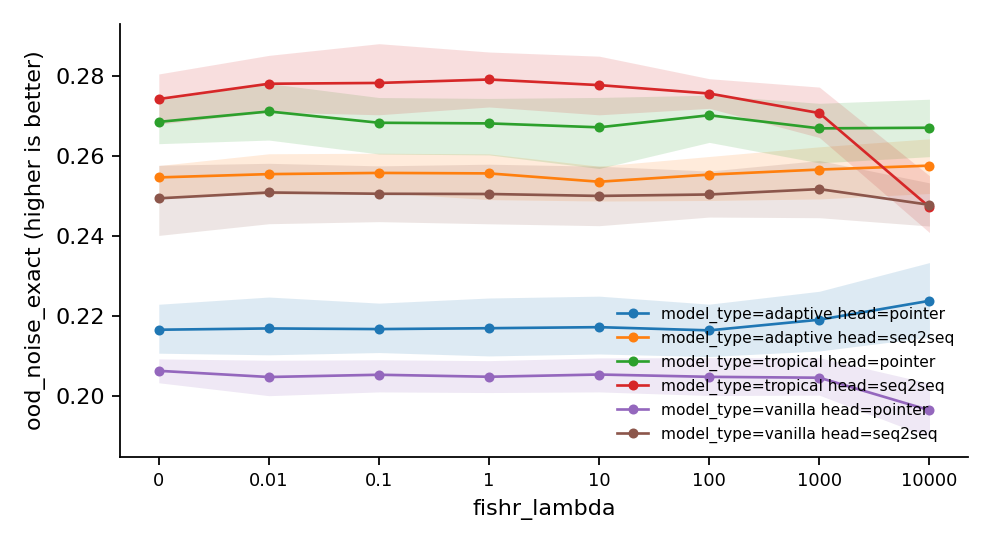
\includegraphics[width=\textwidth]{metric_ood_noise_exact.png}
\caption{\texttt{ood\_noise\_exact} against \texttt{fishr\_lambda}: the mean over seeds with a 95\% bootstrap CI, one line per combination of the other factors.}
\label{fig:ood_noise_exact}
\end{figure}

{\small
\begin{longtable}{lllrlrrr}
\caption{\texttt{ood\_noise\_exact} per cell: mean, 95\% bootstrap CI, SD, seeds, diverged runs.}\label{tab:summary-ood_noise_exact}\\
\toprule
\texttt{model\_type} & \texttt{head} & \texttt{fishr\_lambda} & mean & 95\% CI & SD & $n$ & div.\\
\midrule
\endhead
adaptive & pointer & 0 & 0.2166 & [0.211, 0.223] & 0.0077 & 5 & 0\\
adaptive & pointer & 0.01 & 0.217 & [0.21, 0.225] & 0.0094 & 5 & 0\\
adaptive & pointer & 0.1 & 0.2168 & [0.211, 0.223] & 0.00821 & 5 & 0\\
adaptive & pointer & 1 & 0.217 & [0.21, 0.225] & 0.00914 & 5 & 0\\
adaptive & pointer & 10 & 0.2173 & [0.211, 0.225] & 0.00949 & 5 & 0\\
adaptive & pointer & 100 & 0.2165 & [0.21, 0.223] & 0.00827 & 5 & 0\\
adaptive & pointer & 1000 & 0.2191 & [0.211, 0.226] & 0.00947 & 5 & 0\\
adaptive & pointer & 1e+04 & 0.2239 & [0.215, 0.233] & 0.0127 & 5 & 0\\
adaptive & seq2seq & 0 & 0.2547 & [0.25, 0.258] & 0.00511 & 5 & 0\\
adaptive & seq2seq & 0.01 & 0.2555 & [0.25, 0.261] & 0.00695 & 5 & 0\\
adaptive & seq2seq & 0.1 & 0.2558 & [0.251, 0.261] & 0.00656 & 5 & 0\\
adaptive & seq2seq & 1 & 0.2557 & [0.249, 0.261] & 0.00685 & 5 & 0\\
adaptive & seq2seq & 10 & 0.2536 & [0.249, 0.257] & 0.00583 & 5 & 0\\
adaptive & seq2seq & 100 & 0.2554 & [0.249, 0.26] & 0.00722 & 5 & 0\\
adaptive & seq2seq & 1000 & 0.2566 & [0.249, 0.262] & 0.00874 & 5 & 0\\
adaptive & seq2seq & 1e+04 & 0.2576 & [0.251, 0.264] & 0.00896 & 5 & 0\\
tropical & pointer & 0 & 0.2685 & [0.263, 0.274] & 0.007 & 5 & 0\\
tropical & pointer & 0.01 & 0.2711 & [0.264, 0.278] & 0.00916 & 5 & 0\\
tropical & pointer & 0.1 & 0.2683 & [0.261, 0.275] & 0.00941 & 5 & 0\\
tropical & pointer & 1 & 0.2681 & [0.26, 0.274] & 0.00942 & 5 & 0\\
tropical & pointer & 10 & 0.2672 & [0.257, 0.275] & 0.0116 & 5 & 0\\
tropical & pointer & 100 & 0.2702 & [0.263, 0.275] & 0.00783 & 5 & 0\\
tropical & pointer & 1000 & 0.2669 & [0.258, 0.273] & 0.0104 & 5 & 0\\
tropical & pointer & 1e+04 & 0.2671 & [0.26, 0.274] & 0.00943 & 5 & 0\\
tropical & seq2seq & 0 & 0.2742 & [0.268, 0.28] & 0.00836 & 5 & 0\\
tropical & seq2seq & 0.01 & 0.278 & [0.271, 0.285] & 0.00923 & 5 & 0\\
tropical & seq2seq & 0.1 & 0.2782 & [0.27, 0.288] & 0.0113 & 5 & 0\\
tropical & seq2seq & 1 & 0.2791 & [0.272, 0.286] & 0.00887 & 5 & 0\\
tropical & seq2seq & 10 & 0.2777 & [0.27, 0.285] & 0.00973 & 5 & 0\\
tropical & seq2seq & 100 & 0.2756 & [0.272, 0.279] & 0.00473 & 5 & 0\\
tropical & seq2seq & 1000 & 0.2707 & [0.265, 0.277] & 0.0081 & 5 & 0\\
tropical & seq2seq & 1e+04 & 0.2473 & [0.241, 0.255] & 0.00922 & 5 & 0\\
vanilla & pointer & 0 & 0.2064 & [0.203, 0.209] & 0.00383 & 5 & 0\\
vanilla & pointer & 0.01 & 0.2048 & [0.2, 0.209] & 0.00567 & 5 & 0\\
vanilla & pointer & 0.1 & 0.2054 & [0.201, 0.209] & 0.0054 & 5 & 0\\
vanilla & pointer & 1 & 0.2049 & [0.201, 0.209] & 0.00509 & 5 & 0\\
vanilla & pointer & 10 & 0.2055 & [0.201, 0.21] & 0.0054 & 5 & 0\\
vanilla & pointer & 100 & 0.2049 & [0.2, 0.21] & 0.00628 & 5 & 0\\
vanilla & pointer & 1000 & 0.2047 & [0.2, 0.21] & 0.00623 & 5 & 0\\
vanilla & pointer & 1e+04 & 0.1965 & [0.19, 0.203] & 0.00862 & 5 & 0\\
vanilla & seq2seq & 0 & 0.2494 & [0.24, 0.258] & 0.0111 & 5 & 0\\
vanilla & seq2seq & 0.01 & 0.2509 & [0.243, 0.258] & 0.00967 & 5 & 0\\
vanilla & seq2seq & 0.1 & 0.2506 & [0.244, 0.258] & 0.00937 & 5 & 0\\
vanilla & seq2seq & 1 & 0.2505 & [0.243, 0.258] & 0.0101 & 5 & 0\\
vanilla & seq2seq & 10 & 0.25 & [0.243, 0.257] & 0.00986 & 5 & 0\\
vanilla & seq2seq & 100 & 0.2504 & [0.245, 0.256] & 0.00747 & 5 & 0\\
vanilla & seq2seq & 1000 & 0.2517 & [0.245, 0.259] & 0.00947 & 5 & 0\\
vanilla & seq2seq & 1e+04 & 0.2478 & [0.243, 0.253] & 0.00683 & 5 & 0\\
\bottomrule
\end{longtable}
}

{\small
\begin{longtable}{lllrrrl}
\caption{\texttt{ood\_noise\_exact}: each level of \texttt{fishr\_lambda} against its control (0), within each combination of the other factors. parametric: Dunnett vs control.}\label{tab:control-ood_noise_exact}\\
\toprule
\texttt{model\_type} & \texttt{head} & \texttt{fishr\_lambda} & difference & 95\% CI & $p$ & \\
\midrule
\endhead
adaptive & pointer & 0.01 & $3.200\times10^{-4}$ & [-0.0161, 0.0167] & 1.0000 & \\
adaptive & pointer & 0.1 & $1.600\times10^{-4}$ & [-0.0163, 0.0166] & 1.0000 & \\
adaptive & pointer & 1 & $3.800\times10^{-4}$ & [-0.016, 0.0168] & 1.0000 & \\
adaptive & pointer & 10 & $6.400\times10^{-4}$ & [-0.0158, 0.0171] & 1.0000 & \\
adaptive & pointer & 100 & $-1.600\times10^{-4}$ & [-0.0166, 0.0163] & 1.0000 & \\
adaptive & pointer & 1000 & 0.0025 & [-0.0139, 0.0189] & 0.9984 & \\
adaptive & pointer & 1e+04 & 0.00722 & [-0.0092, 0.0236] & 0.7190 & \\
adaptive & seq2seq & 0.01 & $8.200\times10^{-4}$ & [-0.0116, 0.0133] & 1.0000 & \\
adaptive & seq2seq & 0.1 & 0.00112 & [-0.0113, 0.0136] & 0.9999 & \\
adaptive & seq2seq & 1 & 0.001 & [-0.0115, 0.0135] & 1.0000 & \\
adaptive & seq2seq & 10 & -0.00108 & [-0.0135, 0.0114] & 1.0000 & \\
adaptive & seq2seq & 100 & $7.000\times10^{-4}$ & [-0.0118, 0.0132] & 1.0000 & \\
adaptive & seq2seq & 1000 & 0.00196 & [-0.0105, 0.0144] & 0.9980 & \\
adaptive & seq2seq & 1e+04 & 0.00294 & [-0.00952, 0.0154] & 0.9795 & \\
tropical & pointer & 0.01 & 0.0026 & [-0.0138, 0.019] & 0.9979 & \\
tropical & pointer & 0.1 & $-2.200\times10^{-4}$ & [-0.0166, 0.0162] & 1.0000 & \\
tropical & pointer & 1 & $-3.800\times10^{-4}$ & [-0.0168, 0.016] & 1.0000 & \\
tropical & pointer & 10 & -0.00136 & [-0.0177, 0.015] & 1.0000 & \\
tropical & pointer & 100 & 0.00166 & [-0.0147, 0.018] & 0.9999 & \\
tropical & pointer & 1000 & -0.00162 & [-0.018, 0.0148] & 0.9999 & \\
tropical & pointer & 1e+04 & -0.00146 & [-0.0178, 0.0149] & 0.9999 & \\
tropical & seq2seq & 0.01 & 0.00382 & [-0.0117, 0.0193] & 0.9742 & \\
tropical & seq2seq & 0.1 & 0.00402 & [-0.0115, 0.0195] & 0.9666 & \\
tropical & seq2seq & 1 & 0.00488 & [-0.0106, 0.0204] & 0.9173 & \\
tropical & seq2seq & 10 & 0.00348 & [-0.012, 0.019] & 0.9842 & \\
tropical & seq2seq & 100 & 0.00138 & [-0.0141, 0.0169] & 0.9999 & \\
tropical & seq2seq & 1000 & -0.0035 & [-0.019, 0.012] & 0.9837 & \\
tropical & seq2seq & 1e+04 & -0.02696 & [-0.0424, -0.0115] & 0.0002 & *\\
vanilla & pointer & 0.01 & -0.00154 & [-0.0119, 0.00886] & 0.9986 & \\
vanilla & pointer & 0.1 & $-9.800\times10^{-4}$ & [-0.0114, 0.00942] & 0.9999 & \\
vanilla & pointer & 1 & -0.00148 & [-0.0119, 0.00892] & 0.9989 & \\
vanilla & pointer & 10 & $-9.200\times10^{-4}$ & [-0.0113, 0.00948] & 1.0000 & \\
vanilla & pointer & 100 & -0.0015 & [-0.0119, 0.0089] & 0.9988 & \\
vanilla & pointer & 1000 & -0.00172 & [-0.0121, 0.00868] & 0.9973 & \\
vanilla & pointer & 1e+04 & -0.00984 & [-0.0202, $5.60\times10^{-4}$] & 0.0698 & \\
vanilla & seq2seq & 0.01 & 0.00146 & [-0.0148, 0.0177] & 0.9999 & \\
vanilla & seq2seq & 0.1 & 0.00114 & [-0.0151, 0.0174] & 1.0000 & \\
vanilla & seq2seq & 1 & 0.00108 & [-0.0152, 0.0174] & 1.0000 & \\
vanilla & seq2seq & 10 & $6.000\times10^{-4}$ & [-0.0157, 0.0169] & 1.0000 & \\
vanilla & seq2seq & 100 & $9.600\times10^{-4}$ & [-0.0153, 0.0172] & 1.0000 & \\
vanilla & seq2seq & 1000 & 0.0023 & [-0.014, 0.0186] & 0.9990 & \\
vanilla & seq2seq & 1e+04 & -0.00162 & [-0.0179, 0.0147] & 0.9999 & \\
\bottomrule
\end{longtable}
}

{\small
\begin{longtable}{llrrrrr}
\caption{\texttt{ood\_noise\_exact} against log10 \texttt{fishr\_lambda}: parametric: OLS slope t-test, seed-bootstrap CI, with the Jonckheere--Terpstra ordered-trend $\tau$ and $p$.}\label{tab:trend-ood_noise_exact}\\
\toprule
\texttt{model\_type} & \texttt{head} & estimate & 95\% CI & $p$ & JT $\tau$ & JT $p$\\
\midrule
\endhead
adaptive & pointer & $8.871\times10^{-4}$ & [$4.91\times10^{-4}$, 0.00128] & 0.2532 & 0.137 & 0.3001\\
adaptive & seq2seq & $2.764\times10^{-4}$ & [$-5.94\times10^{-4}$, 0.00111] & 0.6373 & 0.0781 & 0.5645\\
tropical & pointer & $-4.621\times10^{-4}$ & [-0.00152, $6.53\times10^{-4}$] & 0.5474 & -0.0667 & 0.6251\\
tropical & seq2seq & -0.00396 & [-0.00426, -0.00367] & 0.0002 & -0.404 & 0.0024\\
vanilla & pointer & $-9.429\times10^{-4}$ & [-0.00145, $-4.46\times10^{-4}$] & 0.0804 & -0.179 & 0.1814\\
vanilla & seq2seq & $-2.514\times10^{-4}$ & [$-8.14\times10^{-4}$, $3.11\times10^{-4}$] & 0.7251 & -0.0514 & 0.6983\\
\bottomrule
\end{longtable}
}

{\small
\begin{longtable}{lrrrl}
\caption{\texttt{ood\_noise\_exact}: paired contrasts by seed, Holm-corrected across the cells. parametric: paired t-test by seed, Holm.}\label{tab:paired-ood_noise_exact}\\
\toprule
contrast (within) & difference & 95\% CI & $p$ & \\
\midrule
\endhead
\stackcell{model\_type: tropical - vanilla\\\footnotesize head=pointer fishr\_lambda=0 } & 0.06214 & [0.0518, 0.0725] & 0.0012 & *\\
\stackcell{model\_type: tropical - vanilla\\\footnotesize head=pointer fishr\_lambda=0.01 } & 0.06628 & [0.0514, 0.0812] & 0.0032 & *\\
\stackcell{model\_type: tropical - vanilla\\\footnotesize head=pointer fishr\_lambda=0.1 } & 0.0629 & [0.0466, 0.0792] & 0.0052 & *\\
\stackcell{model\_type: tropical - vanilla\\\footnotesize head=pointer fishr\_lambda=1 } & 0.06324 & [0.0495, 0.077] & 0.0031 & *\\
\stackcell{model\_type: tropical - vanilla\\\footnotesize head=pointer fishr\_lambda=10 } & 0.0617 & [0.045, 0.0784] & 0.0056 & *\\
\stackcell{model\_type: tropical - vanilla\\\footnotesize head=pointer fishr\_lambda=100 } & 0.0653 & [0.0515, 0.0791] & 0.0029 & *\\
\stackcell{model\_type: tropical - vanilla\\\footnotesize head=pointer fishr\_lambda=1000 } & 0.06224 & [0.0445, 0.08] & 0.0062 & *\\
\stackcell{model\_type: tropical - vanilla\\\footnotesize head=pointer fishr\_lambda=1e+04 } & 0.07052 & [0.0484, 0.0927] & 0.0081 & *\\
\stackcell{model\_type: tropical - vanilla\\\footnotesize head=seq2seq fishr\_lambda=0 } & 0.02478 & [0.00521, 0.0444] & 0.0550 & \\
\stackcell{model\_type: tropical - vanilla\\\footnotesize head=seq2seq fishr\_lambda=0.01 } & 0.02714 & [0.0111, 0.0432] & 0.0470 & *\\
\stackcell{model\_type: tropical - vanilla\\\footnotesize head=seq2seq fishr\_lambda=0.1 } & 0.02766 & [0.00935, 0.046] & 0.0550 & \\
\stackcell{model\_type: tropical - vanilla\\\footnotesize head=seq2seq fishr\_lambda=1 } & 0.02858 & [0.0128, 0.0444] & 0.0442 & *\\
\stackcell{model\_type: tropical - vanilla\\\footnotesize head=seq2seq fishr\_lambda=10 } & 0.02766 & [0.0142, 0.0411] & 0.0329 & *\\
\stackcell{model\_type: tropical - vanilla\\\footnotesize head=seq2seq fishr\_lambda=100 } & 0.0252 & [0.0145, 0.0359] & 0.0228 & *\\
\stackcell{model\_type: tropical - vanilla\\\footnotesize head=seq2seq fishr\_lambda=1000 } & 0.01898 & [0.00596, 0.032] & 0.0550 & \\
\stackcell{model\_type: tropical - vanilla\\\footnotesize head=seq2seq fishr\_lambda=1e+04 } & $-5.600\times10^{-4}$ & [-0.0116, 0.0105] & 0.8946 & \\
\stackcell{model\_type: adaptive - vanilla\\\footnotesize head=pointer fishr\_lambda=0 } & 0.01026 & [-0.00367, 0.0242] & 1.0000 & \\
\stackcell{model\_type: adaptive - vanilla\\\footnotesize head=pointer fishr\_lambda=0.01 } & 0.01212 & [-0.0038, 0.028] & 1.0000 & \\
\stackcell{model\_type: adaptive - vanilla\\\footnotesize head=pointer fishr\_lambda=0.1 } & 0.0114 & [-0.00132, 0.0241] & 0.9471 & \\
\stackcell{model\_type: adaptive - vanilla\\\footnotesize head=pointer fishr\_lambda=1 } & 0.01212 & [-0.00252, 0.0268] & 1.0000 & \\
\stackcell{model\_type: adaptive - vanilla\\\footnotesize head=pointer fishr\_lambda=10 } & 0.01182 & [-0.00425, 0.0279] & 1.0000 & \\
\stackcell{model\_type: adaptive - vanilla\\\footnotesize head=pointer fishr\_lambda=100 } & 0.0116 & [-0.00331, 0.0265] & 1.0000 & \\
\stackcell{model\_type: adaptive - vanilla\\\footnotesize head=pointer fishr\_lambda=1000 } & 0.01448 & [$-1.94\times10^{-4}$, 0.0292] & 0.7788 & \\
\stackcell{model\_type: adaptive - vanilla\\\footnotesize head=pointer fishr\_lambda=1e+04 } & 0.02732 & [0.00563, 0.049] & 0.3996 & \\
\stackcell{model\_type: adaptive - vanilla\\\footnotesize head=seq2seq fishr\_lambda=0 } & 0.00522 & [-0.00679, 0.0172] & 1.0000 & \\
\stackcell{model\_type: adaptive - vanilla\\\footnotesize head=seq2seq fishr\_lambda=0.01 } & 0.00458 & [-0.00261, 0.0118] & 1.0000 & \\
\stackcell{model\_type: adaptive - vanilla\\\footnotesize head=seq2seq fishr\_lambda=0.1 } & 0.0052 & [-0.00319, 0.0136] & 1.0000 & \\
\stackcell{model\_type: adaptive - vanilla\\\footnotesize head=seq2seq fishr\_lambda=1 } & 0.00514 & [-0.00325, 0.0135] & 1.0000 & \\
\stackcell{model\_type: adaptive - vanilla\\\footnotesize head=seq2seq fishr\_lambda=10 } & 0.00354 & [-0.00553, 0.0126] & 1.0000 & \\
\stackcell{model\_type: adaptive - vanilla\\\footnotesize head=seq2seq fishr\_lambda=100 } & 0.00496 & [-0.00261, 0.0125] & 1.0000 & \\
\stackcell{model\_type: adaptive - vanilla\\\footnotesize head=seq2seq fishr\_lambda=1000 } & 0.00488 & [-0.00244, 0.0122] & 1.0000 & \\
\stackcell{model\_type: adaptive - vanilla\\\footnotesize head=seq2seq fishr\_lambda=1e+04 } & 0.00978 & [-0.00283, 0.0224] & 1.0000 & \\
\stackcell{head: pointer - seq2seq\\\footnotesize model\_type=adaptive fishr\_lambda=0 } & -0.03802 & [-0.05, -0.026] & 0.0219 & *\\
\stackcell{head: pointer - seq2seq\\\footnotesize model\_type=adaptive fishr\_lambda=0.01 } & -0.03852 & [-0.0556, -0.0215] & 0.0397 & *\\
\stackcell{head: pointer - seq2seq\\\footnotesize model\_type=adaptive fishr\_lambda=0.1 } & -0.03898 & [-0.0552, -0.0228] & 0.0393 & *\\
\stackcell{head: pointer - seq2seq\\\footnotesize model\_type=adaptive fishr\_lambda=1 } & -0.03864 & [-0.0557, -0.0216] & 0.0397 & *\\
\stackcell{head: pointer - seq2seq\\\footnotesize model\_type=adaptive fishr\_lambda=10 } & -0.0363 & [-0.052, -0.0206] & 0.0397 & *\\
\stackcell{head: pointer - seq2seq\\\footnotesize model\_type=adaptive fishr\_lambda=100 } & -0.03888 & [-0.0553, -0.0225] & 0.0393 & *\\
\stackcell{head: pointer - seq2seq\\\footnotesize model\_type=adaptive fishr\_lambda=1000 } & -0.03748 & [-0.0567, -0.0183] & 0.0563 & \\
\stackcell{head: pointer - seq2seq\\\footnotesize model\_type=adaptive fishr\_lambda=1e+04 } & -0.03374 & [-0.0546, -0.0129] & 0.0983 & \\
\stackcell{head: pointer - seq2seq\\\footnotesize model\_type=tropical fishr\_lambda=0 } & -0.0057 & [-0.0145, 0.00309] & 0.7306 & \\
\stackcell{head: pointer - seq2seq\\\footnotesize model\_type=tropical fishr\_lambda=0.01 } & -0.00692 & [-0.0244, 0.0106] & 0.7306 & \\
\stackcell{head: pointer - seq2seq\\\footnotesize model\_type=tropical fishr\_lambda=0.1 } & -0.00994 & [-0.0263, 0.00643] & 0.7306 & \\
\stackcell{head: pointer - seq2seq\\\footnotesize model\_type=tropical fishr\_lambda=1 } & -0.01096 & [-0.0207, -0.00123] & 0.2469 & \\
\stackcell{head: pointer - seq2seq\\\footnotesize model\_type=tropical fishr\_lambda=10 } & -0.01054 & [-0.0187, -0.00235] & 0.1868 & \\
\stackcell{head: pointer - seq2seq\\\footnotesize model\_type=tropical fishr\_lambda=100 } & -0.00542 & [-0.0151, 0.00421] & 0.7306 & \\
\stackcell{head: pointer - seq2seq\\\footnotesize model\_type=tropical fishr\_lambda=1000 } & -0.00382 & [-0.0161, 0.00843] & 0.7306 & \\
\stackcell{head: pointer - seq2seq\\\footnotesize model\_type=tropical fishr\_lambda=1e+04 } & 0.0198 & [0.0015, 0.0381] & 0.2469 & \\
\stackcell{head: pointer - seq2seq\\\footnotesize model\_type=vanilla fishr\_lambda=0 } & -0.04306 & [-0.0595, -0.0266] & 0.0304 & *\\
\stackcell{head: pointer - seq2seq\\\footnotesize model\_type=vanilla fishr\_lambda=0.01 } & -0.04606 & [-0.0628, -0.0293] & 0.0301 & *\\
\stackcell{head: pointer - seq2seq\\\footnotesize model\_type=vanilla fishr\_lambda=0.1 } & -0.04518 & [-0.0619, -0.0285] & 0.0301 & *\\
\stackcell{head: pointer - seq2seq\\\footnotesize model\_type=vanilla fishr\_lambda=1 } & -0.04562 & [-0.0619, -0.0293] & 0.0298 & *\\
\stackcell{head: pointer - seq2seq\\\footnotesize model\_type=vanilla fishr\_lambda=10 } & -0.04458 & [-0.0601, -0.0291] & 0.0282 & *\\
\stackcell{head: pointer - seq2seq\\\footnotesize model\_type=vanilla fishr\_lambda=100 } & -0.04552 & [-0.0599, -0.0312] & 0.0219 & *\\
\stackcell{head: pointer - seq2seq\\\footnotesize model\_type=vanilla fishr\_lambda=1000 } & -0.04708 & [-0.0643, -0.0298] & 0.0301 & *\\
\stackcell{head: pointer - seq2seq\\\footnotesize model\_type=vanilla fishr\_lambda=1e+04 } & -0.05128 & [-0.0676, -0.035] & 0.0219 & *\\
\bottomrule
\end{longtable}
}

\subsection{\texttt{id\_f1}}
\begin{figure}[tbp]
\centering
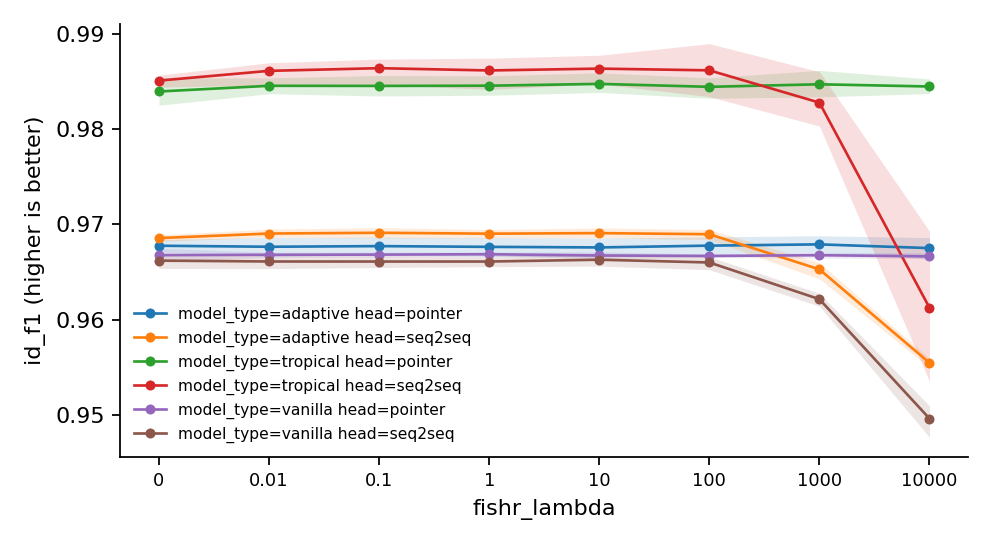
\includegraphics[width=\textwidth]{metric_id_f1.png}
\caption{\texttt{id\_f1} against \texttt{fishr\_lambda}: the mean over seeds with a 95\% bootstrap CI, one line per combination of the other factors.}
\label{fig:id_f1}
\end{figure}

{\small
\begin{longtable}{lllrlrrr}
\caption{\texttt{id\_f1} per cell: mean, 95\% bootstrap CI, SD, seeds, diverged runs.}\label{tab:summary-id_f1}\\
\toprule
\texttt{model\_type} & \texttt{head} & \texttt{fishr\_lambda} & mean & 95\% CI & SD & $n$ & div.\\
\midrule
\endhead
adaptive & pointer & 0 & 0.9677 & [0.967, 0.968] & $8.79\times10^{-4}$ & 5 & 0\\
adaptive & pointer & 0.01 & 0.9676 & [0.967, 0.969] & 0.00126 & 5 & 0\\
adaptive & pointer & 0.1 & 0.9677 & [0.967, 0.969] & 0.00124 & 5 & 0\\
adaptive & pointer & 1 & 0.9676 & [0.967, 0.969] & 0.00126 & 5 & 0\\
adaptive & pointer & 10 & 0.9676 & [0.967, 0.969] & 0.00131 & 5 & 0\\
adaptive & pointer & 100 & 0.9678 & [0.967, 0.969] & 0.00121 & 5 & 0\\
adaptive & pointer & 1000 & 0.9679 & [0.967, 0.969] & 0.00118 & 5 & 0\\
adaptive & pointer & 1e+04 & 0.9675 & [0.966, 0.969] & 0.00138 & 5 & 0\\
adaptive & seq2seq & 0 & 0.9686 & [0.968, 0.969] & $4.46\times10^{-4}$ & 5 & 0\\
adaptive & seq2seq & 0.01 & 0.969 & [0.969, 0.969] & $5.22\times10^{-4}$ & 5 & 0\\
adaptive & seq2seq & 0.1 & 0.9691 & [0.969, 0.97] & $6.92\times10^{-4}$ & 5 & 0\\
adaptive & seq2seq & 1 & 0.969 & [0.969, 0.969] & $5.93\times10^{-4}$ & 5 & 0\\
adaptive & seq2seq & 10 & 0.9691 & [0.969, 0.97] & $6.42\times10^{-4}$ & 5 & 0\\
adaptive & seq2seq & 100 & 0.969 & [0.968, 0.969] & $6.36\times10^{-4}$ & 5 & 0\\
adaptive & seq2seq & 1000 & 0.9653 & [0.964, 0.966] & 0.00108 & 5 & 0\\
adaptive & seq2seq & 1e+04 & 0.9555 & [0.955, 0.956] & $6.37\times10^{-4}$ & 5 & 0\\
tropical & pointer & 0 & 0.9839 & [0.982, 0.985] & 0.0019 & 5 & 0\\
tropical & pointer & 0.01 & 0.9845 & [0.984, 0.985] & 0.00107 & 5 & 0\\
tropical & pointer & 0.1 & 0.9845 & [0.983, 0.986] & 0.00141 & 5 & 0\\
tropical & pointer & 1 & 0.9845 & [0.984, 0.986] & 0.00131 & 5 & 0\\
tropical & pointer & 10 & 0.9847 & [0.984, 0.986] & 0.00133 & 5 & 0\\
tropical & pointer & 100 & 0.9844 & [0.983, 0.985] & 0.00132 & 5 & 0\\
tropical & pointer & 1000 & 0.9847 & [0.983, 0.986] & 0.00181 & 5 & 0\\
tropical & pointer & 1e+04 & 0.9844 & [0.984, 0.985] & 0.00101 & 5 & 0\\
tropical & seq2seq & 0 & 0.9851 & [0.984, 0.986] & $7.99\times10^{-4}$ & 5 & 0\\
tropical & seq2seq & 0.01 & 0.9861 & [0.985, 0.987] & 0.00166 & 5 & 0\\
tropical & seq2seq & 0.1 & 0.9864 & [0.985, 0.987] & 0.00193 & 5 & 0\\
tropical & seq2seq & 1 & 0.9861 & [0.984, 0.987] & 0.00218 & 5 & 0\\
tropical & seq2seq & 10 & 0.9863 & [0.985, 0.988] & 0.00195 & 5 & 0\\
tropical & seq2seq & 100 & 0.9861 & [0.983, 0.989] & 0.00346 & 5 & 0\\
tropical & seq2seq & 1000 & 0.9828 & [0.98, 0.986] & 0.00367 & 5 & 0\\
tropical & seq2seq & 1e+04 & 0.9612 & [0.954, 0.969] & 0.0105 & 5 & 0\\
vanilla & pointer & 0 & 0.9668 & [0.966, 0.967] & $9.30\times10^{-4}$ & 5 & 0\\
vanilla & pointer & 0.01 & 0.9668 & [0.967, 0.967] & $3.28\times10^{-4}$ & 5 & 0\\
vanilla & pointer & 0.1 & 0.9668 & [0.967, 0.967] & $3.22\times10^{-4}$ & 5 & 0\\
vanilla & pointer & 1 & 0.9669 & [0.967, 0.967] & $2.74\times10^{-4}$ & 5 & 0\\
vanilla & pointer & 10 & 0.9667 & [0.966, 0.967] & $4.80\times10^{-4}$ & 5 & 0\\
vanilla & pointer & 100 & 0.9667 & [0.967, 0.967] & $2.41\times10^{-4}$ & 5 & 0\\
vanilla & pointer & 1000 & 0.9668 & [0.966, 0.967] & $3.78\times10^{-4}$ & 5 & 0\\
vanilla & pointer & 1e+04 & 0.9666 & [0.966, 0.967] & $4.26\times10^{-4}$ & 5 & 0\\
vanilla & seq2seq & 0 & 0.9662 & [0.965, 0.967] & 0.00103 & 5 & 0\\
vanilla & seq2seq & 0.01 & 0.9661 & [0.965, 0.967] & $8.43\times10^{-4}$ & 5 & 0\\
vanilla & seq2seq & 0.1 & 0.9661 & [0.965, 0.967] & $8.03\times10^{-4}$ & 5 & 0\\
vanilla & seq2seq & 1 & 0.9661 & [0.966, 0.967] & $7.14\times10^{-4}$ & 5 & 0\\
vanilla & seq2seq & 10 & 0.9663 & [0.966, 0.967] & $8.70\times10^{-4}$ & 5 & 0\\
vanilla & seq2seq & 100 & 0.966 & [0.965, 0.967] & $8.59\times10^{-4}$ & 5 & 0\\
vanilla & seq2seq & 1000 & 0.9621 & [0.961, 0.963] & $8.63\times10^{-4}$ & 5 & 0\\
vanilla & seq2seq & 1e+04 & 0.9496 & [0.948, 0.951] & 0.0022 & 5 & 0\\
\bottomrule
\end{longtable}
}

{\small
\begin{longtable}{lllrrrl}
\caption{\texttt{id\_f1}: each level of \texttt{fishr\_lambda} against its control (0), within each combination of the other factors. parametric: Dunnett vs control.}\label{tab:control-id_f1}\\
\toprule
\texttt{model\_type} & \texttt{head} & \texttt{fishr\_lambda} & difference & 95\% CI & $p$ & \\
\midrule
\endhead
adaptive & pointer & 0.01 & $-1.067\times10^{-4}$ & [-0.00224, 0.00203] & 1.0000 & \\
adaptive & pointer & 0.1 & $-3.920\times10^{-5}$ & [-0.00217, 0.00209] & 1.0000 & \\
adaptive & pointer & 1 & $-1.175\times10^{-4}$ & [-0.00225, 0.00202] & 1.0000 & \\
adaptive & pointer & 10 & $-1.784\times10^{-4}$ & [-0.00231, 0.00196] & 1.0000 & \\
adaptive & pointer & 100 & $1.124\times10^{-5}$ & [-0.00212, 0.00215] & 1.0000 & \\
adaptive & pointer & 1000 & $1.420\times10^{-4}$ & [-0.00199, 0.00228] & 1.0000 & \\
adaptive & pointer & 1e+04 & $-2.482\times10^{-4}$ & [-0.00238, 0.00189] & 0.9997 & \\
adaptive & seq2seq & 0.01 & $4.753\times10^{-4}$ & [$-7.11\times10^{-4}$, 0.00166] & 0.7905 & \\
adaptive & seq2seq & 0.1 & $5.553\times10^{-4}$ & [$-6.31\times10^{-4}$, 0.00174] & 0.6636 & \\
adaptive & seq2seq & 1 & $4.621\times10^{-4}$ & [$-7.24\times10^{-4}$, 0.00165] & 0.8099 & \\
adaptive & seq2seq & 10 & $5.189\times10^{-4}$ & [$-6.67\times10^{-4}$, 0.0017] & 0.7229 & \\
adaptive & seq2seq & 100 & $4.044\times10^{-4}$ & [$-7.82\times10^{-4}$, 0.00159] & 0.8848 & \\
adaptive & seq2seq & 1000 & -0.003278 & [-0.00446, -0.00209] & $<10^{-4}$ & *\\
adaptive & seq2seq & 1e+04 & -0.01308 & [-0.0143, -0.0119] & $<10^{-4}$ & *\\
tropical & pointer & 0.01 & $5.964\times10^{-4}$ & [-0.00189, 0.00309] & 0.9778 & \\
tropical & pointer & 0.1 & $5.844\times10^{-4}$ & [-0.00191, 0.00307] & 0.9801 & \\
tropical & pointer & 1 & $6.078\times10^{-4}$ & [-0.00188, 0.0031] & 0.9755 & \\
tropical & pointer & 10 & $7.952\times10^{-4}$ & [-0.00169, 0.00328] & 0.9122 & \\
tropical & pointer & 100 & $4.887\times10^{-4}$ & [-0.002, 0.00298] & 0.9926 & \\
tropical & pointer & 1000 & $7.538\times10^{-4}$ & [-0.00174, 0.00324] & 0.9305 & \\
tropical & pointer & 1e+04 & $5.231\times10^{-4}$ & [-0.00197, 0.00301] & 0.9891 & \\
tropical & seq2seq & 0.01 & 0.001024 & [-0.0066, 0.00865] & 0.9993 & \\
tropical & seq2seq & 0.1 & 0.001302 & [-0.00632, 0.00892] & 0.9967 & \\
tropical & seq2seq & 1 & 0.001064 & [-0.00656, 0.00869] & 0.9991 & \\
tropical & seq2seq & 10 & 0.001258 & [-0.00636, 0.00888] & 0.9973 & \\
tropical & seq2seq & 100 & 0.001077 & [-0.00655, 0.0087] & 0.9990 & \\
tropical & seq2seq & 1000 & -0.002307 & [-0.00993, 0.00532] & 0.9307 & \\
tropical & seq2seq & 1e+04 & -0.02381 & [-0.0314, -0.0162] & $<10^{-4}$ & *\\
vanilla & pointer & 0.01 & $3.799\times10^{-5}$ & [$-7.82\times10^{-4}$, $8.58\times10^{-4}$] & 1.0000 & \\
vanilla & pointer & 0.1 & $5.710\times10^{-5}$ & [$-7.63\times10^{-4}$, $8.77\times10^{-4}$] & 1.0000 & \\
vanilla & pointer & 1 & $9.707\times10^{-5}$ & [$-7.23\times10^{-4}$, $9.17\times10^{-4}$] & 0.9997 & \\
vanilla & pointer & 10 & $-3.534\times10^{-5}$ & [$-8.56\times10^{-4}$, $7.85\times10^{-4}$] & 1.0000 & \\
vanilla & pointer & 100 & $-8.239\times10^{-5}$ & [$-9.03\times10^{-4}$, $7.38\times10^{-4}$] & 0.9999 & \\
vanilla & pointer & 1000 & $-5.456\times10^{-6}$ & [$-8.26\times10^{-4}$, $8.15\times10^{-4}$] & 1.0000 & \\
vanilla & pointer & 1e+04 & $-1.265\times10^{-4}$ & [$-9.47\times10^{-4}$, $6.94\times10^{-4}$] & 0.9982 & \\
vanilla & seq2seq & 0.01 & $-9.163\times10^{-5}$ & [-0.00204, 0.00186] & 1.0000 & \\
vanilla & seq2seq & 0.1 & $-9.607\times10^{-5}$ & [-0.00205, 0.00186] & 1.0000 & \\
vanilla & seq2seq & 1 & $-9.605\times10^{-5}$ & [-0.00205, 0.00186] & 1.0000 & \\
vanilla & seq2seq & 10 & $9.630\times10^{-5}$ & [-0.00186, 0.00205] & 1.0000 & \\
vanilla & seq2seq & 100 & $-1.943\times10^{-4}$ & [-0.00215, 0.00176] & 0.9999 & \\
vanilla & seq2seq & 1000 & -0.004044 & [-0.006, -0.00209] & $<10^{-4}$ & *\\
vanilla & seq2seq & 1e+04 & -0.01656 & [-0.0185, -0.0146] & $<10^{-4}$ & *\\
\bottomrule
\end{longtable}
}

{\small
\begin{longtable}{llrrrrr}
\caption{\texttt{id\_f1} against log10 \texttt{fishr\_lambda}: parametric: OLS slope t-test, seed-bootstrap CI, with the Jonckheere--Terpstra ordered-trend $\tau$ and $p$.}\label{tab:trend-id_f1}\\
\toprule
\texttt{model\_type} & \texttt{head} & estimate & 95\% CI & $p$ & JT $\tau$ & JT $p$\\
\midrule
\endhead
adaptive & pointer & $2.384\times10^{-6}$ & [$-3.71\times10^{-5}$, $4.19\times10^{-5}$] & 0.9809 & -0.0019 & 1.0000\\
adaptive & seq2seq & -0.001728 & [-0.00184, -0.00163] & $<10^{-4}$ & -0.547 & 0.0002\\
tropical & pointer & $-8.180\times10^{-9}$ & [$-2.43\times10^{-5}$, $1.99\times10^{-5}$] & 0.9999 & 0.00952 & 0.9492\\
tropical & seq2seq & -0.002919 & [-0.00391, -0.00187] & 0.0001 & -0.436 & 0.0006\\
vanilla & pointer & $-2.850\times10^{-5}$ & [$-6.86\times10^{-5}$, $1.54\times10^{-5}$] & 0.3194 & -0.202 & 0.1328\\
vanilla & seq2seq & -0.00205 & [-0.00233, -0.00182] & $<10^{-4}$ & -0.535 & 0.0002\\
\bottomrule
\end{longtable}
}

{\small
\begin{longtable}{lrrrl}
\caption{\texttt{id\_f1}: paired contrasts by seed, Holm-corrected across the cells. parametric: paired t-test by seed, Holm.}\label{tab:paired-id_f1}\\
\toprule
contrast (within) & difference & 95\% CI & $p$ & \\
\midrule
\endhead
\stackcell{model\_type: tropical - vanilla\\\footnotesize head=pointer fishr\_lambda=0 } & 0.01716 & [0.0141, 0.0202] & 0.0004 & *\\
\stackcell{model\_type: tropical - vanilla\\\footnotesize head=pointer fishr\_lambda=0.01 } & 0.01772 & [0.0163, 0.0192] & $<10^{-4}$ & *\\
\stackcell{model\_type: tropical - vanilla\\\footnotesize head=pointer fishr\_lambda=0.1 } & 0.01769 & [0.0157, 0.0197] & 0.0002 & *\\
\stackcell{model\_type: tropical - vanilla\\\footnotesize head=pointer fishr\_lambda=1 } & 0.01767 & [0.016, 0.0193] & 0.0001 & *\\
\stackcell{model\_type: tropical - vanilla\\\footnotesize head=pointer fishr\_lambda=10 } & 0.01799 & [0.016, 0.02] & 0.0002 & *\\
\stackcell{model\_type: tropical - vanilla\\\footnotesize head=pointer fishr\_lambda=100 } & 0.01773 & [0.016, 0.0194] & 0.0001 & *\\
\stackcell{model\_type: tropical - vanilla\\\footnotesize head=pointer fishr\_lambda=1000 } & 0.01792 & [0.0153, 0.0205] & 0.0003 & *\\
\stackcell{model\_type: tropical - vanilla\\\footnotesize head=pointer fishr\_lambda=1e+04 } & 0.01781 & [0.0163, 0.0193] & $<10^{-4}$ & *\\
\stackcell{model\_type: tropical - vanilla\\\footnotesize head=seq2seq fishr\_lambda=0 } & 0.01887 & [0.0172, 0.0206] & $<10^{-4}$ & *\\
\stackcell{model\_type: tropical - vanilla\\\footnotesize head=seq2seq fishr\_lambda=0.01 } & 0.01999 & [0.0172, 0.0227] & 0.0003 & *\\
\stackcell{model\_type: tropical - vanilla\\\footnotesize head=seq2seq fishr\_lambda=0.1 } & 0.02027 & [0.0172, 0.0234] & 0.0003 & *\\
\stackcell{model\_type: tropical - vanilla\\\footnotesize head=seq2seq fishr\_lambda=1 } & 0.02003 & [0.0168, 0.0233] & 0.0003 & *\\
\stackcell{model\_type: tropical - vanilla\\\footnotesize head=seq2seq fishr\_lambda=10 } & 0.02004 & [0.017, 0.023] & 0.0003 & *\\
\stackcell{model\_type: tropical - vanilla\\\footnotesize head=seq2seq fishr\_lambda=100 } & 0.02015 & [0.0155, 0.0248] & 0.0005 & *\\
\stackcell{model\_type: tropical - vanilla\\\footnotesize head=seq2seq fishr\_lambda=1000 } & 0.02061 & [0.0167, 0.0245] & 0.0004 & *\\
\stackcell{model\_type: tropical - vanilla\\\footnotesize head=seq2seq fishr\_lambda=1e+04 } & 0.01162 & [$-3.70\times10^{-4}$, 0.0236] & 0.0546 & \\
\stackcell{model\_type: adaptive - vanilla\\\footnotesize head=pointer fishr\_lambda=0 } & $9.876\times10^{-4}$ & [$-5.59\times10^{-4}$, 0.00253] & 0.9051 & \\
\stackcell{model\_type: adaptive - vanilla\\\footnotesize head=pointer fishr\_lambda=0.01 } & $8.428\times10^{-4}$ & [$-7.15\times10^{-4}$, 0.0024] & 1.0000 & \\
\stackcell{model\_type: adaptive - vanilla\\\footnotesize head=pointer fishr\_lambda=0.1 } & $8.913\times10^{-4}$ & [$-7.30\times10^{-4}$, 0.00251] & 1.0000 & \\
\stackcell{model\_type: adaptive - vanilla\\\footnotesize head=pointer fishr\_lambda=1 } & $7.730\times10^{-4}$ & [$-8.96\times10^{-4}$, 0.00244] & 1.0000 & \\
\stackcell{model\_type: adaptive - vanilla\\\footnotesize head=pointer fishr\_lambda=10 } & $8.445\times10^{-4}$ & [$-8.63\times10^{-4}$, 0.00255] & 1.0000 & \\
\stackcell{model\_type: adaptive - vanilla\\\footnotesize head=pointer fishr\_lambda=100 } & 0.001081 & [$-3.84\times10^{-4}$, 0.00255] & 0.7692 & \\
\stackcell{model\_type: adaptive - vanilla\\\footnotesize head=pointer fishr\_lambda=1000 } & 0.001135 & [$-2.78\times10^{-4}$, 0.00255] & 0.7173 & \\
\stackcell{model\_type: adaptive - vanilla\\\footnotesize head=pointer fishr\_lambda=1e+04 } & $8.658\times10^{-4}$ & [-0.00112, 0.00285] & 1.0000 & \\
\stackcell{model\_type: adaptive - vanilla\\\footnotesize head=seq2seq fishr\_lambda=0 } & 0.002363 & [0.0014, 0.00332] & 0.0240 & *\\
\stackcell{model\_type: adaptive - vanilla\\\footnotesize head=seq2seq fishr\_lambda=0.01 } & 0.00293 & [0.00225, 0.00361] & 0.0034 & *\\
\stackcell{model\_type: adaptive - vanilla\\\footnotesize head=seq2seq fishr\_lambda=0.1 } & 0.003015 & [0.00247, 0.00356] & 0.0016 & *\\
\stackcell{model\_type: adaptive - vanilla\\\footnotesize head=seq2seq fishr\_lambda=1 } & 0.002922 & [0.0023, 0.00354] & 0.0028 & *\\
\stackcell{model\_type: adaptive - vanilla\\\footnotesize head=seq2seq fishr\_lambda=10 } & 0.002786 & [0.00247, 0.0031] & 0.0003 & *\\
\stackcell{model\_type: adaptive - vanilla\\\footnotesize head=seq2seq fishr\_lambda=100 } & 0.002962 & [0.0022, 0.00372] & 0.0046 & *\\
\stackcell{model\_type: adaptive - vanilla\\\footnotesize head=seq2seq fishr\_lambda=1000 } & 0.003129 & [0.00242, 0.00384] & 0.0033 & *\\
\stackcell{model\_type: adaptive - vanilla\\\footnotesize head=seq2seq fishr\_lambda=1e+04 } & 0.005842 & [0.00298, 0.00871] & 0.0431 & *\\
\stackcell{head: pointer - seq2seq\\\footnotesize model\_type=adaptive fishr\_lambda=0 } & $-8.032\times10^{-4}$ & [-0.00169, $8.46\times10^{-5}$] & 1.0000 & \\
\stackcell{head: pointer - seq2seq\\\footnotesize model\_type=adaptive fishr\_lambda=0.01 } & -0.001385 & [-0.00309, $3.17\times10^{-4}$] & 1.0000 & \\
\stackcell{head: pointer - seq2seq\\\footnotesize model\_type=adaptive fishr\_lambda=0.1 } & -0.001398 & [-0.00329, $4.99\times10^{-4}$] & 1.0000 & \\
\stackcell{head: pointer - seq2seq\\\footnotesize model\_type=adaptive fishr\_lambda=1 } & -0.001383 & [-0.00322, $4.58\times10^{-4}$] & 1.0000 & \\
\stackcell{head: pointer - seq2seq\\\footnotesize model\_type=adaptive fishr\_lambda=10 } & -0.0015 & [-0.00307, $6.89\times10^{-5}$] & 1.0000 & \\
\stackcell{head: pointer - seq2seq\\\footnotesize model\_type=adaptive fishr\_lambda=100 } & -0.001196 & [-0.00298, $5.91\times10^{-4}$] & 1.0000 & \\
\stackcell{head: pointer - seq2seq\\\footnotesize model\_type=adaptive fishr\_lambda=1000 } & 0.002617 & [$4.59\times10^{-4}$, 0.00477] & 0.5627 & \\
\stackcell{head: pointer - seq2seq\\\footnotesize model\_type=adaptive fishr\_lambda=1e+04 } & 0.01203 & [0.00959, 0.0145] & 0.0036 & *\\
\stackcell{head: pointer - seq2seq\\\footnotesize model\_type=tropical fishr\_lambda=0 } & -0.00114 & [-0.00292, $6.41\times10^{-4}$] & 1.0000 & \\
\stackcell{head: pointer - seq2seq\\\footnotesize model\_type=tropical fishr\_lambda=0.01 } & -0.001567 & [-0.00344, $3.05\times10^{-4}$] & 1.0000 & \\
\stackcell{head: pointer - seq2seq\\\footnotesize model\_type=tropical fishr\_lambda=0.1 } & -0.001858 & [-0.00434, $6.28\times10^{-4}$] & 1.0000 & \\
\stackcell{head: pointer - seq2seq\\\footnotesize model\_type=tropical fishr\_lambda=1 } & -0.001597 & [-0.00429, 0.00109] & 1.0000 & \\
\stackcell{head: pointer - seq2seq\\\footnotesize model\_type=tropical fishr\_lambda=10 } & -0.001603 & [-0.00412, $9.12\times10^{-4}$] & 1.0000 & \\
\stackcell{head: pointer - seq2seq\\\footnotesize model\_type=tropical fishr\_lambda=100 } & -0.001729 & [-0.00574, 0.00228] & 1.0000 & \\
\stackcell{head: pointer - seq2seq\\\footnotesize model\_type=tropical fishr\_lambda=1000 } & 0.00192 & [-0.0031, 0.00694] & 1.0000 & \\
\stackcell{head: pointer - seq2seq\\\footnotesize model\_type=tropical fishr\_lambda=1e+04 } & 0.0232 & [0.00963, 0.0368] & 0.1890 & \\
\stackcell{head: pointer - seq2seq\\\footnotesize model\_type=vanilla fishr\_lambda=0 } & $5.727\times10^{-4}$ & [-0.00165, 0.0028] & 1.0000 & \\
\stackcell{head: pointer - seq2seq\\\footnotesize model\_type=vanilla fishr\_lambda=0.01 } & $7.023\times10^{-4}$ & [$-5.89\times10^{-4}$, 0.00199] & 1.0000 & \\
\stackcell{head: pointer - seq2seq\\\footnotesize model\_type=vanilla fishr\_lambda=0.1 } & $7.259\times10^{-4}$ & [$-5.50\times10^{-4}$, 0.002] & 1.0000 & \\
\stackcell{head: pointer - seq2seq\\\footnotesize model\_type=vanilla fishr\_lambda=1 } & $7.658\times10^{-4}$ & [$-2.18\times10^{-4}$, 0.00175] & 1.0000 & \\
\stackcell{head: pointer - seq2seq\\\footnotesize model\_type=vanilla fishr\_lambda=10 } & $4.411\times10^{-4}$ & [$-8.32\times10^{-4}$, 0.00171] & 1.0000 & \\
\stackcell{head: pointer - seq2seq\\\footnotesize model\_type=vanilla fishr\_lambda=100 } & $6.846\times10^{-4}$ & [$-4.34\times10^{-4}$, 0.0018] & 1.0000 & \\
\stackcell{head: pointer - seq2seq\\\footnotesize model\_type=vanilla fishr\_lambda=1000 } & 0.004611 & [0.00372, 0.0055] & 0.0031 & *\\
\stackcell{head: pointer - seq2seq\\\footnotesize model\_type=vanilla fishr\_lambda=1e+04 } & 0.01701 & [0.0145, 0.0195] & 0.0011 & *\\
\bottomrule
\end{longtable}
}

\subsection{\texttt{id\_exact}}
\begin{figure}[tbp]
\centering
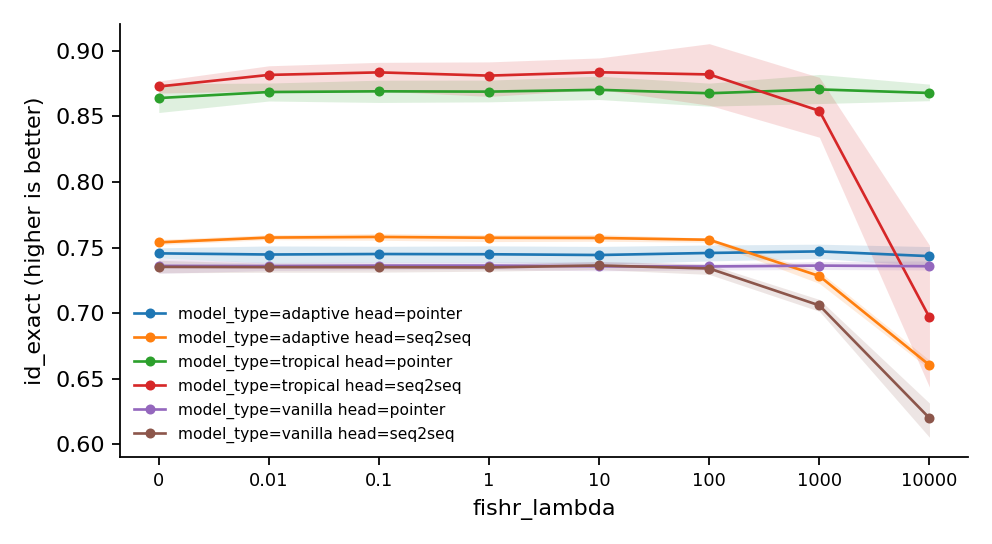
\includegraphics[width=\textwidth]{metric_id_exact.png}
\caption{\texttt{id\_exact} against \texttt{fishr\_lambda}: the mean over seeds with a 95\% bootstrap CI, one line per combination of the other factors.}
\label{fig:id_exact}
\end{figure}

{\small
\begin{longtable}{lllrlrrr}
\caption{\texttt{id\_exact} per cell: mean, 95\% bootstrap CI, SD, seeds, diverged runs.}\label{tab:summary-id_exact}\\
\toprule
\texttt{model\_type} & \texttt{head} & \texttt{fishr\_lambda} & mean & 95\% CI & SD & $n$ & div.\\
\midrule
\endhead
adaptive & pointer & 0 & 0.7455 & [0.742, 0.75] & 0.00499 & 5 & 0\\
adaptive & pointer & 0.01 & 0.7447 & [0.738, 0.751] & 0.00832 & 5 & 0\\
adaptive & pointer & 0.1 & 0.745 & [0.739, 0.751] & 0.00778 & 5 & 0\\
adaptive & pointer & 1 & 0.7449 & [0.739, 0.751] & 0.00817 & 5 & 0\\
adaptive & pointer & 10 & 0.7443 & [0.737, 0.751] & 0.00855 & 5 & 0\\
adaptive & pointer & 100 & 0.7458 & [0.74, 0.752] & 0.00822 & 5 & 0\\
adaptive & pointer & 1000 & 0.747 & [0.742, 0.753] & 0.00719 & 5 & 0\\
adaptive & pointer & 1e+04 & 0.7434 & [0.736, 0.751] & 0.00936 & 5 & 0\\
adaptive & seq2seq & 0 & 0.7539 & [0.752, 0.756] & 0.00256 & 5 & 0\\
adaptive & seq2seq & 0.01 & 0.7576 & [0.756, 0.76] & 0.00235 & 5 & 0\\
adaptive & seq2seq & 0.1 & 0.7581 & [0.756, 0.761] & 0.00329 & 5 & 0\\
adaptive & seq2seq & 1 & 0.7574 & [0.755, 0.76] & 0.00334 & 5 & 0\\
adaptive & seq2seq & 10 & 0.7573 & [0.755, 0.76] & 0.00326 & 5 & 0\\
adaptive & seq2seq & 100 & 0.7559 & [0.754, 0.757] & 0.00212 & 5 & 0\\
adaptive & seq2seq & 1000 & 0.7282 & [0.723, 0.732] & 0.00612 & 5 & 0\\
adaptive & seq2seq & 1e+04 & 0.6602 & [0.657, 0.664] & 0.00442 & 5 & 0\\
tropical & pointer & 0 & 0.8641 & [0.853, 0.875] & 0.0145 & 5 & 0\\
tropical & pointer & 0.01 & 0.8687 & [0.862, 0.876] & 0.00872 & 5 & 0\\
tropical & pointer & 0.1 & 0.8692 & [0.861, 0.878] & 0.0112 & 5 & 0\\
tropical & pointer & 1 & 0.869 & [0.861, 0.878] & 0.0108 & 5 & 0\\
tropical & pointer & 10 & 0.8704 & [0.863, 0.881] & 0.0118 & 5 & 0\\
tropical & pointer & 100 & 0.8677 & [0.858, 0.875] & 0.011 & 5 & 0\\
tropical & pointer & 1000 & 0.8707 & [0.86, 0.882] & 0.0147 & 5 & 0\\
tropical & pointer & 1e+04 & 0.868 & [0.862, 0.875] & 0.00788 & 5 & 0\\
tropical & seq2seq & 0 & 0.8729 & [0.868, 0.877] & 0.00606 & 5 & 0\\
tropical & seq2seq & 0.01 & 0.8817 & [0.87, 0.889] & 0.0137 & 5 & 0\\
tropical & seq2seq & 0.1 & 0.8837 & [0.869, 0.891] & 0.0158 & 5 & 0\\
tropical & seq2seq & 1 & 0.8812 & [0.865, 0.892] & 0.0172 & 5 & 0\\
tropical & seq2seq & 10 & 0.8838 & [0.871, 0.895] & 0.0154 & 5 & 0\\
tropical & seq2seq & 100 & 0.8821 & [0.859, 0.906] & 0.0287 & 5 & 0\\
tropical & seq2seq & 1000 & 0.8543 & [0.834, 0.88] & 0.0295 & 5 & 0\\
tropical & seq2seq & 1e+04 & 0.6967 & [0.643, 0.752] & 0.0723 & 5 & 0\\
vanilla & pointer & 0 & 0.736 & [0.73, 0.742] & 0.00749 & 5 & 0\\
vanilla & pointer & 0.01 & 0.7359 & [0.732, 0.739] & 0.00398 & 5 & 0\\
vanilla & pointer & 0.1 & 0.7362 & [0.733, 0.739] & 0.00384 & 5 & 0\\
vanilla & pointer & 1 & 0.7362 & [0.733, 0.739] & 0.00376 & 5 & 0\\
vanilla & pointer & 10 & 0.7356 & [0.732, 0.739] & 0.00463 & 5 & 0\\
vanilla & pointer & 100 & 0.7355 & [0.733, 0.738] & 0.00324 & 5 & 0\\
vanilla & pointer & 1000 & 0.7362 & [0.733, 0.739] & 0.00396 & 5 & 0\\
vanilla & pointer & 1e+04 & 0.7357 & [0.733, 0.74] & 0.00461 & 5 & 0\\
vanilla & seq2seq & 0 & 0.7352 & [0.731, 0.74] & 0.00612 & 5 & 0\\
vanilla & seq2seq & 0.01 & 0.735 & [0.731, 0.738] & 0.00458 & 5 & 0\\
vanilla & seq2seq & 0.1 & 0.735 & [0.731, 0.738] & 0.0044 & 5 & 0\\
vanilla & seq2seq & 1 & 0.7348 & [0.732, 0.737] & 0.00338 & 5 & 0\\
vanilla & seq2seq & 10 & 0.7363 & [0.733, 0.739] & 0.0042 & 5 & 0\\
vanilla & seq2seq & 100 & 0.734 & [0.729, 0.737] & 0.005 & 5 & 0\\
vanilla & seq2seq & 1000 & 0.7058 & [0.701, 0.71] & 0.00616 & 5 & 0\\
vanilla & seq2seq & 1e+04 & 0.6198 & [0.605, 0.631] & 0.0176 & 5 & 0\\
\bottomrule
\end{longtable}
}

{\small
\begin{longtable}{lllrrrl}
\caption{\texttt{id\_exact}: each level of \texttt{fishr\_lambda} against its control (0), within each combination of the other factors. parametric: Dunnett vs control.}\label{tab:control-id_exact}\\
\toprule
\texttt{model\_type} & \texttt{head} & \texttt{fishr\_lambda} & difference & 95\% CI & $p$ & \\
\midrule
\endhead
adaptive & pointer & 0.01 & $-8.800\times10^{-4}$ & [-0.0147, 0.0129] & 1.0000 & \\
adaptive & pointer & 0.1 & $-5.000\times10^{-4}$ & [-0.0143, 0.0133] & 1.0000 & \\
adaptive & pointer & 1 & $-6.800\times10^{-4}$ & [-0.0145, 0.0131] & 1.0000 & \\
adaptive & pointer & 10 & -0.00126 & [-0.0151, 0.0126] & 0.9999 & \\
adaptive & pointer & 100 & $3.000\times10^{-4}$ & [-0.0135, 0.0141] & 1.0000 & \\
adaptive & pointer & 1000 & 0.0015 & [-0.0123, 0.0153] & 0.9998 & \\
adaptive & pointer & 1e+04 & -0.00212 & [-0.0159, 0.0117] & 0.9983 & \\
adaptive & seq2seq & 0.01 & 0.00366 & [-0.0027, 0.01] & 0.4589 & \\
adaptive & seq2seq & 0.1 & 0.00414 & [-0.00222, 0.0105] & 0.3347 & \\
adaptive & seq2seq & 1 & 0.0035 & [-0.00286, 0.00986] & 0.5049 & \\
adaptive & seq2seq & 10 & 0.00334 & [-0.00302, 0.0097] & 0.5525 & \\
adaptive & seq2seq & 100 & 0.00198 & [-0.00438, 0.00834] & 0.9215 & \\
adaptive & seq2seq & 1000 & -0.02572 & [-0.0321, -0.0194] & $<10^{-4}$ & *\\
adaptive & seq2seq & 1e+04 & -0.0937 & [-0.1, -0.0873] & $<10^{-4}$ & *\\
tropical & pointer & 0.01 & 0.0046 & [-0.0156, 0.0248] & 0.9830 & \\
tropical & pointer & 0.1 & 0.00514 & [-0.0151, 0.0253] & 0.9697 & \\
tropical & pointer & 1 & 0.0049 & [-0.0153, 0.0251] & 0.9763 & \\
tropical & pointer & 10 & 0.00628 & [-0.0139, 0.0265] & 0.9219 & \\
tropical & pointer & 100 & 0.00366 & [-0.0165, 0.0239] & 0.9953 & \\
tropical & pointer & 1000 & 0.00658 & [-0.0136, 0.0268] & 0.9046 & \\
tropical & pointer & 1e+04 & 0.00388 & [-0.0163, 0.0241] & 0.9934 & \\
tropical & seq2seq & 0.01 & 0.00884 & [-0.0462, 0.0638] & 0.9977 & \\
tropical & seq2seq & 0.1 & 0.01078 & [-0.0442, 0.0658] & 0.9926 & \\
tropical & seq2seq & 1 & 0.0083 & [-0.0467, 0.0633] & 0.9985 & \\
tropical & seq2seq & 10 & 0.01086 & [-0.0441, 0.0659] & 0.9923 & \\
tropical & seq2seq & 100 & 0.0092 & [-0.0458, 0.0642] & 0.9971 & \\
tropical & seq2seq & 1000 & -0.01856 & [-0.0736, 0.0364] & 0.8896 & \\
tropical & seq2seq & 1e+04 & -0.1762 & [-0.231, -0.121] & $<10^{-4}$ & *\\
vanilla & pointer & 0.01 & $-1.000\times10^{-4}$ & [-0.00814, 0.00794] & 1.0000 & \\
vanilla & pointer & 0.1 & $2.000\times10^{-4}$ & [-0.00784, 0.00824] & 1.0000 & \\
vanilla & pointer & 1 & $2.400\times10^{-4}$ & [-0.0078, 0.00828] & 1.0000 & \\
vanilla & pointer & 10 & $-3.400\times10^{-4}$ & [-0.00838, 0.0077] & 1.0000 & \\
vanilla & pointer & 100 & $-4.600\times10^{-4}$ & [-0.0085, 0.00758] & 1.0000 & \\
vanilla & pointer & 1000 & $2.200\times10^{-4}$ & [-0.00782, 0.00826] & 1.0000 & \\
vanilla & pointer & 1e+04 & $-2.600\times10^{-4}$ & [-0.0083, 0.00778] & 1.0000 & \\
vanilla & seq2seq & 0.01 & $-2.000\times10^{-4}$ & [-0.0137, 0.0133] & 1.0000 & \\
vanilla & seq2seq & 0.1 & $-2.600\times10^{-4}$ & [-0.0138, 0.0133] & 1.0000 & \\
vanilla & seq2seq & 1 & $-4.200\times10^{-4}$ & [-0.014, 0.0131] & 1.0000 & \\
vanilla & seq2seq & 10 & 0.00108 & [-0.0125, 0.0146] & 1.0000 & \\
vanilla & seq2seq & 100 & -0.00124 & [-0.0148, 0.0123] & 0.9999 & \\
vanilla & seq2seq & 1000 & -0.0294 & [-0.0429, -0.0159] & $<10^{-4}$ & *\\
vanilla & seq2seq & 1e+04 & -0.1154 & [-0.129, -0.102] & $<10^{-4}$ & *\\
\bottomrule
\end{longtable}
}

{\small
\begin{longtable}{llrrrrr}
\caption{\texttt{id\_exact} against log10 \texttt{fishr\_lambda}: parametric: OLS slope t-test, seed-bootstrap CI, with the Jonckheere--Terpstra ordered-trend $\tau$ and $p$.}\label{tab:trend-id_exact}\\
\toprule
\texttt{model\_type} & \texttt{head} & estimate & 95\% CI & $p$ & JT $\tau$ & JT $p$\\
\midrule
\endhead
adaptive & pointer & $4.500\times10^{-5}$ & [$-2.57\times10^{-4}$, $3.19\times10^{-4}$] & 0.9451 & 0.0533 & 0.7009\\
adaptive & seq2seq & -0.01262 & [-0.0135, -0.0118] & $<10^{-4}$ & -0.608 & 0.0002\\
tropical & pointer & $-1.857\times10^{-5}$ & [$-2.36\times10^{-4}$, $1.28\times10^{-4}$] & 0.9830 & 0.0381 & 0.7780\\
tropical & seq2seq & -0.02189 & [-0.0288, -0.0144] & $<10^{-4}$ & -0.451 & 0.0004\\
vanilla & pointer & $-4.071\times10^{-5}$ & [$-4.24\times10^{-4}$, $3.46\times10^{-4}$] & 0.8977 & -0.0286 & 0.8376\\
vanilla & seq2seq & -0.01446 & [-0.0164, -0.0126] & $<10^{-4}$ & -0.543 & 0.0002\\
\bottomrule
\end{longtable}
}

{\small
\begin{longtable}{lrrrl}
\caption{\texttt{id\_exact}: paired contrasts by seed, Holm-corrected across the cells. parametric: paired t-test by seed, Holm.}\label{tab:paired-id_exact}\\
\toprule
contrast (within) & difference & 95\% CI & $p$ & \\
\midrule
\endhead
\stackcell{model\_type: tropical - vanilla\\\footnotesize head=pointer fishr\_lambda=0 } & 0.1281 & [0.105, 0.151] & 0.0004 & *\\
\stackcell{model\_type: tropical - vanilla\\\footnotesize head=pointer fishr\_lambda=0.01 } & 0.1328 & [0.121, 0.145] & $<10^{-4}$ & *\\
\stackcell{model\_type: tropical - vanilla\\\footnotesize head=pointer fishr\_lambda=0.1 } & 0.133 & [0.118, 0.148] & 0.0002 & *\\
\stackcell{model\_type: tropical - vanilla\\\footnotesize head=pointer fishr\_lambda=1 } & 0.1328 & [0.119, 0.147] & 0.0001 & *\\
\stackcell{model\_type: tropical - vanilla\\\footnotesize head=pointer fishr\_lambda=10 } & 0.1347 & [0.117, 0.152] & 0.0003 & *\\
\stackcell{model\_type: tropical - vanilla\\\footnotesize head=pointer fishr\_lambda=100 } & 0.1322 & [0.119, 0.145] & 0.0001 & *\\
\stackcell{model\_type: tropical - vanilla\\\footnotesize head=pointer fishr\_lambda=1000 } & 0.1345 & [0.115, 0.154] & 0.0004 & *\\
\stackcell{model\_type: tropical - vanilla\\\footnotesize head=pointer fishr\_lambda=1e+04 } & 0.1322 & [0.121, 0.144] & $<10^{-4}$ & *\\
\stackcell{model\_type: tropical - vanilla\\\footnotesize head=seq2seq fishr\_lambda=0 } & 0.1377 & [0.128, 0.148] & $<10^{-4}$ & *\\
\stackcell{model\_type: tropical - vanilla\\\footnotesize head=seq2seq fishr\_lambda=0.01 } & 0.1467 & [0.127, 0.167] & 0.0003 & *\\
\stackcell{model\_type: tropical - vanilla\\\footnotesize head=seq2seq fishr\_lambda=0.1 } & 0.1487 & [0.126, 0.171] & 0.0004 & *\\
\stackcell{model\_type: tropical - vanilla\\\footnotesize head=seq2seq fishr\_lambda=1 } & 0.1464 & [0.123, 0.169] & 0.0004 & *\\
\stackcell{model\_type: tropical - vanilla\\\footnotesize head=seq2seq fishr\_lambda=10 } & 0.1475 & [0.126, 0.169] & 0.0004 & *\\
\stackcell{model\_type: tropical - vanilla\\\footnotesize head=seq2seq fishr\_lambda=100 } & 0.1481 & [0.111, 0.185] & 0.0007 & *\\
\stackcell{model\_type: tropical - vanilla\\\footnotesize head=seq2seq fishr\_lambda=1000 } & 0.1485 & [0.118, 0.179] & 0.0005 & *\\
\stackcell{model\_type: tropical - vanilla\\\footnotesize head=seq2seq fishr\_lambda=1e+04 } & 0.07686 & [-0.00626, 0.16] & 0.0622 & \\
\stackcell{model\_type: adaptive - vanilla\\\footnotesize head=pointer fishr\_lambda=0 } & 0.00956 & [$5.64\times10^{-4}$, 0.0186] & 0.3356 & \\
\stackcell{model\_type: adaptive - vanilla\\\footnotesize head=pointer fishr\_lambda=0.01 } & 0.00878 & [-0.00352, 0.0211] & 0.4752 & \\
\stackcell{model\_type: adaptive - vanilla\\\footnotesize head=pointer fishr\_lambda=0.1 } & 0.00886 & [-0.00244, 0.0202] & 0.4752 & \\
\stackcell{model\_type: adaptive - vanilla\\\footnotesize head=pointer fishr\_lambda=1 } & 0.00864 & [-0.00363, 0.0209] & 0.4752 & \\
\stackcell{model\_type: adaptive - vanilla\\\footnotesize head=pointer fishr\_lambda=10 } & 0.00864 & [-0.0042, 0.0215] & 0.4752 & \\
\stackcell{model\_type: adaptive - vanilla\\\footnotesize head=pointer fishr\_lambda=100 } & 0.01032 & [-0.00154, 0.0222] & 0.4383 & \\
\stackcell{model\_type: adaptive - vanilla\\\footnotesize head=pointer fishr\_lambda=1000 } & 0.01084 & [$1.54\times10^{-4}$, 0.0215] & 0.3360 & \\
\stackcell{model\_type: adaptive - vanilla\\\footnotesize head=pointer fishr\_lambda=1e+04 } & 0.0077 & [-0.0061, 0.0215] & 0.4752 & \\
\stackcell{model\_type: adaptive - vanilla\\\footnotesize head=seq2seq fishr\_lambda=0 } & 0.01872 & [0.00993, 0.0275] & 0.0410 & *\\
\stackcell{model\_type: adaptive - vanilla\\\footnotesize head=seq2seq fishr\_lambda=0.01 } & 0.02258 & [0.018, 0.0272] & 0.0022 & *\\
\stackcell{model\_type: adaptive - vanilla\\\footnotesize head=seq2seq fishr\_lambda=0.1 } & 0.02312 & [0.0198, 0.0264] & 0.0006 & *\\
\stackcell{model\_type: adaptive - vanilla\\\footnotesize head=seq2seq fishr\_lambda=1 } & 0.02264 & [0.0184, 0.0269] & 0.0017 & *\\
\stackcell{model\_type: adaptive - vanilla\\\footnotesize head=seq2seq fishr\_lambda=10 } & 0.02098 & [0.0187, 0.0233] & 0.0002 & *\\
\stackcell{model\_type: adaptive - vanilla\\\footnotesize head=seq2seq fishr\_lambda=100 } & 0.02194 & [0.0156, 0.0283] & 0.0074 & *\\
\stackcell{model\_type: adaptive - vanilla\\\footnotesize head=seq2seq fishr\_lambda=1000 } & 0.0224 & [0.0172, 0.0276] & 0.0034 & *\\
\stackcell{model\_type: adaptive - vanilla\\\footnotesize head=seq2seq fishr\_lambda=1e+04 } & 0.04044 & [0.021, 0.0599] & 0.0410 & *\\
\stackcell{head: pointer - seq2seq\\\footnotesize model\_type=adaptive fishr\_lambda=0 } & -0.0084 & [-0.0119, -0.00495] & 0.0526 & \\
\stackcell{head: pointer - seq2seq\\\footnotesize model\_type=adaptive fishr\_lambda=0.01 } & -0.01294 & [-0.0239, -0.00202] & 0.5130 & \\
\stackcell{head: pointer - seq2seq\\\footnotesize model\_type=adaptive fishr\_lambda=0.1 } & -0.01304 & [-0.0247, -0.00136] & 0.5802 & \\
\stackcell{head: pointer - seq2seq\\\footnotesize model\_type=adaptive fishr\_lambda=1 } & -0.01258 & [-0.0253, $1.67\times10^{-4}$] & 0.7786 & \\
\stackcell{head: pointer - seq2seq\\\footnotesize model\_type=adaptive fishr\_lambda=10 } & -0.013 & [-0.0231, -0.00287] & 0.4228 & \\
\stackcell{head: pointer - seq2seq\\\footnotesize model\_type=adaptive fishr\_lambda=100 } & -0.01008 & [-0.0215, 0.00137] & 0.9933 & \\
\stackcell{head: pointer - seq2seq\\\footnotesize model\_type=adaptive fishr\_lambda=1000 } & 0.01882 & [0.0047, 0.0329] & 0.3955 & \\
\stackcell{head: pointer - seq2seq\\\footnotesize model\_type=adaptive fishr\_lambda=1e+04 } & 0.08318 & [0.0668, 0.0996] & 0.0033 & *\\
\stackcell{head: pointer - seq2seq\\\footnotesize model\_type=tropical fishr\_lambda=0 } & -0.00882 & [-0.0229, 0.0053] & 1.0000 & \\
\stackcell{head: pointer - seq2seq\\\footnotesize model\_type=tropical fishr\_lambda=0.01 } & -0.01306 & [-0.0288, 0.00266] & 1.0000 & \\
\stackcell{head: pointer - seq2seq\\\footnotesize model\_type=tropical fishr\_lambda=0.1 } & -0.01446 & [-0.0334, 0.0045] & 1.0000 & \\
\stackcell{head: pointer - seq2seq\\\footnotesize model\_type=tropical fishr\_lambda=1 } & -0.01222 & [-0.0331, 0.00861] & 1.0000 & \\
\stackcell{head: pointer - seq2seq\\\footnotesize model\_type=tropical fishr\_lambda=10 } & -0.0134 & [-0.0345, 0.00773] & 1.0000 & \\
\stackcell{head: pointer - seq2seq\\\footnotesize model\_type=tropical fishr\_lambda=100 } & -0.01436 & [-0.0473, 0.0186] & 1.0000 & \\
\stackcell{head: pointer - seq2seq\\\footnotesize model\_type=tropical fishr\_lambda=1000 } & 0.01632 & [-0.0238, 0.0564] & 1.0000 & \\
\stackcell{head: pointer - seq2seq\\\footnotesize model\_type=tropical fishr\_lambda=1e+04 } & 0.1713 & [0.0775, 0.265] & 0.1428 & \\
\stackcell{head: pointer - seq2seq\\\footnotesize model\_type=vanilla fishr\_lambda=0 } & $7.600\times10^{-4}$ & [-0.0148, 0.0163] & 1.0000 & \\
\stackcell{head: pointer - seq2seq\\\footnotesize model\_type=vanilla fishr\_lambda=0.01 } & $8.600\times10^{-4}$ & [-0.00886, 0.0106] & 1.0000 & \\
\stackcell{head: pointer - seq2seq\\\footnotesize model\_type=vanilla fishr\_lambda=0.1 } & 0.00122 & [-0.00809, 0.0105] & 1.0000 & \\
\stackcell{head: pointer - seq2seq\\\footnotesize model\_type=vanilla fishr\_lambda=1 } & 0.00142 & [-0.00566, 0.0085] & 1.0000 & \\
\stackcell{head: pointer - seq2seq\\\footnotesize model\_type=vanilla fishr\_lambda=10 } & $-6.600\times10^{-4}$ & [-0.00988, 0.00856] & 1.0000 & \\
\stackcell{head: pointer - seq2seq\\\footnotesize model\_type=vanilla fishr\_lambda=100 } & 0.00154 & [-0.00683, 0.00991] & 1.0000 & \\
\stackcell{head: pointer - seq2seq\\\footnotesize model\_type=vanilla fishr\_lambda=1000 } & 0.03038 & [0.026, 0.0348] & 0.0011 & *\\
\stackcell{head: pointer - seq2seq\\\footnotesize model\_type=vanilla fishr\_lambda=1e+04 } & 0.1159 & [0.0976, 0.134] & 0.0014 & *\\
\bottomrule
\end{longtable}
}


\section{Curves}
\begin{figure}[tbp]
\centering
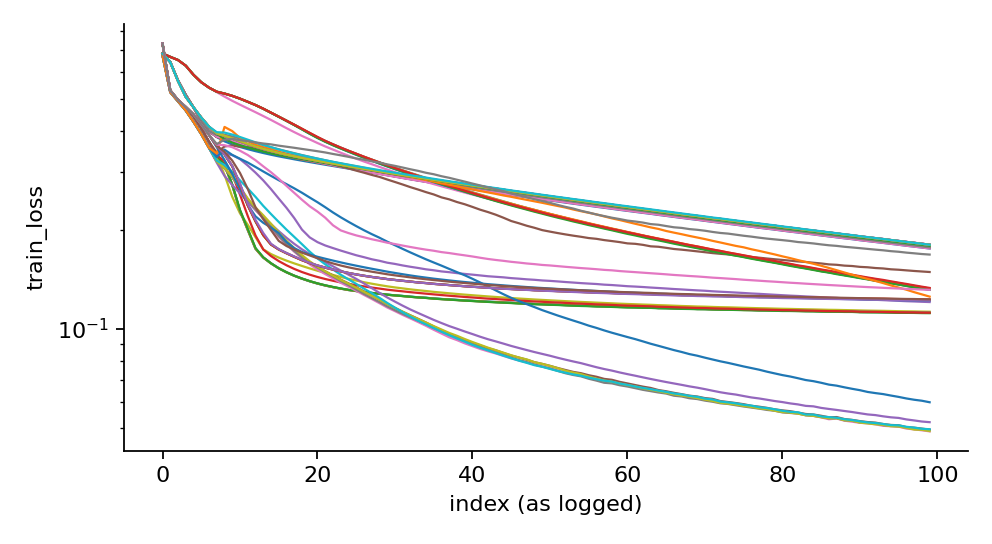
\includegraphics[width=\textwidth]{curve_train_loss.png}
\caption{\texttt{train\_loss}, the mean over seeds per cell.}
\label{fig:curve-1}
\end{figure}
\begin{figure}[tbp]
\centering
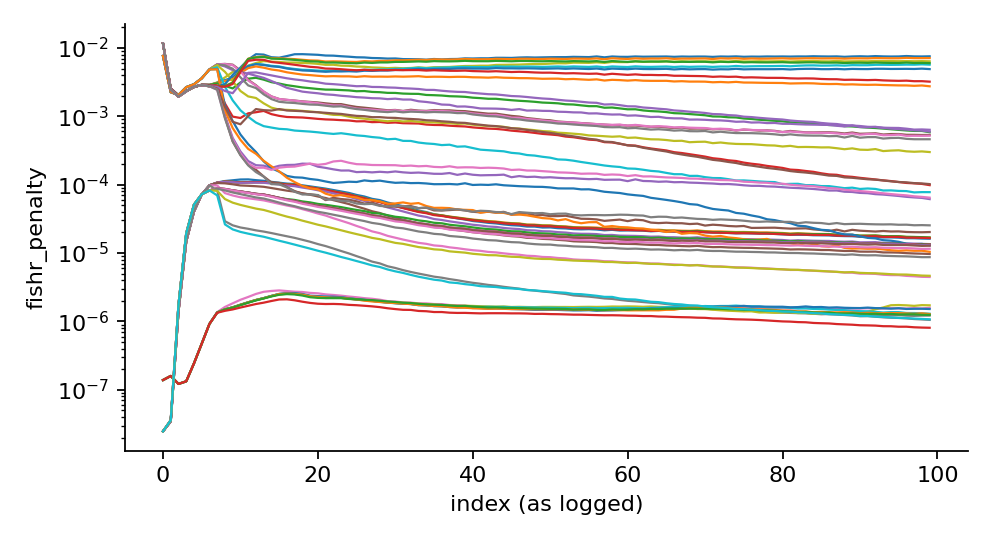
\includegraphics[width=\textwidth]{curve_fishr_penalty.png}
\caption{\texttt{fishr\_penalty}, the mean over seeds per cell.}
\label{fig:curve-2}
\end{figure}
\begin{figure}[tbp]
\centering
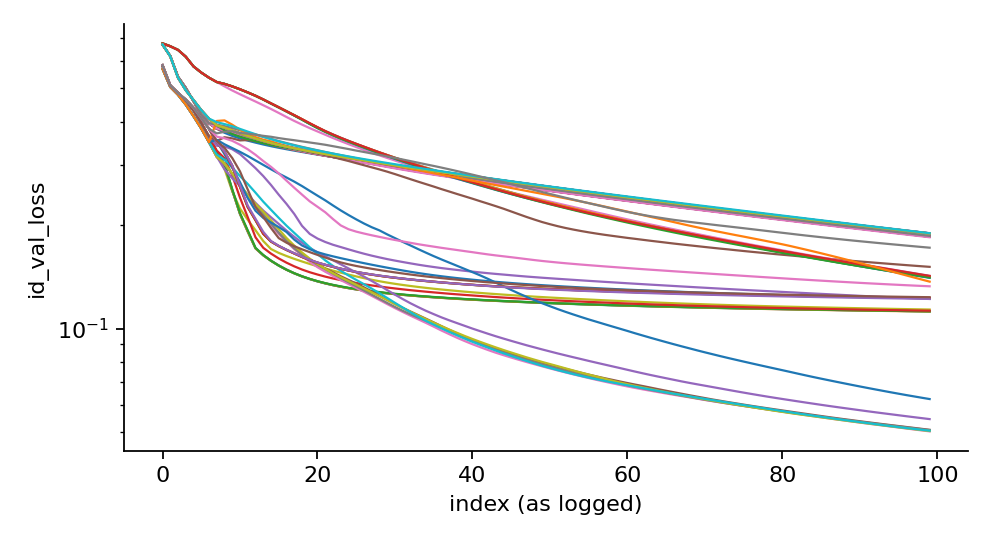
\includegraphics[width=\textwidth]{curve_id_val_loss.png}
\caption{\texttt{id\_val\_loss}, the mean over seeds per cell.}
\label{fig:curve-3}
\end{figure}

\section{Configuration}
The base configuration every run shares (frozen hash \texttt{aff15420a136}); factor levels are in \autoref{tab:summary-ood_len_f1}.
{\footnotesize
\begin{verbatim}
task:
  name: ConvexHullDataset
  value_range:
  - 0
  - 10
  target_range: null
  weight_range: null
  adversarial_range:
  - 10
  - 30
  noise_prob: 0.0
data:
  train_lengths:
  - 4
  - 5
  - 6
  - 7
  - 8
  ood_lengths:
  - 12
  - 16
  - 64
  ood_value_range:
  - 11
  - 21
  ood_noise_range:
  - 1
  - 5
  ood_noise_prob: 0.5
  n_per_length: 20000
  n_eval_per_length: 2000
  curve_eval_limit: 256
model:
  d_model: 64
  n_heads: 2
  num_layers: 1
  dropout: 0.0
  tropical_impl: legacy
optim:
  lr: 0.0001
  epochs: 100
  batch_size: 100
  eval_batch_size: 256
fishr:
  ema: 0.95
  anneal_iters: 1500
  reset_optimizer: true
\end{verbatim}
}
Store: \texttt{campaigns/tropical/ConvexHull/results}.
\end{document}